% !TEX root = base.tex

% !TEX root = ./base.tex
%% abtex2-modelo-trabalho-academico.tex, v-1.9.5 laurocesar
%% Copyright 2012-2015 by abnTeX2 group at http://www.abntex.net.br/ 
%%
%% This work may be distributed and/or modified under the
%% conditions of the LaTeX Project Public License, either version 1.3
%% of this license or (at your option) any later version.
%% The latest version of this license is in
%%   http://www.latex-project.org/lppl.txt
%% and version 1.3 or later is part of all distributions of LaTeX
%% version 2005/12/01 or later.
%%
%% This work has the LPPL maintenance status `maintained'.
%% 
%% The Current Maintainer of this work is the abnTeX2 team, led
%% by Lauro César Araujo. Further information are available on 
%% http://www.abntex.net.br/
%%
%% This work consists of the files abntex2-modelo-trabalho-academico.tex,
%% abntex2-modelo-include-comandos and abntex2-modelo-references.bib
%%

% ------------------------------------------------------------------------
% ------------------------------------------------------------------------
% abnTeX2: Modelo de Trabalho Academico (tese de doutorado, dissertacao de
% mestrado e trabalhos monograficos em geral) em conformidade com 
% ABNT NBR 14724:2011: Informacao e documentacao - Trabalhos academicos -
% Apresentacao
% ------------------------------------------------------------------------
% ------------------------------------------------------------------------

\documentclass[
  % -- opções da classe memoir --
  12pt,        % tamanho da fonte
  openright,      % capítulos começam em pág ímpar (insere página vazia caso preciso)
  oneside,      % para impressão apenas no verso. Oposto a twoside
  % twoside,      % para impressão em verso e anverso. Oposto a oneside
  a4paper,      % tamanho do papel. 
  % -- opções da classe abntex2 --
  %chapter=TITLE,    % títulos de capítulos convertidos em letras maiúsculas
  %section=TITLE,    % títulos de seções convertidos em letras maiúsculas
  %subsection=TITLE,  % títulos de subseções convertidos em letras maiúsculas
  %subsubsection=TITLE,% títulos de subsubseções convertidos em letras maiúsculas
  % -- opções do pacote babel --
  english,      % idioma adicional para hifenização
  french,        % idioma adicional para hifenização
  spanish,      % idioma adicional para hifenização
  brazil        % o último idioma é o principal do documento
]{abntex2}

% ---
% Pacotes básicos 
% ---
\usepackage{lmodern}      % Usa a fonte Latin Modern      
\usepackage[T1]{fontenc}    % Selecao de codigos de fonte.
\usepackage[utf8]{inputenc}    % Codificacao do documento (conversão automática dos acentos)
\usepackage{lastpage}      % Usado pela Ficha catalográfica
\usepackage{indentfirst}    % Indenta o primeiro parágrafo de cada seção.
\usepackage{color}        % Controle das cores
\usepackage{graphicx}      % Inclusão de gráficos
\usepackage{microtype}       % para melhorias de justificação
\usepackage{booktabs}
\usepackage{graphicx}
\usepackage[table,xcdraw]{xcolor}
\usepackage{float}
% ---

% ---
% Pacotes adicionais, usados apenas no âmbito do Modelo Canônico do abnteX2
% ---
\usepackage{lipsum}        % para geração de dummy text
% ---

% --- Pacotes de citações ---

\usepackage[brazilian,hyperpageref]{backref}   % Paginas com as citações na bibl
\usepackage[alf]{abntex2cite}  % Citações padrão ABNT

% --- 
% CONFIGURAÇÕES DE PACOTES
% --- 

% ---
% Configurações do pacote backref
% Usado sem a opção hyperpageref de backref
\renewcommand{\backrefpagesname}{Citado na(s) página(s):~} % Texto padrão antes do número das páginas

\renewcommand{\backref}{}
% Define os textos da citação
\renewcommand*{\backrefalt}[4]{
  \ifcase#1 %
    Nenhuma citação no texto.%
  \or{}
    Citado na página #2.%
  \else
    Citado #1 vezes nas páginas #2.%
  \fi}%
% ---
\setlength{\parindent}{1.3cm} % --- Espaçamentos entre linhas e parágrafos --- % 
\setlength{\parskip}{0.2cm}  % Controle do espaçamento entre um parágrafo e outro: tente também \onelineskip
% Seleciona o idioma do documento (conforme pacotes do babel)
%\selectlanguage{english}
\selectlanguage{brazil}
\frenchspacing % Retira espaço extra obsoleto entre as frases.
\makeindex % --- compila o indice --- %


% ADIÇÕES FEITAS POR MIM (João Vítor Fernandes Dias)

% \usepackage{fontspec} % Adicionar emoji
% \usepackage{parskip} % Adicionar emoji?
\usepackage{booktabs} % Necessários pra tabela
\usepackage{multirow} % Necessários pra tabela
\usepackage{listings} % Necessário para código

% Necessário para códigos bonitos

\definecolor{codegreen}{HTML}{009900}
\definecolor{codegray}{HTML}{808080}
\definecolor{codepurple}{HTML}{9400D3}
\definecolor{backcolour}{HTML}{F2F2EB}

\lstdefinestyle{mystyle}{
  backgroundcolor=\color{backcolour},
  commentstyle=\color{codegreen},
  keywordstyle=\color{magenta},
  numberstyle=\tiny\color{codegray},
  stringstyle=\color{codepurple},
  basicstyle=\ttfamily\footnotesize,
  breakatwhitespace=false,
  breaklines=true,
  captionpos=b,
  keepspaces=true,
  numbers=left,
  numbersep=5pt,
  showspaces=false,
  showstringspaces=false,
  showtabs=false,
  tabsize=2
}

\lstset{style=mystyle}

\renewcommand{\lstlistingname}{Código}% Listing -> Código
\renewcommand{\lstlistlistingname}{Lista de \lstlistingname s} % List of Listings -> Lista de Códigos

\usepackage{tikz}
\usepackage{animate}

% --- Informações de dados para CAPA e FOLHA DE ROSTO --- %

\autor{João Vítor Fernandes Dias}
\titulo{\textit{Timetabling Problem}: desafios no desenvolvimento de um sistema de decisão voltado ao problema de organização de grade horária do ensino superior}
\local{Campos dos Goytacazes, RJ}
\data{\today}

\def\orientadorTCC{FermÍn Alfredo Tang Montané}

\preambulo{Trabalho de Conclusão de Curso apresentado ao Curso de Graduação em Ciência da Computação da Universidade Estadual do Norte Fluminense Darcy Ribeiro, sob orientação do Prof. Dr. \orientadorTCC}
% \instituicao{Universidade Estadual do Norte Fluminense Darcy Ribeiro \par Ciência da Computação \par Metodologia de Pesquisa}
\orientador{\orientadorTCC}
\tipotrabalho{Projeto de Pesquisa}
%\coorientador{Equipe \abnTeX}
% O preambulo deve conter o tipo do trabalho, o objetivo, o nome da instituição e a área de concentração
% ---

% ---
% Configurações de aparência do PDF final
% alterando o aspecto da cor azul
\definecolor{blue}{RGB}{41,5,195}

% informações do PDF
\makeatletter
\hypersetup{
%pagebackref=true,
    pdftitle={\@title}, 
    pdfauthor={\@author},
    pdfsubject={\imprimirpreambulo},
    pdfcreator={LaTeX with abnTeX2},
    pdfkeywords={abnt}{latex}{abntex}{abntex2}{trabalho acadêmico}, 
    colorlinks=true,       		% false: boxed links; true: colored links
    linkcolor=blue,          	% color of internal links
    citecolor=blue,        		% color of links to bibliography
    filecolor=magenta,      		% color of file links
    urlcolor=blue,
    bookmarksdepth=4
}
\makeatother

\begin{document} % --- Início do documento ---
\pretextual{} % --- INÍCIO DOS ELEMENTOS PRÉ-TEXTUAIS ---

% \imprimircapa{} % Capa
% \imprimirfolhaderosto{} % Folha de rosto (o * indica que haverá a ficha bibliográfica)

% \chapter*{Banca}
% \begin{agradecimentos}
Agradeço aos meus pais que se dedicaram para que eu pudesse estar cursando esta graduação, assim podendo completar mais uma etapa da minha vida. 
Sem o apoio, conselhos, carinho e amor, nada disso seria possível. Sou eternamente grato por tudo que vocês fazem e sempre fizeram para que minha vida fosse especial. 

Agradeço ao professor Dr. Manuel Antonio Molina Palma pela dedicação e paciência durante o lecionamento desta disciplina, e obrigado pela ajuda e por estar disponível nos momentos de necessidade.   

Por último, mas não menos importante, agradeço a toda minha família e amigos que estiveram comigo em todos os momentos da minha vida.
\end{agradecimentos}
% % resumo em português
\setlength{\absparsep}{18pt} % ajusta o espaçamento dos parágrafos do resumo
\begin{resumo}

    Este artigo visa apresentar uma análise da situação em que atualmente se encontra a criação de grades horárias na Universidade Estadual do Norte Fluminense, bem como apontar seus maiores problemas e desenvolver um sistema de decisão capaz de auxiliar diversos centros e laboratórios no desenvolvimento de suas grades horárias, buscando a otimização do uso de salas e redução dos conflitos existentes entre demandas de diferentes alunos por matérias.
    
    \textbf{Palavras-chave}: Tabela de horários, Agendamento de aulas universitárias, Heurísticas, Programação Inteira, Representação do Conhecimento, Interação Homem Computador.

\end{resumo}

% \begin{epigrafe}
  \vspace*{\fill}
  \begin{flushright}
    \textit{``Quando você não sabe alguma coisa,\\
      procura quem sabe e pergunta\\
      pra não fazer feio, nem passar vergonha.\\
      Vovô Nando, 01/12/2023}
  \end{flushright}
\end{epigrafe}
% % resumo em inglês
\begin{resumo}[Abstract]
  \begin{otherlanguage*}{english}

    This paper aims to present an analysis of the current situation of the schedule creation at the Universidade Estadual do Norte Fluminense, as well as to point out its major problems and to develop a decision system capable of helping several centers and laboratories in the development of their schedules, seeking to optimize the use of rooms and to reduce the conflicts between different students' demands for subjects.

    \vspace{\onelineskip}

    % \noindent
    \textbf{Keywords}: Timetabling, University class scheduling, Heuristics, Integer Programming, Knowledge Representation, Human Computer Interaction.

  \end{otherlanguage*}
\end{resumo}
% \pdfbookmark[0]{\contentsname}{toc}
\tableofcontents*
\cleardoublepage
% \pdfbookmark[0]{\listfigurename}{lof}
\listoffigures*
\cleardoublepage{}
% \pdfbookmark[0]{\listtablename}{lot}
\listoftables*
\cleardoublepage{}
% \pdfbookmark[0]{\lstlistlistingname}{lot}
\lstlistoflistings*
\cleardoublepage{}

\textual{} % --- INÍCIO DOS ELEMENTOS TEXTUAIS ---

% \chapter{Introdução} % ## 1. Introdução

% <!-- Fazer algumas sutis alterações no português --> 
% <!-- Fazer referência ao TCC do Ricardo falando sobre ``Já existem no mercado algumas ferramentas que prometem a geração automatizada de grades de horários'' -->
% <!-- Adicionar o que Sanya, Ricardo e Vieira 2011 falam em relação às ferramentas, buscando também um novo autor mais recente que diga o mesmo -->


% <!--    Coisas a dizer
% - A realidade do ensino superior brasileiro
%   - Muitas reprovações
%   - Grade horária confusa
%   - Professores limitados
%   - Preferências diversas     X
%     - Professores             X
%       - Horários              X
%     - Alunos
%       - Estágio               X
%       - Trabalho
%       - Formar rápido
%   - Demanda variada
%   - Caso específico da UENF   X
% -->

No ensino superior brasileiro, cada curso de uma instituição de ensino tem em seu projeto pedagógico, ou seja, no documento que rege quais as atribuições e justificativas de existência do curso, uma listagem de disciplinas a serem ministradas em cada semestre ao longo de sua duração esperada. Disciplinas estas que para serem cursadas os discentes precisam cumprir determinados requisitos. Por exemplo, é esperado que o discente apenas curse a disciplina Cálculo 2 após haver obtido a aprovação prévia na disciplina Cálculo 1.

% <!-- Perguntas
% - Pesquisar quais são as regras que todos os cursos superiores devem seguir para serem reconhecidos pelo MEC
% - Qual a definição de projeto pedagógico?
% - Todos os PPCs dos cursos apresentam a listagem das disciplinas?
% -->

Embora haja este planejamento de duração do curso, diversos fatores podem influenciar esta previsão, dentre eles podemos citar eventos como:

\begin{itemize}
  \item \textbf{Quebra de pré-requisitos}: onde o discente solicita permissão para inscrição em uma disciplina cujos pré-requisitos não são completamente cumpridos por si;
  \item \textbf{Trancamento de matrícula}: onde o discente suspende temporariamente seus estudos na instituição;
  \item \textbf{Transferência interna}: onde o discente migra entre cursos dentro da mesma instituição;
  \item \textbf{Transferência externa}: onde o discente migra entre cursos entre diferentes instituições;
  \item \textbf{Reprovações}: onde o discente não cumpre com o mínimo desempenho esperado na disciplina, geralmente está associado a ausência nas aulas e/ou desempenho inferior ao mínimo esperado nas avaliações;
  \item \textbf{Disponibilidade de professores}: onde os docentes não são suficientes para ministrar todas as disciplinas demandadas pelos discentes em um mesmo semestre.
\end{itemize}

% - Quebra de pré-requisitos: onde o discente solicita permissão para inscrição em uma disciplina cujos pré-requisitos não são completamente cumpridos por si;
% - Trancamento de matrícula: onde o discente suspende temporariamente seus estudos na instituição;
% - Transferência interna: onde o discente migra entre cursos dentro da mesma instituição;
% - Transferência externa: onde o discente migra entre cursos entre diferentes instituições;
% - Reprovações: onde o discente não cumpre com o mínimo desempenho esperado na disciplina, geralmente está associado a ausência nas aulas e/ou desempenho inferior ao mínimo esperado nas avaliações;
% - Disponibilidade de professores: onde os docentes não são suficientes para ministrar todas as disciplinas demandadas pelos discentes em um mesmo semestre.

Estes eventos tendem a, no geral, aumentar o tempo médio para conclusão do curso. Situação em sua maioria indesejada tanto pelos alunos, que mesmo durante seu estudo já visam o mercado de trabalho, quanto pelos professores e a instituição, visto que a evasão do ensino superior brasileiro é um problema existente e estudado a fim de ser minimizado.

% <!--
% - Pesquisar sobre motivos de evasão do ensino superior
% - Adicionar citação
% -->

Com isso, é esperado que a instituição busque alternativas para tornar mais dinâmica e atrativa a experiência dos discentes durante sua jornada. Uma dessas formas é tentando minimizar o impacto que as reprovações nas disciplinas causam nos semestres consecutivos. Para isso sendo então necessária uma análise das disciplinas que devem ser ministradas no próximo semestre, sendo então necessário definir \textbf{quais}, \textbf{quando}, \textbf{onde}, \textbf{por quem} e \textbf{para quem} serão ministradas. Esta tarefa, entretanto, não é trivial.

\section{Problemáticas} % ### 1.1. Problemáticas

Embora seja um problema atualmente, isso não significa que seja recente. Desde 1978 \cite{barham_simple_1978} o termo \textit{timetabling} encontra-se no meio acadêmico como o termo referente ao tabelamento de grade horária, sendo assim, é este o termo que será principalmente utilizado neste trabalho. Neste artigo de 1978 já se propunha uma forma para que se obtivesse um tabelamento otimizado, e demonstrava que o método utilizado gerava bons resultados.

Outra característica é informada por Joshua \cite{thomas_visualization_2009} que fala sobre a multidimensional do problema de timetabling. Por causa dessa questão há uma complexidade elevada para conseguir conceber visual e mentalmente de que forma os dados relacionados ao problema se estruturam, assim dificultando a elaboração de sistemas computacionais que auxiliem nessa tarefa.

Também segundo J. Miranda, embora o problema de atribuição de salas não seja novo e tenha extensa literatura a seu respeito, são poucos os que de fato implementaram um sistema para suporte de decisões. Isso se dá por diversos fatores, também listado pelo autor fazendo referência a trabalhos anteriores, sendo alguns deles a resistência organizacional a mudanças e adoção de novas tecnologias, nível de dificuldade do problema, dentre outros.

% <!--  Pegar a referência original? -->

Algumas outras características que se apresentam como problemas são a falta de otimalidade das grades horárias desenvolvidas em boa parte das instituições de ensino superior e a quantidade de tempo necessária para a criação dessas grades não-ótimas.

Considerando que situações como a descrita acima são passíveis de ocorrer, e que a tarefa de criação de grades horárias é recorrente, um sistema de suporte à decisão que supra às necessidades dos seus usuários se faz necessário.

\section{Hipótese} % ### 1.2. Hipótese

Dada as características intrínsecas ao problema de agendamento de grade horária, é esperado que os softwares atualmente existentes que lidam com este problema não apresentem completas capacidades de se moldar ao caso de uma instituição específica.

E, caso a primeira hipótese se apresente correta, o software a ser desenvolvido, assim como seus similares, se apresentará como uma solução plausível para a resolução do problema proposto embora ainda apresente melhorias possíveis a serem implementadas. O software se apresentará de tal forma que os \textit{stakeholders} que, esperadamente, decidirem não o utilizar não causarão a impossibilidade do uso do sistema.

% <!--
%- Os softwares existentes não são adequados para o caso específico
%- Embora seja possível implementar
%  - Será trabalhoso
%  - Precisará atender muitos requisitos
%  - Nem todos stakeholders aceitarão facilmente a mudança
%  - O sistema não será tão intuitivo quanto poderia ser
%  - Muitos não veem essa questão como um problema
%  - Alguns não acham necessário haver mudança no método de elaboração das grades
% -->

\section{Objetivos} % ### 1.3. Objetivos

Os objetivos deste documento podem ser divididos entre gerais e específicos, não havendo relação de superioridade de um em relação ao outro, visto que ambos igualmente nortearão o desenvolvimento da pesquisa.

\subsection{Gerais} % #### 1.3.1. Gerais

% <!--
%- Sistema de suporte à decisão
%  - Eficiente
%  - Eficaz
%  - Efetivo
%- Criar grades horárias melhores, preferencialmente ótimas
%- Reduzir tempo necessário para criação das tabelas
%- Reduzir conflitos
%- Aumentar satisfação geral com as disciplinas e horários ofertados
% -->

Como objetivos gerais, espera-se conseguir desenvolver um sistema de suporte à decisão tal que aumente a eficiência, eficácia e efetividade do processo de criação de grades horárias que semestralmente demandam extensa quantidade de tempo dos coordenadores de curso na UENF e não alcançam a otimalidade. Nesse processo, também é esperado que as grades horárias finais tragam benefícios aos alunos como forma de mais disciplinas à sua disposição. Visto que estes muitas vezes lidam com grades horárias que não contemplam suas reais demandas. Dessa forma aumentando a satisfação de todos os participantes do processo, desde os coordenadores de curso até os alunos.

\subsection{Específicos} % #### 1.3.2. Específicos

Como objetivos mais específicos, podemos listar os seguintes:

\begin{itemize}
  \item Entender de que forma os setores administrativos da UENF atualmente lidam com a questão do \textit{timetabling};
  \item Obter as demandas de aprimoramentos desejadas pelos diferentes centros e laboratórios;
  \item Modelar o sistema de resolução de \textit{timetabling} de acordo com os requisitos demandados;
  \item Encontrar o que é necessário para a adoção da aplicação de tabelamento de horário;
  \item Incentivar o uso de uma ferramenta centralizada para a otimização do \textit{Timetabling Problem}.
\end{itemize}

% - Entender de que forma os setores administrativos da UENF atualmente lidam com a questão do \textit{timetabling};
% - Obter as demandas de aprimoramentos desejadas pelos diferentes centros e laboratórios;
% - Modelar o sistema de resolução de \textit{timetabling} de acordo com os requisitos demandados;
% - Encontrar o que é necessário para a adoção da aplicação de tabelamento de horário;
% - Incentivar o uso de uma ferramenta centralizada para a otimização do \textit{Timetabling Problem}.

\section{Justificativas} % ### 1.4. Justificativas

Levando em conta a problemática evidenciada e os sucessos prévios dos artigos anteriores, vê-se grande potencial de auxílio e aumento na satisfação de todos os que utilizarem os métodos propostos. Não havendo um sistema geral que solucione todos os casos como evidenciado pelos pesquisadores da área, resta aos interessados rumarem em busca de uma solução entalhada nos moldes de sua instituição específica. Considerando que é um problema existente atualmente e que uma solução está disponível, o que se torna necessário é realizar o esforço inicial suficiente para que ocorra a quebra da inércia em que se encontram os processos ineficientes usuais para assim alcançar um melhor. Sendo assim, faz-se válida a pesquisa e desenvolvimento de um software que vise este propósito.

% <!--
% - Levando em conta a problemática e o os sucessos prévios de artigos anteriores
% - As instituições públicas idealmente deveriam ter um sistema próprio para a resolução de seus próprios conflitos
% - Não havendo o interesse ou conhecimento geral para este fim, resta aos alunos e pesquisadores interessados buscarem uma solução entalhada nos moldes de sua instituição
% - Considerando que é um problema existente na instituição e que é resolvível, sendo necessário o esforço inicial de quebrar a inércia dos processos usuais para se alcançar um melhor, faz-se válida a pesquisa e desenvolvimento de um software que vise este propósito.
% -->

\section{Metodologia} % ### 1.5. Metodologia 

% <!-- Alterar a parte final da metodologia -->

% <!--
% - Entrevistas qualitativas com stakeholders     x
%   - Adicionar perguntas aqui                    .
% - Formulário quantitativo com alunos            x
%   - Adicionar perguntas aqui                    .
% - Elicitação de requisitos                      x
%   - Falar sobre o SWEBOK                        x
% - Desenvolvimento do software                   .
%   - CI/CD                                       .
%     - Testes                                    .
%     - GitHub                                    .
%   - Programação modular                         SWEBOK
%   - Obtenção de demanda                         .
%     - Extratos                                  .
%       - Processamento e limpeza                 .
%       - Estruturando dados                      .
%     - Acadêmico                                 .
%     - Formulário                                .
%   - Criando solução inicial                     .
%   - Otimizando                                  .
%     - Algoritmos                                .
%     - Interatividade                            .
%       - Visualização                            .
% -->

Considerando as dificuldades encontradas em trabalhos anteriores, entende-se que o maior desafio será superar as especificidades que serão encontradas durante a modelagem da universidade em questão. Para isso, será inicialmente necessária uma pesquisa bibliográfica com foco no estudo das abordagens qualitativas realizadas anteriormente que obtiveram sucesso em elicitar os requisitos adequados para as instituições de ensino.

% <!--
% Adicionar referência sobre pesquisa qualitativa?
% -->

Com este conhecimento, um material inicial para a pesquisa exploratória e qualitativa deve ser desenvolvido levando em conta as questões próprias da universidade em questão, visando também coletar dados relevantes para uma futura pesquisa com maior enfoque em características emergentes que a pesquisa anterior pode levantar, similar a como foi proposto e realizado por \cite{andre_interaction_2018}.

Nesta pesquisa exploratória em formato de entrevista, algumas informações esperadas revolvem em torno das percepções dos \textit{stakeholders} do sistema proposto, sendo esses principalmente os professores, coordenadores de cursos, chefes de laboratório e diretores de centro. Estas percepções incluem o entendimento deles quanto ao método atual e às alternativas existentes, nível de insatisfação com o método atual, nível de desejo quanto à um novo método. Além disso, espera-se aproveitar o ensejo para elicitar as características e funcionalidades que gostariam de ter em um sistema de suporte à decisão, solicitando também que deem informações adicionais que gostariam de acrescentar.

Essas informações serão relevantes para se atingir a satisfação e uso futuro do sistema proposto. Pois, como é informado no \cite{bourque_swebok_2014}, uma das fontes de requisitos é o ambiente organizacional e como o software muitas vezes visa auxiliar em algum processo da instituição, processo este já condicionado à sua estrutura, cultura e políticas externas, o engenheiro de software precisa estar atento a elas, visto que o novo software não deve forçar mudanças não planejadas em processos de negócios.

Questionamentos similares também serão realizados com alunos, porém em formato de formulário online para facilitar o processamento dos dados coletados.

% <!--
\def\LinkParadigm{https://www.visual-paradigm.com/}
\def\LinkDrawio{https://www.drawio.com/}
\def\LinkMermaid{https://mermaid.js.org/}
% -->

% [LinkDrawio]: https://www.drawio.com/
% [LinkMermaid]: https://mermaid.js.org/
% [LinkVisualParadigm]: https://www.visual-paradigm.com/

Tendo obtido as informações dos \textit{stakeholders} primários, será então necessário modelar quais são as regras que ditam a estrutura organizacional em foco. Para este fim, serão utilizados diagramas conceituais utilizando softwares de suporte como o \href{https://draw.io/}{draw.io} e o \href{https://mermaid.js.org/}{Mermaid}.

% <!--
% Essa parte de baixo está muito estranha. Revisar depois
% -->

Esta etapa será de grande importância pois guiará a pesquisa para quais serão os detalhes dos módulos existentes durante o desenvolvimento do projeto, bem como esclarecerá visualmente quais são as informações sobre os recursos que são necessárias para se calcular a grade ótima. Como por exemplo:

% <!--

\begin{enumerate}
  \item Salas
        \begin{enumerate}
          \item Quais são as salas disponíveis?
          \item Quais as capacidades de cada um?
          \item Em quais horários estão disponíveis?
          \item Quais são suas peculiaridades?
                \begin{enumerate}
                  \item Têm computadores?
                  \item Têm quadro?
                  \item Têm televisão?
                  \item Têm projetor?
                \end{enumerate}
        \end{enumerate}
  \item Alunos
        \begin{enumerate}
          \item Quantos são?
          \item Quais matérias demandam?
        \end{enumerate}
  \item Professores
        \begin{enumerate}
          \item Quais disciplinas ministram?
          \item Quantas disciplinas podem ministrar?
          \item Quais seus horários de preferência?
        \end{enumerate}
\end{enumerate}
% -->

% - Salas
%   - Quais são as salas disponíveis?
%   - Quais as capacidades de cada um?
%   - Em quais horários estão disponíveis?
%   - Quais são suas peculiaridades?
% - Têm computadores?
% - Têm quadro?
% - Têm televisão?
% - Têm projetor?
% - Alunos
%   - Quantos são?
%   - Quais matérias demandam?
% - Professores
%   - Quais disciplinas ministram?
%   - Quantas disciplinas podem ministrar?
%   - Quais seus horários de preferência?


% <!-- Realmente vou testar? -->

Com as regras organizacionais e variáveis bem definidas, serão testados alguns softwares que visam a criação de grades horárias para confirmar se há a real necessidade de se desenvolver um software específico para a instituição. Após realizados os testes, caso os softwares existentes supram as necessidades, este será utilizado nos passos seguintes. De outro modo, haverá a necessidade de desenvolvimento de um sistema de suporte à decisão como ferramenta centralizada para este fim.

Independente de qual dos softwares será testada a aplicabilidade do mesmo no contexto universitário e será mensurada a satisfação dos \textit{stakeholders} durante o seu uso, assim buscando assegurar o seu uso na criação de grades horárias ótimas futuras.

\section{Organização} % ### 1.6. Estrutura/Organização

Este trabalho abordará capítulos que de forma resumida lidam com os seguintes tópicos:

\begin{itemize}
  \item O capítulo 1 de introdução traça informações gerais sobre o assunto do trabalho, elaborando mais detalhadamente quanto à sua problemática, hipótese, objetivos, justificativas, a metodologia escolhida e a organização de suas informações;
  \item O capítulo 2 de revisão literária informa mais detalhadamente sobre os problemas de agendamento, suas categorias, soluções, desafios e definições de termos;
  \item O capítulo 3 de desenvolvimento apresenta as informações coletadas durante as entrevistas. Apresenta também a estrutura geral dos códigos feitos, principalmente ilustrando quais os comportamentos esperados em cada um dos módulos, bem como quais foram as ferramentas utilizadas e as práticas seguidas;
  \item O capítulo 4 de resultados e discussões demonstra o software final utilizado, apresenta comparações das qualidades entre grades horárias geradas pelo software e as que foram utilizadas nos últimos semestres. Apresenta também a pesquisa de satisfação realizada com os \textit{stakeholders} entrevistados no início do desenvolvimento;
  \item O capítulo 5 da conclusão e trabalhos futuros finaliza o presente trabalho com os pensamentos gerais sobre a pesquisa e desenvolvimento, apresentando as características não abordadas e indicando caminhos a serem seguidos por pesquisadores posteriormente.
\end{itemize}

% - O Capítulo 1 de introdução traça informações gerais sobre o assunto do trabalho, elaborando mais detalhadamente quanto à sua problemática, hipótese, objetivos, justificativas, a metodologia escolhida e a organização de suas informações;
% - O Capítulo 2 de revisão literária informa mais detalhadamente sobre os problemas de agendamento, suas categorias, soluções, desafios e definições de termos;
% - O Capítulo 3 de desenvolvimento apresenta as informações coletadas durante as entrevistas. Apresenta também a estrutura geral dos códigos feitos, principalmente ilustrando quais os comportamentos esperados em cada um dos módulos, bem como quais foram as ferramentas utilizadas e as práticas seguidas;
% - O Capítulo 4 de resultados e discussões demonstra o software final utilizado, apresenta comparações das qualidades entre grades horárias geradas pelo software e as que foram utilizadas nos últimos semestres. Apresenta também a pesquisa de satisfação realizada com os \textit{stakeholders} entrevistados no início do desenvolvimento;
% - O Capítulo 5 da conclusão e trabalhos futuros finaliza o presente trabalho com os pensamentos gerais sobre a pesquisa e desenvolvimento, apresentando as características não abordadas e indicando caminhos a serem seguidos por pesquisadores posteriormente.

% \chapter{Contexto acadêmico \textit{Timetabling Problem}} % ## 2. Contexto do _Timetabling Problem_ no meio acadêmico

Antes de prosseguirmos com o desenrolar deste trabalho, é adequado que primeiro definamos alguns parâmetros para o melhor entendimento do que está por vir.

% <!-- O Problema de Programação de Horários (Timetabling Problem) é um problema de grande relevância e amplamente estudado na área de Pesquisa Operacional. Um número significativo de trabalhos sobre esse problema foi publicado nos últimos anos e conferências regulares discutem o tema no meio científico [Splinder2010]. -->
% <!-- Sânya -->
% <!-- O Problema de Programação de Horário Escolar pode ser generalizado como o escalonamento semanal das aulas em uma escola sem que professores e alunos tenham mais de uma aula ao mesmo tempo (estudantes são agrupados em turmas com os mesmos planos de aula). Já o Problema de Programação de Horário de Disciplinas em Universidades como o escalonamento semestral das aulas de um conjunto de disciplinas de uma universidade de modo a evitar colisão de horários (estudantes geralmente são considerados individualmente) [Paim__2010]. -->
% <!-- Sânya -->

\section{Definição de termos} % ### 2.1 Definição de termos

Ao longo dos anos de desenvolvimento acadêmico, diversos assuntos vão se aprofundando e se tornando mais específicos, assim, os estudiosos acabam cunhando novos termos que o auxiliam a desvencilhar as novas áreas específicas das suas áreas originárias. Porém, existe o potencial de que haja um crescimento desestruturado destes novos termos, assim vários termos diferentes podem se referir a um mesmo conceito, enquanto que um mesmo tempo pode se referir a vários conceitos diferentes de acordo com o autor.

Assim como feito por \cite{goos_scheduling_1996}, definiremos os conceitos dos termos que serão usados ao longo deste trabalho.

O termo "\textit{timetable}" tem o mesmo valor que "grade horária" e serão usadas como se fossem sinônimos mesmo sendo de línguas diferentes. Segundo \cite{goos_scheduling_1996}, podemos definir \textit{timetable} como uma estrutura que mostra quando que eventos ocorrerão, não havendo necessariamente a alocação de recursos.

Vale ressaltar que este termo não tem seu uso limitado para os fins desta pesquisa, sendo também usado para problemas de alocação de enfermeiros, esportes, funcionários e transportes \cite{arratia-martinez_university_2021}. Entretanto, neste trabalho, abordaremos principalmente os termos relacionados ao que pode ser chamado de \textit{Educational Timetabling} (Ed-TT) \cite{alencar_visualization_2019}, que é o que tende a envolver um conjunto específico de recursos relacionados à educação.

<!-- Sânya fala sobre International Timetabling Competition -->

Wren também define os conceitos para \textit{class timetable}, \textit{university examination timetable} e \textit{university class timetable}, tendo relevância apenas o último, que considera a disponibilidade de professores e salas, a quantidade de alunos e os requisitos que determinada disciplina exige.

Exemplo: Enquanto que a disciplina "Laboratório de Física" exige que a aula seja ministrada em um tipo de sala específica com os equipamentos necessários, a disciplina "computação e sociedade" não apresenta esta restrição, ficando limitada apenas à quantidade de pessoas na turma.

Aqui, visto que uma solução final envolverá várias dimensões (Professores x Disciplinas x Sala x Alunos x Horários x Dias), consideraremos \textit{timetable} como esse pacote de valores distribuídos em uma só estrutura. Para que esses valores sejam distribuídos, daremos o nome de \textbf{alocação} ao ato de criar qualquer relação entre as dimensões. Como a relação de horários e dias será considerada fixa, a \textbf{alocação} se referirá à atribuição como a de professores a disciplinas, disciplinas a salas, disciplinas a um determinado padrão de dias e horários, etc.

Para que esta alocação ocorra, é necessário atender a certos critérios, e aí entra o "problema de organização de grade horária", também chamado de \textit{timetabling problem}. Esta é uma subcategoria do \textbf{problema de agendamento} (\textit{scheduling Optimization Problem}) \cite{alencar_visualization_2019} que por sua vez é definido por \cite{goos_scheduling_1996} como sendo:

\begin{quote}\footnotesize
    Resolver problemas práticos relacionados à alocação, sujeito a restrições, de recursos a objetos sendo colocados no espaço-tempo, usando ou desenvolvendo quaisquer ferramentas que possam ser apropriadas. Os problemas irão frequentemente se relacionar à satisfação de certos objetivos.
\end{quote}

% > Resolver problemas práticos relacionados à alocação, sujeito a restrições, de recursos a objetos sendo colocados no espaço-tempo, usando ou desenvolvendo quaisquer ferramentas que possam ser apropriadas. Os problemas irão frequentemente se relacionar à satisfação de certos objetivos.

Outro termo relevante a se pontuar são as \textit{hard and soft constraints} que podemos chamar de restrições rígidas e flexíveis. \cite{alencar_visualization_2019} as define dizendo que as restrições rígidas são de atendimento obrigatório, enquanto as restrições flexíveis são opcionais, mas convenientes para melhorar a qualidade da solução obtida.

Exemplo de restrição rígida: nem professores nem alunos podem ser alocados simultaneamente a duas salas ou disciplinas simultaneamente. Uma solução que viole esta restrição se torna automaticamente inviável.

Exemplo de restrição flexível: professor J. prefere não dar aulas nas tardes de sexta-feira, e prefere dar aula nas manhãs da segunda-feira. Uma solução que viole esta restrição não se torna inviável, porém tende a ter menos valor neste critério do que uma solução que siga as preferências definidas.

Alguns outros termos similares a este campo de pesquisa encontrados na literatura são \textit{periodic event scheduling problem}, \textit{timetable scheduling}, \textit{class scheduling}, \textit{student scheduling}, \textit{university course timetabling}, dentre outros.

\section{ Métodos de resolução} % ### 2.2. Métodos de resolução

% <!--
% - O problema de timetabling   a
%   - Origem                    a
%   - Repartições               a
%   - Escopo maior              a
%     - Scheduling              a
%   - Escopo menor              a
%     - Exam                    a
%     - Class                   a
% - TT
%   - Soluções
%   - Desafios
%   - Diversas formas de resolução
%     - Graph Coloring
%     - Heurísticas
%     - Meta-heurísticas
%     - IA
%     - etc.
% - Visualização de informações
%   - Benefícios
%   - Motivações
%   - Relação com timetabling
% - Problema geral a ser resolvido
%   - Multi dimensionalidade
%     - Professores
%     - Alunos
%     - Salas
%     - Departamentos
%       - Preferências
%       - Concorrências
%   - Otimalidade
%   - Erros humanos
%   - Número de possibilidades
%   - Interface intuitiva e relevante é um desafio com poucos estudos nos últimos anos
% - Problemas específicos
%   - Regras específicas
%   - Prioridades diferentes
%   - estrutura organizacional semi-exclusiva
% -->

% <!--
% Pesquisar posteriormente sobre imagens que ilustrem bem as diferentes sub categorias de scheduling
% -->

Existem diversas implementações já realizadas, utilizando uma miríade de métodos. Em seu trabalho \cite{miranda_udpskeduler_2012}, J. Miranda informa sobre diversos sistemas baseados em computador para auxiliar na tarefa de agendamento. J. Miranda também cita um dos métodos de resolução como sendo o \textbf{modelo de programação inteira} e \textbf{heurísticas}.

Outros trabalhos buscaram condensar em forma de tabela as informações encontradas. Abaixo estão dispostas algumas das tabelas encontradas durante o estudo bibliográfico e que foram elaboradas por diversos autores.

Na figura \ref{Desenvolvimento}, \cite{alegre_desenvolvimento_2012} traça a relação entre os diversos autores, ano de sua publicação e seu país de origem com os dados encontrados em seus trabalhos quanto aos parâmetros utilizados na elaboração da grade horária, quão grandes eram cada um de seus parâmetros, quanto tempo foi necessário para achar uma solução e quais foram as técnicas utilizadas.

% <!-- % Entender o que está dando errado aqui depois -->

% ![Resumo de trabalhos, parâmetros, dimensões, tempo e técnicas.](img/tabelas/Desenvolvimento.png)

\begin{figure}[htbp]\centering
    \caption{\label{Desenvolvimento}Resumo de trabalhos, parâmetros, dimensões, tempo e técnicas.}
    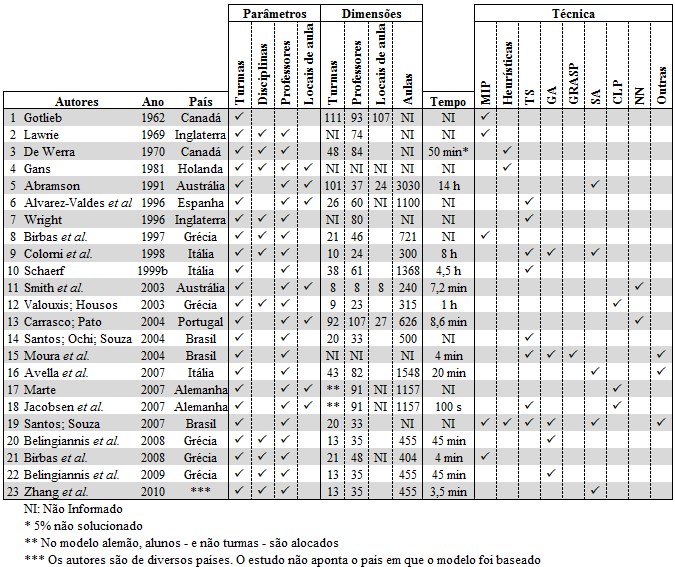
\includegraphics[angle=0,scale=1]{files/img/tabelas/Desenvolvimento.png}
    \legend{Fonte: \cite{alegre_desenvolvimento_2012}}
\end{figure}    % Desenvolvimento

Na figura \ref{University}, \cite{arratia-martinez_university_2021}, apresenta uma comparação similar à anterior, porém não separada em categorias, apenas categorizando entre verdadeiro e falso algumas características como alocação de salas, professores, nível institucional e método exato ou inexato.

% ![Comparação entre artigos que solucionam o problema de grade horária](img/tabelas/University.png)

\begin{figure}[htbp]\centering
    \caption{\label{University}Comparação entre artigos que solucionam o problema de grade horária}
    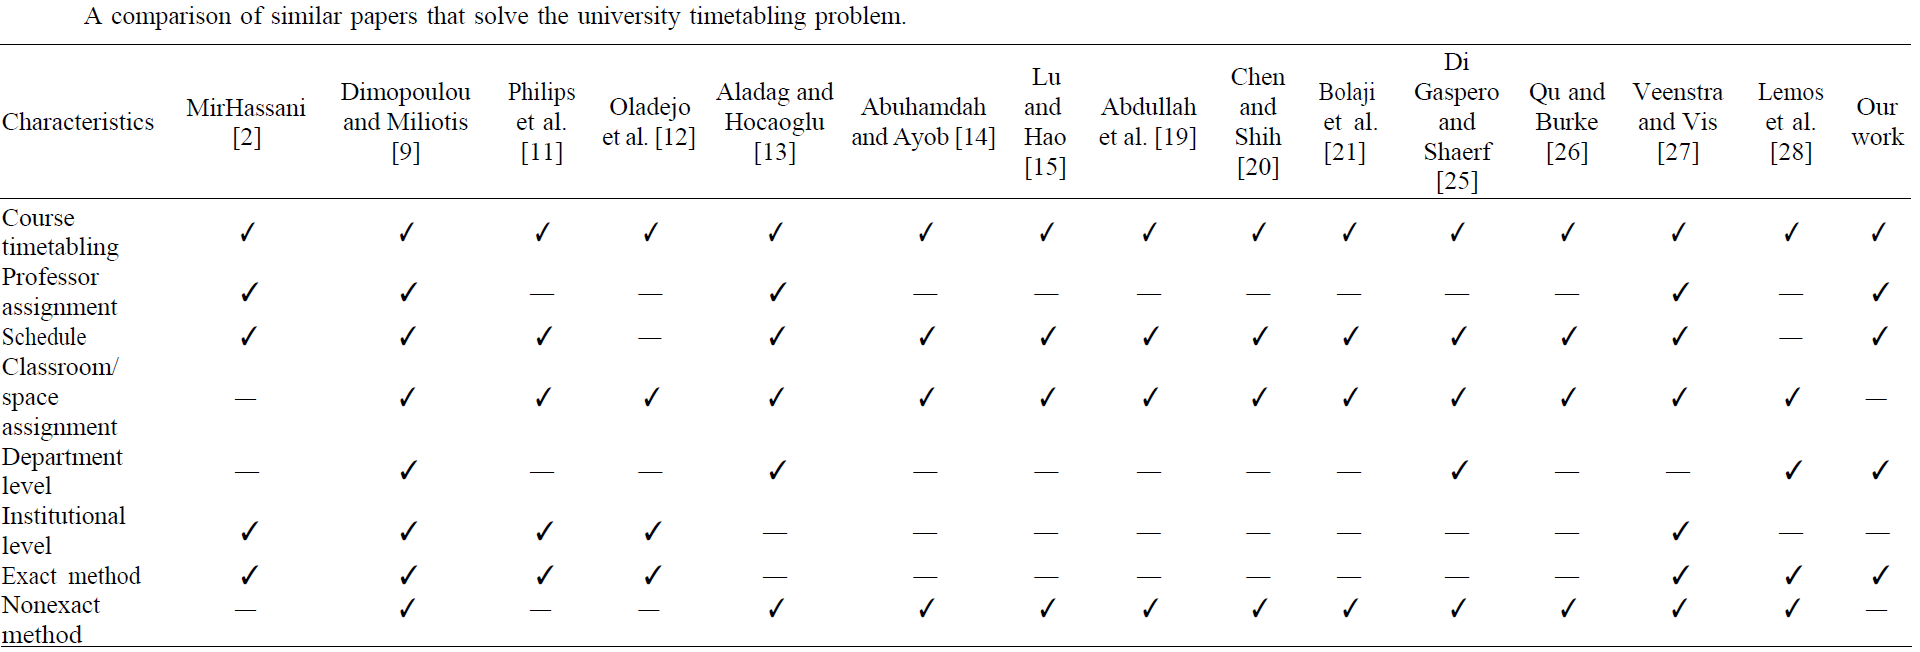
\includegraphics[angle=0,scale=0.37]{files/img/tabelas/University.png}
    \legend{Fonte: \cite{arratia-martinez_university_2021} - editado}
\end{figure}    % University

Na figura \ref{Visualization}, \cite{alencar_visualization_2019} explora uma categoria mais específica do problema, que é a característica da interatividade das interfaces desenvolvidas. Este apresenta características qualitativas quanto aos métodos, os dados dispostos, as técnicas de interação e o método utilizado para solucionar o problema de grade horária educacional. Nesta figura, os autores usam "Y" para simbolizar "Sim", "N" para "Não" e "-" para "Inconclusivo".

% ![Análise de publicações aceitas.](img/tabelas/Visualization.png)

\begin{figure}[htbp]\centering
    \caption{\label{Visualization}Análise de publicações aceitas.}
    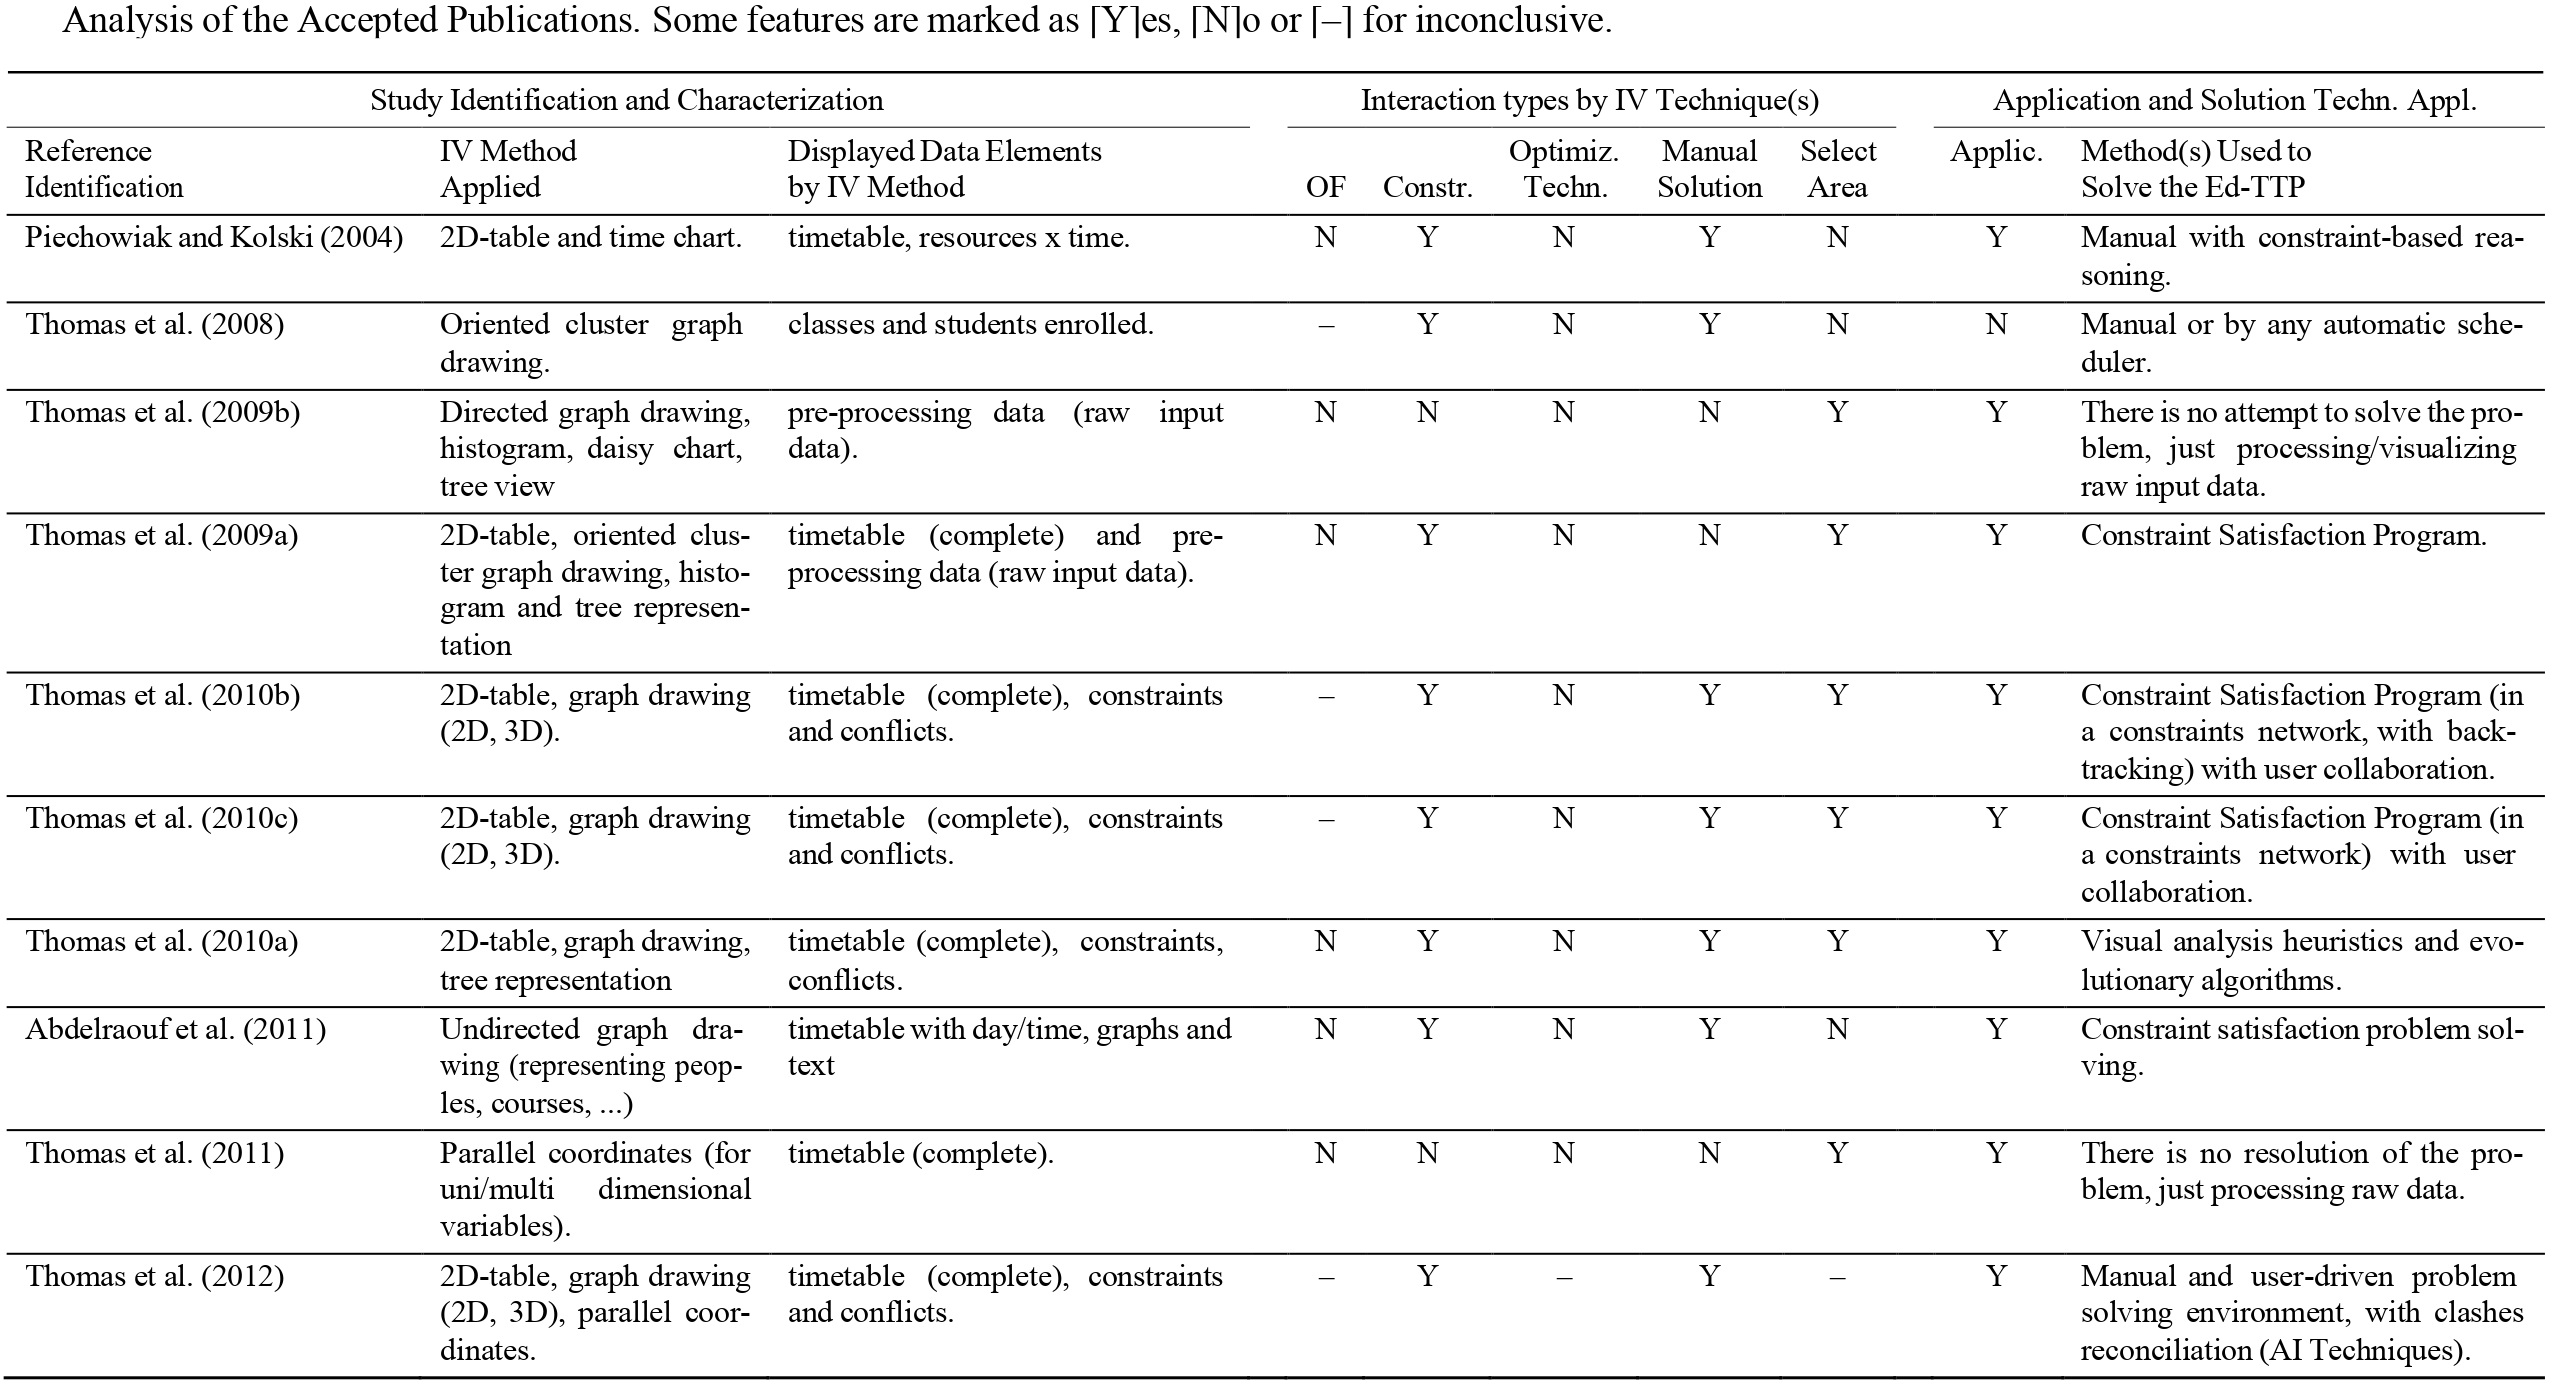
\includegraphics[angle=0,scale=0.7]{files/img/tabelas/Visualization.png}
    \legend{Fonte: \cite{alencar_visualization_2019} - editado}
\end{figure}    % Visualization

\section{ Desafios recorrentes} % ### 2.3. Desafios recorrentes

Apesar da vasta quantidade de trabalhos realizados com este fim, o \textit{Timetabling Problem} segue sendo uma área sem uma solução definitiva.

Tomáš Müller \cite{burke_modeling_2007} traz a questão da modelagem como um dos maiores obstáculos. À medida em que a complexidade aumenta, se torna cada vez mais difícil desenvolver uma solução efetiva. Assim fazendo com que a solução para uma universidade possa não ter utilidade para outras, ou até mesmo não seja capaz de lidar com todos os problemas de uma mesma universidade.

Apesar do contrafluxo encontrado na resolução desse problema, Tomáš cita que, apesar da complexidade, é sim possível desenvolver soluções que tenham uso prático, mesmo que não seja um processo fácil. As ferramentas existem e estão disponíveis. Restando então considerar e resolver as preocupações dos usuários às questões, visto que as técnicas de resolução já se encontram vastamente documentados.

Com isso, entramos também no ramo da Interação Homem-Máquina, ramo abordado por Dinata \cite{andre_interaction_2018} que visou em seu desenvolvimento a criação de uma interface focada no usuário. Assim minimizando o atrito na abordagem desse problema complexo. Também sendo área de enfoque de \cite{alencar_visualization_2019} em sua revisão literária

% <!--
% ### 2.5. Contexto histórico e origem

% - Como surgiu essa área? Em que momento ela se dividiu? Devo falar sobre isso?

% ### 2.6. Técnicas existentes(?)

% - Falar sobre técnicas existentes e quem já fez. Tipo o que aquele artigo sem DOI fez
% -->

\section{ Trabalhos anteriores} % ### 2.4. Trabalhos anteriores

Este trabalho não se mostra desprovido de histórico na tentativa de resolução do mesmo problema. Sânya e Ricardo, ambos estudantes de Ciência da Computação da UENF, já realizaram trabalhos com o mesmo fim, porém com abordagens diferentes da atual proposta.

Tendo vista que atualmente o problema de Programação Horária da UENF ainda perdura, podemos considerar que embora os trabalhos anteriores tenham se mostrado importantes ao pavimentar o caminho em direção à resolução da problemática disposta, as soluções ótimas encontradas por ambos, embora ótimas para a modelagem proposta, não se mostraram ótimas para a realidade da universidade.

Abaixo são listados os trabalhos anteriores e suas respectivas abordagens, bem como os apontamentos do que se mostrou inviável para a realidade da universidade.

\subsection{Sânya} % #### 2.4.1. Sânya

Em seu trabalho, Sânya aborda o problema de Programação de Horários de Disciplinas em Universidades, tendo como foco o curso de Ciência da Computação da UENF. Sua abordagem foi a de desenvolver um software que fosse capaz de gerar uma grade horária ótima para o curso, levando em conta as restrições impostas pelo curso. Para isso, Sânya explicou diversos métodos possíveis para se alcançar a solução desejada, passando inicialmente pelos métodos construtivos, seguido de métodos refinamento, podendo essas heurísticas serem utilizadas em conjunto com meta-heurísticas.

Por fim, utilizou uma heurística que consistia em respeitar a uma matriz de preferência para a distribuição das disciplinas. Seguindo com o uso do _Simulated Annealing_ para a otimização da solução inicial.

\subsection{Ricardo} % #### 2.4.2. Ricardo

- Contato dele
- Turma vs aluno
- Fixo vs solto
- Um professor por disciplina
- Uma turma por disciplina
- Disciplinas de um mesmo período não conflitando
- Dois horários de aula no mesmo dia: hard x soft
- Tamanha eficiência é de fato necessária?

> Como possível trabalho futuro propõe-se o aperfeiçoamento da interface gráfica e do banco de dados da ferramenta desenvolvida para que seja possível armazenar um maior número de informações pertinentes ao problema de uma forma eficiente, para que o usuário possa realizar modificações no quadro de horários e a ferramenta seja capaz de informar se essas modificações são viáveis ou não e para que a escolha dos dados usados na resolução do problema tenha uma maior flexibilidade. Além disso, os mecanismos usados na implementação da Função Objetivo (função que avalia a qualidade das soluções obtidas) podem ser aperfeiçoados com o intuito de cada vez mais atender a um maior número de particularidades do dia a dia do curso de Ciência da Computação da UENF.

\subsection{Divergências} % #### 2.4.3. Divergências

\subsubsection{Sânya} % ##### Sânya

É dito por Sânya que:

> Como na UENF a tarefa de distribuição de sala não varia muito a cada período, sendo feito separadamente por cada centro [...]

Embora possamos entender o conceito de "variar muito" como subjetivo, considerando que mesmo ao longo de um mesmo semestre existem realocações de salas e professores dentro do contexto de um mesmo Centro, podemos entender que a realidade da UENF é de fato muito dinâmica, não se encaixando completamente na solução de alocação única inicial de salas e professores.

Pode-se alegar que tratar da variabilidade de alocações de salas de um mesmo Centro foge do escopo do trabalho, porém, para que o coordenador da Computação tenha fácil acesso aos dados de alocação de salas disponíveis, faz-se necessário que seu uso esteja compartilhado com o Diretor do Centro de Ciência e Tecnologia (CCT), visto que este é o responsável pela alocação de salas de todos os cursos do CCT.

> [...] e as aulas que necessitam de salas com recursos especiais são geralmente já preestabelecidas, não há necessidade de automatizar esta tarefa de distribuição de salas.

Algumas turmas são historicamente alocadas à determinadas salas, mas isso não significa necessariamente que esta alocação é a mais adequada para a mesma. Então, todas as salas, mesmo que inicialmente pré-estabelecidas, devem estar passíveis de mudanças, mas com possibilidade de se fixar.

> Outra tarefa que no presente cenário do curso de Ciência da Computação não viabiliza algum tipo de automatização é a distribuição de professores, pois além de um número muito pequeno destes, não há muitas alternativas de mudanças de suas respectivas disciplinas.

Quanto à distribuição de professores, a realidade do curso de Ciência da Computação segue a mesma da que foi apontada em 2013 por Sânya. Entretanto, cada professor tem sua própria gama de disciplinas que se dispõe a ministrar, e a coordenação tende a distribuí-los de acordo com sua preferência. Entretanto, como a demanda dos alunos não se mostra linear como foi estudado, é possível que a distribuição de professores seja feita de forma mais eficiente, considerando a demanda dos alunos, ainda que não se descartem suas preferências pessoais.

> Requisitos essenciais, ou seja, obrigatórios:
>
> RE1 - Um professor não pode lecionar aula em duas turmas diferentes no mesmo horário.
> RE2 - Uma turma não pode ter aula em duas disciplinas no mesmo horário.
>
> Requisitos não essenciais, de qualidade:
>
> RNE1 - O ideal é que existam no máximo duas aulas consecutivas da mesma disciplina.
> RNE2 - Não devem haver mais de duas aulas da mesma disciplina em um dia.
> RNE3 - Não preencher os horários de 12h às 14h, pois se trata de horário de almoço.
> RNE4 - Os professores associados, por terem exclusividade com a instituição, preferem espalhar os horários das aulas dadas, e não acumular todas no mesmo dia.
> RNE5 - Os professores contratados, por outro lado, preferem que suas aulas sejam alocadas num mesmo dia, ou no menor número de dias possíveis.

Quanto à citada RE2, a limitação deveria ser mais criteriosa, e se tratando de um requisito não essencial, pois, o conceito de turma é dado pela junção de estudantes que cursam a mesma disciplina, ministrada por um mesmo professor, em um mesmo semestre. Mas em seu trabalho, Sânya considera o conceito de turma como sendo o conjunto de estudantes que ingressaram em um mesmo ano, independente da consideração da existência de repetentes e de suas escolhas pessoais de inscrição.

RNE1, RNE2 e RNE3: todas elas não consideram a existência de disciplinas que necessitam de um total de cinco tempos de aula semanais, sendo elas regularmente divididas em dois períodos, um de duas horas e outro de três horas. Que, em situações de necessidades, como é visto na entrevista com o diretor do CCT, acaba sim sendo necessário que se aloque em período de almoço.

RNE4 e RNE5: embora estejam direcionadas corretamente, ainda assim não engloba casos de preferência pessoal de cada um dos professores citados. Como por exemplo a possibilidade de não se ministrar aulas em determinados dias da semana por motivos religiosos, seja por parte do quadro permanente, quanto de professores associados.

Outra considerável divergência entre o modelo e a realidade é a definição de que a cada semestre contém apenas 5 turmas de computação. Sendo estas compostas pelos estudantes ingressantes de 5 anos consecutivos, caso este que não se aplica à realidade da universidade, visto que a quantidade de turmas varia de acordo com a demanda semestral, que não necessariamente condiz com todos os estudantes ingressantes de um mesmo ano.


% \chapter[Estrutura organizacional da UENF]{Estrutura organizacional da instituição estudada} % ## 4. Estrutura organizacional da instituição estudada

Para que se possa entender melhor o problema, é necessário que se entenda a estrutura organizacional da UENF disposta no \href{https://www.uenf.br/UENF_ARQUIVOS/Downloads/REITORIA_1360_1101117875.pdf}{Estatuto da UENF}. A \href{https://uenf.br/portal/}{Universidade Estadual do Norte Fluminense Darcy Ribeiro (UENF)}, ainda que limitando ao que convém neste trabalho.

\section{A UENF e seu estatuto} % ### 4.1. A UENF e seu estatuto     % Adicionar links corretos nos laboratórios e centros

% <!-- Provavelmente eu deveria adicionar informações sobre a secretaria acadêmica -->
% <!-- Precisa de revisão -->
% <!-- Sinto que falta falar sobre secretaria acadêmica e Conselho de Centro -->

Segundo o estatuto, a UENF compreende:

\begin{itemize}
  \item Órgãos da Administração Superior de política, gestão e supervisão;
  \item Unidades universitárias de ensino, pesquisa e extensão;
  \item Órgãos e serviços especiais, destinados a auxiliar na administração e a suplementar as atividades de ensino, pesquisa, extensão e apoio técnico.
\end{itemize}

% - Órgãos da Administração Superior de política, gestão e supervisão;
% - Unidades universitárias de ensino, pesquisa e extensão;
% - Órgãos e serviços especiais, destinados a auxiliar na administração e a suplementar as atividades de ensino, pesquisa, extensão e apoio técnico.

Quanto aos órgãos da Administração Superior devemos enfocar o órgão executivo, constituído unicamente pela reitoria, cujos órgãos auxiliares englobam a Secretaria Acadêmica, que por sua vez tem como algumas de suas atribuições as seguintes:

\begin{enumerate}
  \item Coordenar a \textbf{divulgação do horário escolar dos vários cursos da UENF}, de modo a \textbf{otimizar os recursos humanos}, \textbf{ampliar as opções de disciplinas para os alunos} e tornar acessíveis os dados escolares;
  \item \textbf{Centralizar os serviços de registro da vida escolar dos alunos}, compreendendo \textbf{inscrição}, admissão, \textbf{matrícula}, \textbf{créditos}, \textbf{opções}, transferências, promoções, graduações e preparação dos respectivos diplomas, dentro das normas estabelecidas.
\end{enumerate}

Já quanto as unidades universitárias de ensino, temos no estatuto que "as unidades universitárias de ensino, pesquisa e extensão, definidas por áreas de conhecimento, são constituídas em Centros, que por sua vez congregam Laboratórios afins" e que "o Laboratório é a menor parte da estrutura universitária para todos os efeitos de organização administrativa, didático-científica, distribuição de pessoal e de representação nos órgãos colegiados da UENF".

A administração do Centro é da competência do Diretor e seu Conselho. Os Laboratórios, por sua vez, são administrados pelos Chefes de Laboratório.

O Conselho de Centro, tem como uma de suas atribuições, descrito no inciso XVII do artigo 34 do estatuto, a seguinte: \textbf{designar, semestralmente, os professores responsáveis pelas disciplinas dos Cursos de Graduação} e Programas de Pós-Graduação, ouvidos os respectivos Laboratórios, os Colegiados de Curso e Comissões de Coordenação.

Atualmente, segundo o site da UENF, a universidade possui 4 Centros, sendo eles:

\begin{enumerate}
  \item Centro de Ciências do Homem - \href{https://uenf.br/}{CCH};
  \item Centro de Ciência e Tecnologia - \href{https://uenf.br/cct/}{CCT};
  \item Centro de Biociências e Biotecnologia - \href{https://uenf.br/}{CBB};
  \item Centro de Ciências e Tecnologias Agropecuárias - \href{https://uenf.br/}{CCTA}.
\end{enumerate}

E também existem 8 laboratórios vinculados ao Centro de Ciência e Tecnologia (CCT) possui 8 laboratórios, sendo eles:

\begin{enumerate}
  \item Laboratório de Meteorologia – \href{https://uenf.br/cct/administracao/laboratorios/}{LAMET};
  \item Laboratório de Ciências Físicas – \href{https://uenf.br/cct/lcmat/}{LCFIS};
  \item Laboratório de Engenharia Civil – \href{https://uenf.br/cct/administracao/laboratorios/}{LECIV};
  \item Laboratório de Ciências Químicas – \href{https://uenf.br/cct/administracao/laboratorios/}{LCQUI};
  \item Laboratório de Materiais Avançados – \href{https://uenf.br/cct/administracao/laboratorios/}{LAMAV};
  \item Laboratório de Ciências Matemáticas – \href{https://uenf.br/cct/administracao/laboratorios/}{LCMAT};
  \item Laboratório de Engenharia de Produção – \href{https://uenf.br/cct/administracao/laboratorios/}{LEPROD};
  \item Laboratório de Engenharia e Exploração de Petróleo – \href{https://uenf.br/cct/administracao/laboratorios/}{LENEP}.
\end{enumerate}

Os Laboratórios englobam os Cursos de Graduação e Pós-Graduação, que são administrados pelos Coordenadores de Curso.

Além disso, o LCMAT mantém dois cursos de graduação e um programa de pós-graduação stricto sensu. Sendo eles:

\begin{enumerate}
  \item \href{https://uenf.br/posgraduacao/licenciatura-matematica/}{Licenciatura em Matemática};
  \item \href{https://cc.uenf.br/}{Bacharelado em Ciência da Computação};
  \item \href{https://uenf.br/posgraduacao/matematica/apresentacao/}{Mestrado Profissional em Matemática} – \href{https://uenf.br/posgraduacao/programas/pos-graduacao-stricto-sensu/}{PROFMAT} / \href{https://www.profmat-sbm.org.br/}{SBM}.
\end{enumerate}

\section{Entrevistas} % ### 4.2. Entrevistas

% <!-- Separar entrevists de minhas opiniões pessoais -->

Como forma de entender melhor a percepção real daqueles que recorrentemente lidam com a tarefa de criação da grade horária, diversas entrevistas foram feitas com o intuito de analisar qualitativamente quais são as opiniões, pedidos, reclamações e pensamentos de diferentes níveis organizacionais da UENF.

\subsection{Diretor do CCT} % #### 4.2.1. Diretor do CCT

% <!-- Devo omitir o nome dos entrevistados? -->

O primeiro entrevistado foi o atual Diretor do CCT. Ele atualmente estrutura a relação de disciplinas ofertadas pelo CCT em Excel e as publica \href{https://uenf.br/cct/secretaria-academica/distribuicao-das-salas-de-aula-do-cct/}{em formato PDF no site do CCT}. Seu trabalho auxilia os Chefes de Laboratório e Coordenadores de Curso a visualizarem quais são as salas disponíveis e em quais horários cada professor está alocado.

Um dos tópicos dialogados, foi quanto às categorias das disciplinas, ou seja, quais características notáveis as disciplinas poderiam ter. Com isso podemos listar as seguintes categorias de disciplinas:

\begin{itemize}
  \item \textbf{Anuais}: disciplinas que ocorrem apenas uma vez no ano;
  \item \textbf{Ímpares}: disciplinas que são ofertadas no primeiro semestre letivo;
  \item \textbf{Pares}: disciplinas que são ofertadas no segundo semestre letivo;
  \item \textbf{De serviço}: disciplinas ofertadas para mais de um curso simultaneamente;
  \item \textbf{Ciclo básico}: disciplinas oferecidas para todas as engenharias;
  \item \textbf{Repetentes}: turmas criadas especialmente para repetentes.
\end{itemize}

% - Anuais: disciplinas que ocorrem apenas uma vez no ano;
% - Ímpares: disciplinas que são ofertadas no primeiro semestre letivo;
% - Pares: disciplinas que são ofertadas no segundo semestre letivo;
% - De serviço: disciplinas ofertadas para mais de um curso simultaneamente;
% - Ciclo básico: disciplinas oferecidas para todas as engenharias;
% - Repetentes: turmas criadas especialmente para repetentes.

As disciplinas ímpares e pares geralmente estão atreladas à expectativa de que os alunos progredirão sequencialmente sem reprovação alguma. Entretanto, caso uma quantidade de alunos considerável de alunos reprove em determinada disciplina, é possível que estes se enquadrem na criação de uma turma especial para repetentes, ou não.

Uma sugestão de utilidade para o software é a de permitir que as "disciplinas de serviço" sejam fixas, visto que estas são as que têm maior complexidade de manejamento de horário posteriormente, justamente por geralmente abrangerem muitos alunos e de diversos cursos diferentes.

Uma outra característica notável é a repetição de atribuições de disciplinas em pares regulares, ou seja, alocadas no mesmo período de horário com um dia de intervalo entre elas. Um exemplo desse tipo de alocação recorrente seria "14 às 16 horas de segunda e quarta feira".

Com isso, surge a dúvida: há uma preferência ativa por aulas alocadas com este padrão? A resposta dada é que não. O que se mostra como uma restrição a menos na hora de se alocar as turmas.

Outro caso notável é a existência majoritárias de turmas criadas com dois períodos de duas horas, entretanto existem algumas que fogem deste padrão e possuem três horas de duração. A solução encontrada pelo Diretor é a de colocar esta disciplina começando às 10h, o que faz com que se alongue até as 13h, período geralmente usado pelos estudantes e servidores para se alimentar, e justamente por isso evitando que atrapalhe a distribuição das salas. Outra alternativa é alocar esta turma para as 13h, fazendo com que finalize às 16h, horário em que as disciplinas com duas horas de duração geralmente terminam.

Segundo ele, saber a demanda máxima possível seria bom, visto que podem haver casos de solicitações de vagas para disciplinas de serviço que extrapolam a quantidade esperada para a distribuição balanceada dentre os cursos.

Uma outra situação que ocorre é que algumas disciplinas historicamente têm seus horários definidos em um mesmo horário ao longo dos anos. Caso essa alocação seja alterada, ocorre a possibilidade de reclamação por parte dos professores, mesmo que esta alteração seja benéfica para os estudantes. Então por exemplo, os horários de 8h de uma segunda feira e de 16h de sexta feira, não são geralmente desejados pelos professores, mesmo que eles teoricamente tenham disponibilidade de 8 horas diárias.

Considerando a quantidade de laboratórios "concorrendo" simultaneamente às vagas, surge a dúvida: há ordem de precedência entre os laboratórios? A resposta para esta pergunta é "Não. As vagas são distribuídas com prioridade na ordem de chegada".

Algumas outras informações que ele elenca:

\begin{itemize}
  \item Os períodos ímpares são os piores;
  \item Essa opinião pode ser resultado do fato de que os períodos ímpares apresentam um intervalo de tempo para preparo das grades menor do que os períodos pares;
  \item As disciplinas básicas são grandes;
  \item É esperado que uma grande quantidade de alunos se inscreva nas disciplinas essenciais e iniciais de seus cursos, sendo boa parte dela relacionada com o conceito das disciplinas de serviço e com o conceito de ciclo básico das engenharias;
  \item As disciplinas de serviço devem ser alocadas primeiro;
  \item Visto a grande quantidade de conflitos possíveis dentre os diversos cursos, ao alocá-las primeiro, os conflitos passam a ocorrer em turmas com uma quantidade menor de pessoas e/ou que sejam de um mesmo curso;
  \item As alterações vão até o final do período;
  \item Embora possa parecer que a alocação de turmas finalize após o encerramento do período de inscrição e desinscrição, na prática, a realocação ocorre durante todo o período;
  \item Teoricamente matérias de um mesmo período não devem conflitar;
  \item Isso se dá segundo a percepção de que a maioria dos alunos está seguindo a mesma linha sequencial de disciplinas, o que muitas das vezes não é a realidade.
\end{itemize}

\subsection{Desenvolvedor do Sistema Acadêmico} % #### 4.2.2. Desenvolvedor do Sistema Acadêmico

Considerando que a integração do sistema proposto seria certamente mais eficiente se integrada ao sistema acadêmico, viu-se como apropriado entrevistar o desenvolvedor do Sistema Acadêmico para se ponderar sobre o uso dos dados e a possível integração.

Durante a entrevista, foram listados alguns dados que seriam interessantes para a análise, sendo eles a demanda de disciplinas, a listagem dos professores, a listagem dos alunos aprovados e suas respectivas disciplinas e por fim os requisitos das disciplinas.

% - Demanda de disciplinas
% - Listagem de professores
% - Listagem dos alunos aprovados
% - Requisitos das disciplinas

Outra questão analisada seria quanto a forma de integração. Boa parte das aplicações web se comunicam em forma de API, entretanto, devido à quantidade de alterações executadas ao longo do semestre no sistema acadêmico, o Desenvolvedor do Sistema Acadêmico utiliza o sistema de mensagerias através do \href{https://www.rabbitmq.com/}{RabbitMQ}.

Foi citado sobre a abordagem do Coordenador de Computação para o cálculo das demandas, quanto a isso, o Desenvolvedor citou que poderia facilmente permitir o download de um CSV dos dados necessários.

Quanto à possibilidade de aprimoramentos no Sistema Acadêmico, ele disse que "eu faço o que me pedem", se referindo ao repositório do Acadêmico disponível no \href{https://about.gitlab.com/}{GitLab}, onde alguns poucos usuários fazem solicitações de alterações e melhorias. Havendo então a possibilidade de que o Coordenador de Computação faça uma solicitação à SECACAD para que seja implementada uma funcionalidade que permita a exportação dos dados necessários para o cálculo das demandas.

Um outro problema apontado por ele é a falta de gente. Segundo ele, outras duas pessoas entraram junto com ele no mesmo concurso, mas foram realocadas para outras áreas da universidade. Ele cita também sobre a "cultura do trabalho opcional" existente na UENF, onde muitos servidores não se sentem obrigados a trabalhar.

Em relação a estrutura dos dados, o sistema acadêmico utiliza o SQL. Foi citado o uso de NOSQL e estrutura de Grafos como possibilidades de mudança, mas como a mesma não se mostrou necessária até o momento, não foi implementada.

Uma questão levantada pelo entrevistado diz respeito à manutenção do software desenvolvido neste trabalho. Não sabendo ele dizer se o mesmo seria mantido pela UENF.

Ele também sugere que, para evitar a complexidade de se trabalhar com dados reais de alunos, que sejam utilizados dados fictícios.

\subsection{Chefe de Laboratório de Matemática} % #### 4.2.3. Chefe de Laboratório de Matemática

Considerando que um dos cargos relacionados com o processo de elaboração de grades horários é o de Chefe de Laboratório, foi entrevistada a atual Chefe de Laboratório de Matemática.

Assim como sugerido pelo Desenvolvedor do Sistema Acadêmico, a Chefe também sugeriu que dados fictícios fossem utilizados. Sugeriu ainda que fosse utilizado o schema do banco de dados do sistema acadêmico como sua criação. Outra sugestão foi a solicitação ao Desenvolvedor do Sistema Acadêmico uma listagem de possíveis valores recorrentes no banco de dados.

A entrevistada também relatou algumas problemáticas envolvendo a realocação dos horários das turmas. Segundo ela, qualquer alteração pode ser feita durante a semana anterior à matrícula, visto que, não havendo inscritos, não há problema na alteração. A partir do momento em que houver ao menos um aluno inscrito na disciplina, alterações só podem ser feitas caso não haja conflitos aparentes e preferencialmente com um documento assinado pelos alunos que estiverem inscritos.

\subsection{Responsável pela Secretaria Acadêmica (SECACAD)} % #### 4.2.4. Responsável pela Secretaria Acadêmica (SECACAD)

Inicialmente, alguns tópicos foram trazidos como ponto focal da entrevista, sendo alguns deles os seguintes:

\begin{itemize}
  \item Dúvidas quanto as atribuições da SECACAD;
  \item Permissão de acesso aos dados que não são estritamente necessários, mas ajudariam;
  \item Definição dos períodos, demanda provisória e erros de estimativa;
  \item GitLab, tarefas (issues) e demandas;
  \item Automatização da burocracia;
  \item Ética VS Eficiência.
\end{itemize}

% - Dúvidas quanto as atribuições da SECACAD
% - Permissão de acesso aos dados que não são estritamente necessários, mas ajudariam
% - Definição dos períodos, demanda provisória e erros de estimativa
% - GitLab, tarefas (issues) e demandas
% - Automatização da burocracia
% - Ética VS Eficiência

Logo de início, o entrevistado informou que ele não pode ceder dados de nenhum aluno, mesmo que anonimizados, mas sugeriu que poderia reencaminhar um formulário de pesquisa para os alunos, para que assim eles próprios pudessem fornecer os dados necessários.

Outra abordagem interessante informada por ele é quanto ao seu conhecimento técnico, onde sugeriu abordagens de análise multicritérios como forma de se auxiliar a criação das grades horárias.

Durante a conversa, foi citado de forma positiva quanto à demanda exata de cada disciplina. Reforçou-se a preferência pela alocação de disciplinas visando os estudantes mais próximos da conclusão do curso, estando em último na ordem de prioridade aqueles que decidem se adiantar com disciplinas de períodos mais avançados. Uma outra característica apontada é que a sequência de definições é a seguinte: Vagas $\rightarrow$ Professor $\rightarrow$ Sala $\rightarrow$ Horário.

Também se confirmou a não existência de um registro oficial das salas e suas capacidades. Essa informação é inserida como um campo de texto no sistema acadêmico, com isso, o sistema não impediria a alocação de duas turmas em uma mesma sala em um mesmo horário.

O responsável pela SECACAD também informou que cabe à Pró-Reitoria a mudança do início do primeiro semestre para expandir o período de preparação das grades horárias para o segundo período, sendo que este pedido deve partir da Câmara de Graduação.

Quanto ao tópico "ética VS eficiência", ele citou que embora o sistema acadêmico impeça a realocação de turmas com alunos inscritos, é possível que o mesmo seja burlado ao manualmente se excluir a inscrição do aluno. Sendo esta prática justificável em alguns casos.

Uma ferramenta que o beneficiaria seria a análise dos alunos que estão à beira de perder o vínculo com a universidade, para que a Secretaria Acadêmica possa tomar as medidas cabíveis.

\subsection{Coordenador de Computação} % #### 4.2.5. Coordenador de Computação

Sendo o Coordenador de Computação o principal usuário do sistema, torna-se imprescindível a análise qualitativa de sua perspectiva.

Seguindo o conceito de Design Iterativo utilizado também por \cite{andre_interaction_2018}, o Coordenador foi consultado em diversas etapas do desenvolvimento do sistema. Inicialmente, foi apresentado a ele o conceito do sistema, suas funcionalidades e possíveis benefícios. Em seguida, foi apresentado a ele um protótipo do sistema. Mas esta questão será melhor tratada em outro segmento deste mesmo trabalho, aqui será abordado apenas o conteúdo das entrevistas.

Assim como comentado pelo Diretor do CCT, o Coordenador também fala sobre a definição de matérias que se mostram fixas, porém, agora com outro olhar: enquanto o diretor vê as matérias fixas como uma forma de atribuição histórica seguindo a ideia de "já era assim quando eu cheguei", o Coordenador por sua vez vê apenas como uma forma predefinida e imutável. Porém, olhando em um contexto mais amplo, essa definição de matérias não se mostra como obrigatória, visto que pode haver casos em que outra alocação de uma disciplina "fixa" apresente uma qualidade melhor do que seu horário usual.

Outra questão levantada por ele é quanto a um problema já antigo no curso de Ciência da Computação na UENF, que há anos apresenta um corpo docente reduzido em comparação com outros cursos, sendo necessário um desdobramento maior para suprir a demanda de disciplinas dos alunos. Uma solução utilizada é a de solicitar a abertura de uma bolsa para docência complementar, onde um aluno de pós-graduação pode ser alocado como professor de uma disciplina. Solução que embora não seja a ideal, é a que se mostra mais viável, dada a diminuta inscrição de candidatos à docência.

Uma outra característica até então não citada pelos outros entrevistados é que existem salas que são vistas culturalmente como sendo de determinado curso, onde acaba sendo um certo tabu a alocação de uma disciplina de outro curso, mesmo que não se esteja infringindo regra alguma.

Quanto à priorização de veteranos já citada anteriormente, o Coordenador aponta uma outra forma de se enxergar a situação: em disciplinas dos períodos finais do curso, a prioridade é dos veteranos, ficando os calouros que ocasionalmente possam ter se adiantado, em segundo plano. Já em disciplinas dos períodos iniciais, a prioridade é dos calouros, ficando os veteranos que por ventura tenham reprovado, em segundo plano.

Diferente de como foi respondido pelo Diretor do CCT, para o Coordenador de Computação a alocação de disciplinas em pares se mostra como "didática", sendo ela então preferível, mas não necessariamente vista como obrigatória.

Considerando a recorrência de citação do conceito de estimativas de demanda, o Coordenador de Computação sugere que haja um campo no sistema para que seja inserida a demanda estimada de cada disciplina.

Considerando que no contexto atual do curso de Ciência da Computação na UENF é iminente a adoção de uma nova grade curricular, o Coordenador apresentou preocupação em relação à possibilidade de que o sistema não seja mais utilizado após a adoção da nova grade. Essa questão encontra-se atualmente fora do escopo do atual projeto, entretanto, não se mostra como um problema de difícil solução, visto que o sistema pode ser adaptado para a nova grade.

\subsection{Entendimento geral das entrevistas} % #### 4.2.6. Entendimento geral das entrevistas

Podemos concluir após a análise qualitativa das entrevistas que há de fato um certo grau de insatisfação por parte dos usuários do sistema atual. Embora o sistema funcione, ele apresenta gargalos que poderiam ser resolvidos com a utilização de um sistema mais eficiente que envolvesse mais diferente as diferentes partes interessadas. Suas maiores insatisfações são quanto à burocracia e o curto período de tempo disposto para a elaboração das grades horárias.

Embora não sejam apontadas como insatisfação, algumas potenciais ferramentas e melhorias foram também citadas pelos entrevistados. Dentre elas, a demanda máxima possível, que passaria a evitar superestimações de demanda, a alocação de disciplinas de serviço como fixas, e em alguns casos, a alocação de disciplinas em pares, que embora não seja uma regra, é uma preferência de um dos entrevistados. Outra ferramenta que foi citada é a de análise de alunos à beira de perder o vínculo com a universidade, que poderia ser utilizada pela Secretaria Acadêmica para tomar as medidas cabíveis. Também se fazendo notória a necessidade de registro oficial das salas e suas capacidades, que atualmente é inserida como um campo de texto no sistema acadêmico.

Outros problemas encontrados, remetem à acomodação institucional de algumas práticas, como a alocação de disciplinas em horários fixos, em pares e/ou nas mesmas salas. Essas práticas, embora não sejam obrigatórias, são vistas como um costume e por isso são mantidas.

\section{Sequência de criação das grades horárias} % ### 4.3. Progressão usual da criação de grades horárias

% <!-- Estou com dúvida novamente de qual é a progressão e de quem faz o quê -->

Ao somarmos o conhecimento presente no estatuto da UENF, com o conhecimento adquirido através das entrevistas, podemos ter uma visão geral de como se dá a criação das grades horárias na UENF. Assim, abaixo estão listados os passos que geralmente são seguidos para a criação das grades horárias.

% <!--
% Tendo obtido as informações dos \textit{stakeholders} primários, será então necessário modelar quais são as regras que ditam a estrutura organizacional em foco. Para este fim, serão utilizados diagramas conceituais utilizando softwares de suporte como o [Visual Paradigm][LinkVisualParadigm], [draw.io][LinkDrawio] e a [ferramenta Mermaid][LinkMermaid].
% Fazer um diagrama de... sei lá, aquele que tem barras retas. Diagrama de atividades?
% -->

\begin{enumerate}
  \item Período ocorrendo normalmente;
  \item Coordenadores enviam para Chefes de Laboratório uma demanda estimada de cada uma das disciplinas que serão ofertadas;
  \item Chefes de Laboratório atrelam professores a disciplinas;
  \item Chefes de Laboratório enviam para Diretores de Centro a demanda estimada;
  \item Dependendo das disponibilidades dos professores, cabe solicitar a abertura de uma bolsa de apoio ao ensino;
  \item O Diretor aloca provisoriamente as disciplinas em horários e salas;
  \item O Coordenador de Curso analisa possíveis mudanças de horários que possam ser mais eficientes na distribuição dos alunos;
  \item O período letivo acaba;
  \item Estima-se mais precisamente a demanda de cada disciplina;
  \item Turmas são abertas com a quantidade de vagas de acordo com as demandas estimadas;
  \item Alunos se inscrevem;
  \item Últimas mudanças são feitas;
  \item Período de inclusão e exclusão;
  \item Alguns possíveis ajustes finais;
  \item Período ocorrendo normalmente.
\end{enumerate}

% 1. Período ocorrendo normalmente;
% 2. Coordenadores enviam para Chefes de Laboratório uma demanda estimada de cada uma das disciplinas que serão ofertadas;
% 3. Chefes de Laboratório atrelam professores a disciplinas;
% 4. Chefes de Laboratório enviam para Diretores de Centro a demanda estimada;
% 5. Dependendo das disponibilidades dos professores, cabe solicitar a abertura de uma bolsa de apoio ao ensino;
% 6. O Diretor aloca provisoriamente as disciplinas em horários e salas;
% 7. O Coordenador de Curso analisa possíveis mudanças de horários que possam ser mais eficientes na distribuição dos alunos;
% 8. O período letivo acaba;
% 9. Estima-se mais precisamente a demanda de cada disciplina;
% 10. Turmas são abertas com a quantidade de vagas de acordo com as demandas estimadas;
% 11. Alunos se inscrevem;
% 12. Últimas mudanças são feitas;
% 13. Período de inclusão e exclusão;
% 14. Alguns possíveis ajustes finais;
% 15. Período ocorrendo normalmente.

Entrando em detalhes ainda maiores, podemos citar uma das etapas de criação das grades horárias que é a coleta de uma demanda esperada. Nela, cada Coordenador elabora de seu próprio modo. Uma possibilidade seria analisar quantos alunos costumam reprovar em determinada disciplina pela visualização estatística anterior, somado aos que possivelmente aprovarão na disciplina que é pré-requisito. Porém, toda essa pesquisa e estimativa é dispendiosa e pode desagradar a alguns coordenadores, ou então gerar estimativas incondizentes com a realidade.

Entendemos então que dentro do contexto da universidade, o problema de agendamento se torna mais complexo pois um dos recursos que está relacionado com o problema é a existência de prazos em cada uma das etapas, assim fazendo com que uma solução ideal seja aquela que é capaz de ser executada dentro do prazo estipulado, mesmo que não seja ótima.

\section{Formulário de pesquisa} % ### 4.4. Formulário de pesquisa % Adicionar as imagens do formulário

% <!-- CORRIGIR FUTURAMENTE - XXX --> <!-- Checar se as perguntas nas tabelas, prints e anexo são as mesmas -->

Como forma de analisar também a perspectiva dos discentes quanto à problemática abordada, foi elaborado um formulário de pesquisa com o intuito de se confirmar ou não a hipótese de que em sua maioria os alunos também se encontram insatisfeitos com a atual conjuntura de distribuição e alocação de turmas.

Para este fim, foi utilizado um formulário de pesquisa qualitativa dos alunos disponível no Apêndice 1. O formulário foi divulgado através de um link disponibilizado no grupo de alunos do curso de Ciência da Computação no WhatsApp, e também através de um link distribuído pela Secretaria Acadêmica a discentes da UENF.

A seguir, estão dispostos alguns resultados obtidos pelo formulário.

\subsection{Respondentes} % #### 4.4.1. Respondentes

Inicialmente foi solicitadas algumas informações dos alunos, como seu curso, ano de ingresso. As respostas estão dispostas na Figura \ref{fig:2.0-SobreVoce}.

\begin{figure}[htbp]\centering
  \caption{\label{fig:2.0-SobreVoce}Perguntas sobre o curso e ano de ingresso dos estudantes}
  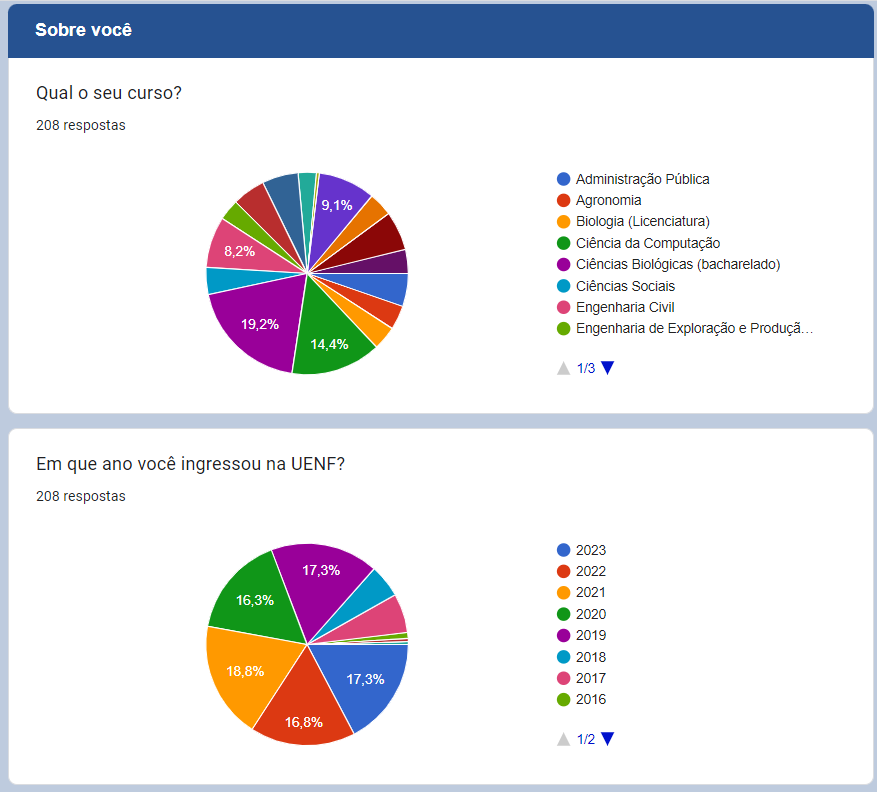
\includegraphics[scale=0.8]{files/img/Forms/2.0-SobreVoce.png}
  \legend{Fonte: o autor}
\end{figure} % SobreVoce

O formulário foi respondido por 208 alunos, sendo os cursos de maior incidência o bacharelado de Ciências Biológicas com 40 respondentes, Ciência da Computação com 29 e Medicina Veterinária com 19 (Tabela \ref{table:2.1_SobreVoce_Cursos}). Vale ressaltar que 96 dos respondentes são alunos de cursos que envolvem diretamente o CCT. Entretanto, a análise dos gráficos abordará a percepção de todos igualmente.

\begin{table}[htbp]
  \centering
  \caption{\label{table:2.1_SobreVoce_Cursos}Número de respondentes por curso}
  \begin{tabular}{| r l |}
    \hline
    \textbf{Quantidade} & \textbf{Curso}                                  \\
    \hline
    40                  & Ciências Biológicas (bacharelado)               \\
    29                  & Ciência da Computação                           \\
    19                  & Medicina Veterinária                            \\
    17                  & Engenharia Civil                                \\
    13                  & Química (Licenciatura)                          \\
    12                  & Engenharia Metalúrgica                          \\
    11                  & Engenharia de Produção                          \\
    11                  & Administração Pública                           \\
    9                   & Ciências Sociais                                \\
    8                   & Agronomia                                       \\
    8                   & Biologia (Licenciatura)                         \\
    8                   & Pedagogia (Licenciatura)                        \\
    8                   & Zootecnia                                       \\
    7                   & Engenharia de Exploração e Produção de Petróleo \\
    6                   & Física (licenciatura)                           \\
    1                   & Matemática (Licenciatura)                       \\
    0                   & Engenharia Meteorológica                        \\
    0                   & Outro                                           \\
    \hline
  \end{tabular}
\end{table}

Vemos também a distribuição dos anos de ingresso dos alunos que responderam o formulário, sendo seu quantitativo bem distribuído entre os anos de 2019 e 2023, tendo os anos de 2017 e 2018 uma quantidade menor de respostas, os outros anos tendo em conjunto um total de 4 respostas (Tabela \ref{table:2.2_SobreVoce_Anos}).

\begin{table}[htbp]
  \centering
  \caption{\label{table:2.2_SobreVoce_Anos}Número de respondentes por ano}
  \begin{tabular}{| c c |}
    \hline
    \textbf{Quantidade} & \textbf{Ano} \\
    \hline
    36                  & 2023         \\
    35                  & 2022         \\
    39                  & 2021         \\
    34                  & 2020         \\
    35                  & 2019         \\
    11                  & 2018         \\
    13                  & 2017         \\
    2                   & 2016         \\
    1                   & 2015         \\
    0                   & 2014         \\
    0                   & 2013         \\
    1                   & Outro        \\
    \hline
  \end{tabular}
\end{table}

\subsection{Avaliação de experiência acadêmica} % #### 4.4.2. Pesquisa de satisfação

Considerando que o escopo deste trabalho revolve em torno da alocação de recursos físicos e humanos, como salas, professores e alunos, foi elaborada uma seção do formulário de pesquisa com o intuito de se analisar a frequência de ocorrência de certas situações no contexto universitário. Para isto, foram feitas as seguintes perguntas:

\begin{enumerate}
  \item Salas: Você já teve que mudar de sala por falta de algum acessório como quadro, projetor ou monitor? % 53.1%
  \item Salas: Você já teve aula cuja sala não dispunha de carteiras o suficiente? % 52.7%
  \item Vagas: Você já quis entrar em uma disciplina, mas ela não tinha vaga? % 85.0%
  \item Vagas: Você já ficou acordado após meia-noite por medo de não ter vaga para as disciplinas que deseja cursar? % 91.3%
  \item Conflitos: Você já deixou de se inscrever em uma disciplina por causa de conflito de horário? % 90.8%
  \item Preferências: Você já preferiu não se inscrever em uma disciplina para cursá-la em outro momento mais oportuno? % 86.0%
  \item Opiniões: Você acha que a universidade deveria oferecer horários diferentes para as disciplinas mais demandadas para evitar conflitos com outras  % 100.0%
\end{enumerate}

A enumeração das perguntas feitas se encontra representada com suas respectivas respostas na Tabela \ref{table:3.0_satisfacao}.

\begin{table}[htbp]
  \centering
  \caption{\label{table:3.0_satisfacao}Ocorrência de experiências acadêmicas}
  \begin{tabular}{| c | c c c |}
    \hline
    \multicolumn{1}{|c|}{\multirow{2}{*}{Pergunta}} & \multicolumn{3}{c|}{Respostas}
    \\
    \multicolumn{1}{|c|}{}                          &
    Sim                                             &
    \multicolumn{1}{|c|}{Não}                       &
    Outro
    \\
    \hline
    1                                               & 110                            & 87 & 10 \\ % 110/207=0.5314 =  53.1%
    2                                               & 109                            & 95 & 3  \\ % 109/207=0.5265 =  52.7%
    3                                               & 176                            & 28 & 3  \\ % 176/207=0.8502 =  85.0%
    4                                               & 189                            & 17 & 1  \\ % 189/207=0.9130 =  91.3%
    5                                               & 188                            & 15 & 4  \\ % 188/207=0.9082 =  90.8%
    6                                               & 178                            & 27 & 2  \\ % 178/207=0.8599 =  86.0%
    7                                               & 207                            & 0  & 0  \\ % 207/207=1.0000 = 100.0%
    \hline
  \end{tabular}
\end{table}

As respostas respectivas às perguntas se encontram na Figura \ref{fig:3.0_Satisfacao} onde estão dispostos os resultados encontrados nesta seção.

\begin{figure}[htbp]\centering
  \caption{\label{fig:3.0_Satisfacao}Respostas sobre a satisfação dos estudantes}
  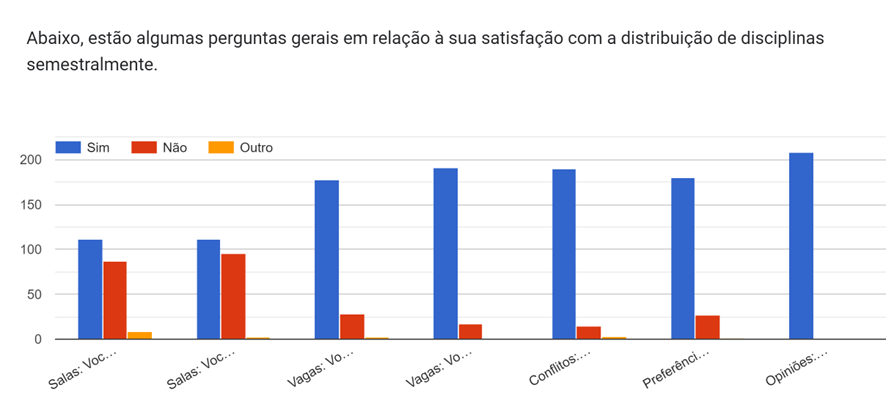
\includegraphics[scale=0.8]{files/img/Forms/3.0-Satisfacao.png}
  \legend{Fonte: o autor}
\end{figure} % Satisfacao

Quanto à distribuição dos recursos físicos, vemos uma taxa de 53,1\% de alunos que já tiveram que mudar de sala por falta de algum acessório disposto necessário para a aula. Já a necessidade de mudança de sala devido à ausência de carteiras suficientes obteve taxa de 52,7\%.

É notório o receio dos alunos quanto à possibilidade de não conseguir se inscrever nas disciplinas que desejam cursar, tendo sido confirmado por 85,0\% dos respondentes que se viram em situação em que a disciplina na qual desejavam se matricular não dispunha de vagas o bastante. Essa realidade resulta no temor por semestralmente não conseguir se inscrever na disciplina desejada, fazendo com que 91,3\% dos respondentes tenham se mantido acordados após a meia-noite por causa deste medo.

O temor de não conseguir se inscrever nas disciplinas desejadas é ainda agravado pelo fato de que 90,8\% dos alunos que já deixaram de se inscrever em disciplinas devido a conflitos de horário.

O que se apresenta como um agravante ainda maior na percepção da progressão não sequencial dos alunos é a quantidade de alunos que já preferiram não se inscrever em uma disciplina para cursá-la em outro momento mais oportuno, mesmo que isto signifique um atraso na progressão do curso, sendo seu percentual 86,0\%.

Embora seja uma prática recorrente a oferta de diversas turmas para uma mesma disciplina, o que usualmente é feito de forma que as turmas sejam ofertadas no mesmo horário. Entretanto, os alunos, unanimemente, não se mostram satisfeitos com esta prática, visto que 100\% dos respondentes consideram que a universidade deveria dispor de outros horários para as disciplinas mais demandadas com o intuito de evitar conflitos de horários.

Este resultado é curioso, visto que o temor de não se atrasar em seu progresso e conseguir se inscrever nas disciplinas desejadas, contrasta diretamente com a preferência pessoal de não se inscrever em disciplinas e cursá-las posteriormente, mesmo que isso possa atrasar seu progresso. Entende-se que nem todas as disciplinas, caso não cursadas em seu período esperado, resultarão no atraso da grade, mas ainda assim, a antítese é evidente.

\subsection{Preferências pessoais} % #### 4.4.3. Preferências pessoais

Neste segmento, visa-se entender um pouco melhor o processo decisório dos alunos quanto à escolha das disciplinas que desejam cursar. Primeiro, lhes é indagado quanto à disposição das disciplinas, variando entre disciplinas concentradas em poucos dias ou espalhadas durante a semana (Figura \ref{fig:4.1-PreferenciasPessoais-Distribuida_Acumulada}) e quanto à preferência de horários, variando entre horários matutinos e vespertinos (Figura \ref{fig:4.2-PreferenciasPessoais-Manha_Tarde}).

Embora não lide com conflitos, a análise de seus resultados pode auxiliar na escolha de distribuição futura dos usuários do sistema, ao desenvolverem a grade horária, caso desejem considerar as preferências dos estudantes.

\begin{figure}[htbp]\centering
  \caption{\label{fig:4.1-PreferenciasPessoais-Distribuida_Acumulada}Preferências por distribuição de disciplinas ao longo da semana}
  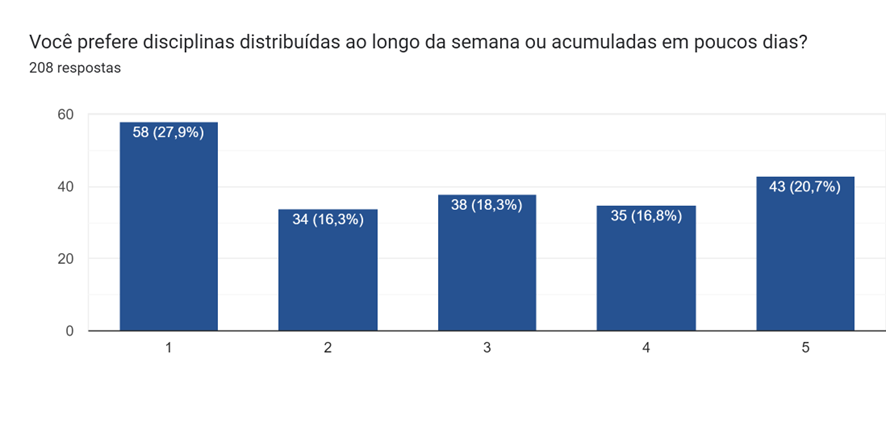
\includegraphics[scale=0.6]{files/img/Forms/4.1-PreferenciasPessoais-Distribuida_Acumulada.png}
  \legend{Fonte: o autor}
\end{figure} % PreferenciasPessoais Distribuida_Acumulada

\begin{figure}[htbp]\centering
  \caption{\label{fig:4.2-PreferenciasPessoais-Manha_Tarde}Preferências por distribuição de disciplinas em um mesmo dia}
  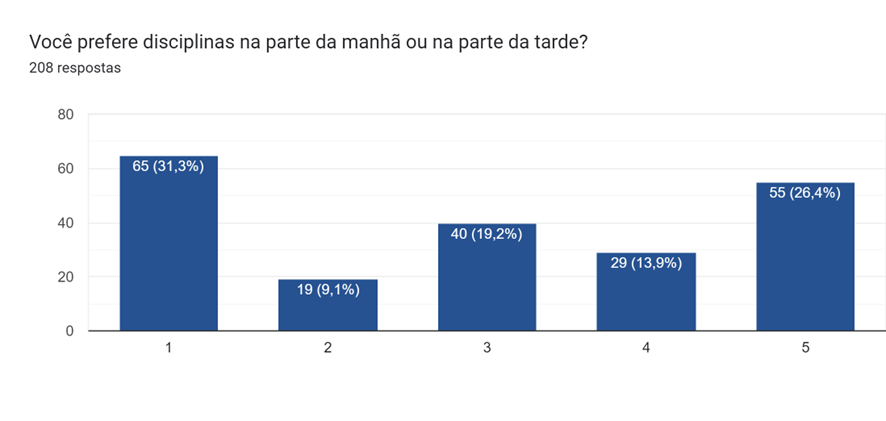
\includegraphics[scale=0.6]{files/img/Forms/4.2-PreferenciasPessoais-Manha_Tarde.png}
  \legend{Fonte: o autor}
\end{figure} % PreferenciasPessoais Manha_Tarde

Podemos ver na Figura \ref{fig:4.1-PreferenciasPessoais-Distribuida_Acumulada} que há uma grande distribuição entre as preferências dos alunos, tendendo às extremidades, onde alguns preferem bastante as disciplinas distribuídas ao longo da semana enquanto outros preferem disciplinas acumuladas em poucos dias, vindo como terceira opção mais votada a neutralidade. Observação similar se mostra presente também na Figura \ref{fig:4.2-PreferenciasPessoais-Manha_Tarde}.

Como alternativa de visualização, dispomos aqui das Tabela \ref{table:4.1-PreferenciasPessoais-Distribuída_Acumulada} e \ref{table:4.2-PreferenciasPessoais-Manha_Tarde} com os resultados numéricos.

\begin{table}[htbp]
  \centering
  \caption{\label{table:4.1-PreferenciasPessoais-Distribuída_Acumulada}Preferências por distribuição de disciplinas em um mesmo dia}
  \begin{tabular}{| r l |}
    \hline
    \textbf{Quantidade} & \textbf{Distribuição na semana} \\
    \hline
    58                  & Distribuídas ao longo da semana \\
    34                  & $\sim$                          \\
    38                  & Não tenho preferência           \\
    35                  & $\sim$                          \\
    42                  & Acumuladas em poucos dias       \\
    \hline
  \end{tabular}
\end{table}

\begin{table}[htbp]
  \centering
  \caption{\label{table:4.2-PreferenciasPessoais-Manha_Tarde}Preferências por distribuição de disciplinas em um mesmo dia}
  \begin{tabular}{| r l |}
    \hline
    \textbf{Quantidade} & \textbf{Distribuição no dia} \\
    \hline
    65                  & Na parte da manhã            \\
    19                  & $\sim$                       \\
    40                  & Não tenho preferência        \\
    28                  & $\sim$                       \\
    55                  & Na parte da tarde            \\
    \hline
  \end{tabular}
\end{table}

Em seguida, é questionado sobre qual é o critério de seleção de disciplinas que se apresentam conflituosas (Figura \ref{fig:4.3-PreferenciasPessoais-Conflitos}). Nesta vertente vemos uma maior propensão às disciplinas que é pré-requisito de uma grande quantidade de disciplinas, ou seja, disciplinas que, caso se tenham reprovação ou não sejam cursadas, resultam no que é coloquialmente chamado de "prender disciplinas", assim atrasando mais a progressão do aluno. Sendo este o critério adotado por 81,3\% dos respondentes. A segunda maior opção selecionada foi a de escolher a disciplina mais concorrida, ou seja, a disciplina que possui uma maior demanda de alunos, sendo um critério utilizado por 25\% dos alunos. Os valores exatos podem ser vistos na Tabela \ref{table:4.3-PreferenciasPessoais-Conflitos}.

\begin{figure}[htbp]\centering
  \caption{\label{fig:4.3-PreferenciasPessoais-Conflitos}Critérios para a escolha de disciplinas conflituosas}
  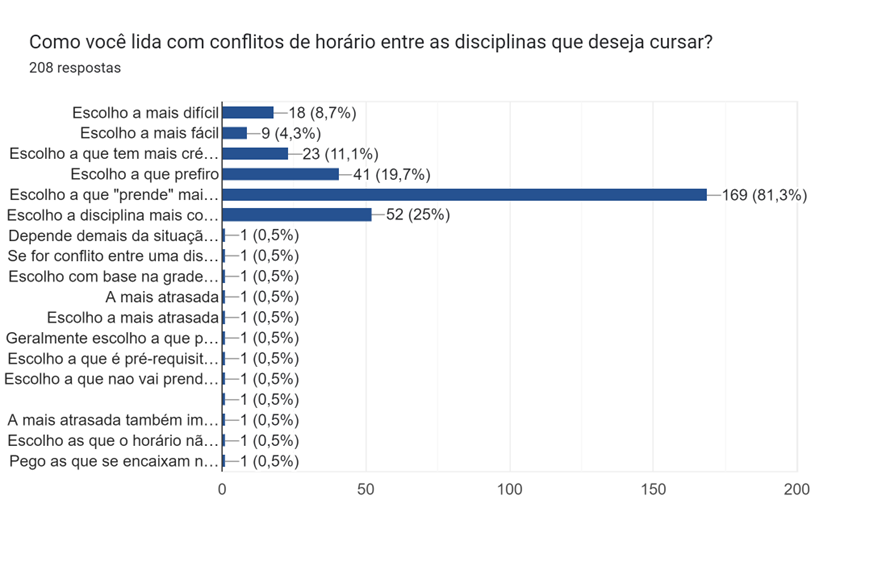
\includegraphics[scale=0.6]{files/img/Forms/4.3-PreferenciasPessoais-Conflitos.png}
  \legend{Fonte: o autor}
\end{figure} % PreferenciasPessoais Conflitos

Vale ressaltar que as respostas ilustradas pela Figura \ref{fig:4.3-PreferenciasPessoais-Conflitos} permite a seleção de múltiplas escolhas, inclusive permitindo que adicionassem outros critérios próprios. Dentre eles, um se mostrou ligeiramente recorrente que seria escolher a disciplina mais atrasada segundo a grade curricular. Outra possibilidade citada foi selecionar a que se encaixam na disponibilidade de horário pessoal, para que não conflite, por exemplo, com o horário do estágio obrigatório.

\begin{table}[htbp]
  \centering
  \caption{\label{table:4.3-PreferenciasPessoais-Conflitos}Critérios para a escolha de disciplinas conflituosas}
  \begin{tabular}{| r l |}
    \hline
    \textbf{Quantidade} & \textbf{Forma de escolher disciplina conflituosa} \\
    \hline
    169                 & Escolho a que "prende" mais matérias              \\
    52                  & Escolho a disciplina mais concorrida              \\
    41                  & Escolho a que prefiro                             \\
    23                  & Escolho a que tem mais créditos                   \\
    18                  & Escolho a mais difícil                            \\
    11                  & Outro                                             \\
    9                   & Escolho a mais fácil                              \\
    \hline
  \end{tabular}
\end{table}

\subsection{Experiências com atrasos e disciplinas} % #### 4.4.4. Experiências passadas com atrasos e disciplinas

Quanto aos atrasos para a realização de disciplinas, o ideal desejado é que não haja nenhum atraso. Nessa situação, todos os alunos que entram na universidade poderão seguir a disponibilidade usual das disciplinas dispostas em suas grades curriculares, que apresentam o período esperado para que cada disciplina seja realizada. Sendo elas, usualmente dividas como disciplinas pares e ímpares. As ímpares se referem às disciplinas em que se espera que sejam cursadas nos períodos 1, 3, 5, 7 e 9, e que são ofertadas no primeiro semestre letivo. Enquanto que as pares se referem às disciplinas oferecidas no segundo período letivo, onde geralmente se alocam as disciplinas dos períodos 2, 4, 6, 8 e 10.

Entretanto, a realidade dos alunos é outra. Isso se dá por diversos motivos, seja por reprovação, por não conseguir se inscrever na disciplina desejada ou por simplesmente não ter interesse em cursar a disciplina naquele momento, como já ilustrado na Figura \ref{fig:3.0_Satisfacao}. Esta característica se confirma na percepção da frequência e distância que percebemos dos atrasos, representado pelas Figuras \ref{fig:5.1-Atrasos-Esperar} e \ref{fig:5.2-Atrasos-Distancia}.

\begin{figure}[htbp]\centering
  \caption{\label{fig:5.1-Atrasos-Esperar}Períodos de atraso por espera}
  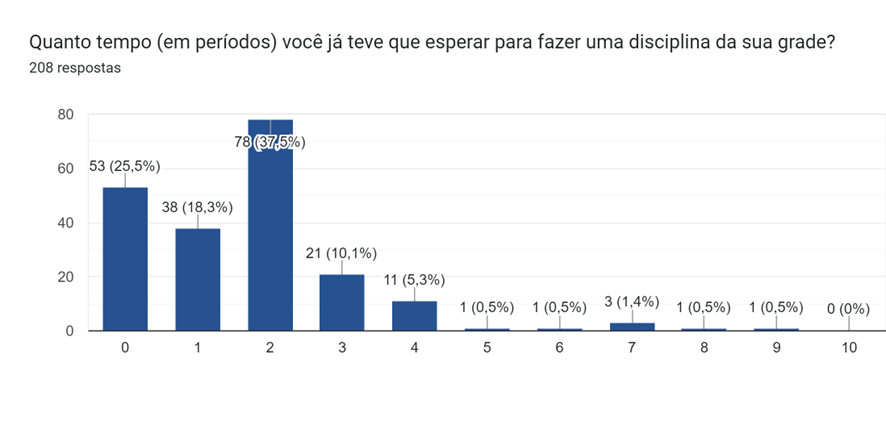
\includegraphics[scale=0.6]{files/img/Forms/5.1-Atrasos-Esperar.png}
  \legend{Fonte: o autor}
\end{figure} % Atrasos
\begin{figure}[htbp]\centering
  \caption{\label{fig:5.2-Atrasos-Distancia}Distância de atraso}
  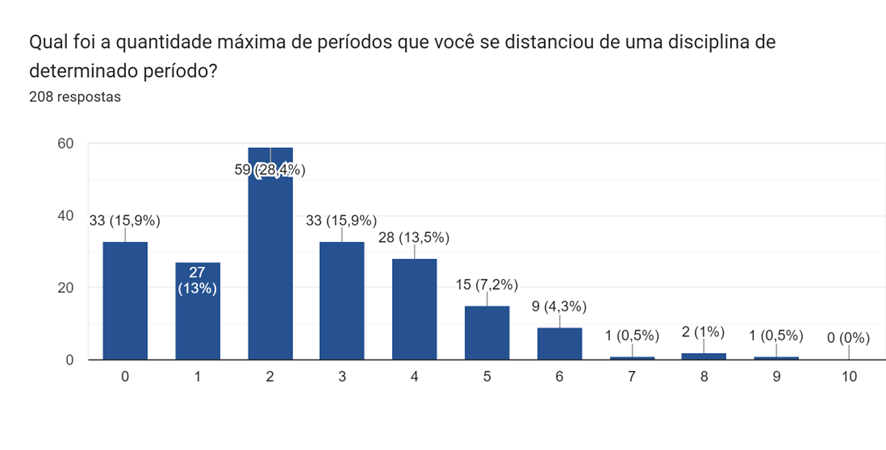
\includegraphics[scale=0.6]{files/img/Forms/5.2-Atrasos-Distancia.png}
  \legend{Fonte: o autor}
\end{figure} % Atrasos
Apresenta-se notável que é minoria a quantidade de alunos que nunca tiveram que esperar para cursar uma disciplina, sendo estes apenas 25,5\% dos respondentes. É ainda mais notável o fato de que o tempo de espera médio é de mais de um ano e meio. Quanto ao distanciamento de disciplinas, seja por reprovações ou por escolha própria se mostra ainda mais presente, sendo que apenas 15,9\% dos respondentes não se distanciaram das disciplinas esperadas para o período, sendo 2.8 anos o tempo médio de distanciamento.

Abaixo, encontra-se disposto na Tabela \ref{table:5.0-Atrasos} os resultados obtidos através desta seção do formulário.

\begin{enumerate}
  \item Quanto tempo (em períodos) você já teve que esperar para fazer uma disciplina da sua grade?
  \item Qual foi a quantidade máxima de períodos que você se distanciou de uma disciplina de determinado período?
\end{enumerate}


\begin{table}[htbp]
  \centering
  \caption{\label{table:5.0-Atrasos}Tempo de atraso em disciplinas}
  \begin{tabular}{| c | c c c c c c c c c c c |}
    \hline
    \multicolumn{1}{|c|}{\multirow{2}{*}{Pergunta}} &
    \multicolumn{11}{c|}{Períodos de atraso}                                                          \\
    \multicolumn{1}{|c|}{}                          &
    \multicolumn{1}{c|}{0}                          &
    \multicolumn{1}{c|}{1}                          &
    \multicolumn{1}{c|}{2}                          &
    \multicolumn{1}{c|}{3}                          &
    \multicolumn{1}{c|}{4}                          &
    \multicolumn{1}{c|}{5}                          &
    \multicolumn{1}{c|}{6}                          &
    \multicolumn{1}{c|}{7}                          &
    \multicolumn{1}{c|}{8}                          &
    \multicolumn{1}{c|}{9}                          &
    \multicolumn{1}{|c|}{10}
    \\
    \hline
    1                                               & 53 & 38 & 79 & 19 & 11 & 1  & 1 & 3 & 1 & 1 & 0 \\
    2                                               & 33 & 27 & 60 & 31 & 28 & 15 & 9 & 1 & 2 & 1 & 0 \\
    \hline
  \end{tabular}
\end{table}

\subsection{Pesquisa de opinião} % #### 4.4.5. Opiniões quanto à distribuição das disciplinas

Aqui, buscamos uma análise mais bruta e direta à concordância dos respondentes quanto às características atribuídas à distribuição de disciplinas semestrais, ondem eles avaliam com notas de 1 a 5 o quanto concordam com cada uma das características dadas à distribuição de disciplinas, sendo eles "Justa", "Variada", "Contínua", "Eficiente", "Distribuída" e "Satisfatória". Estando as opiniões dos alunos quanto às três primeiras refletidas nos resultados expostos pela Figura \ref{fig:6.0-Opiniao-1_3} enquanto que as três últimas são ilustradas pela Figura \ref{fig:6.0-Opiniao-4_6}.

% \begin{figure}[htbp]
%     \centering
%     \caption{\label{fig:6.0-Opiniao-Todas}Notas dadas para as características  da distribuição de disciplinas}
%     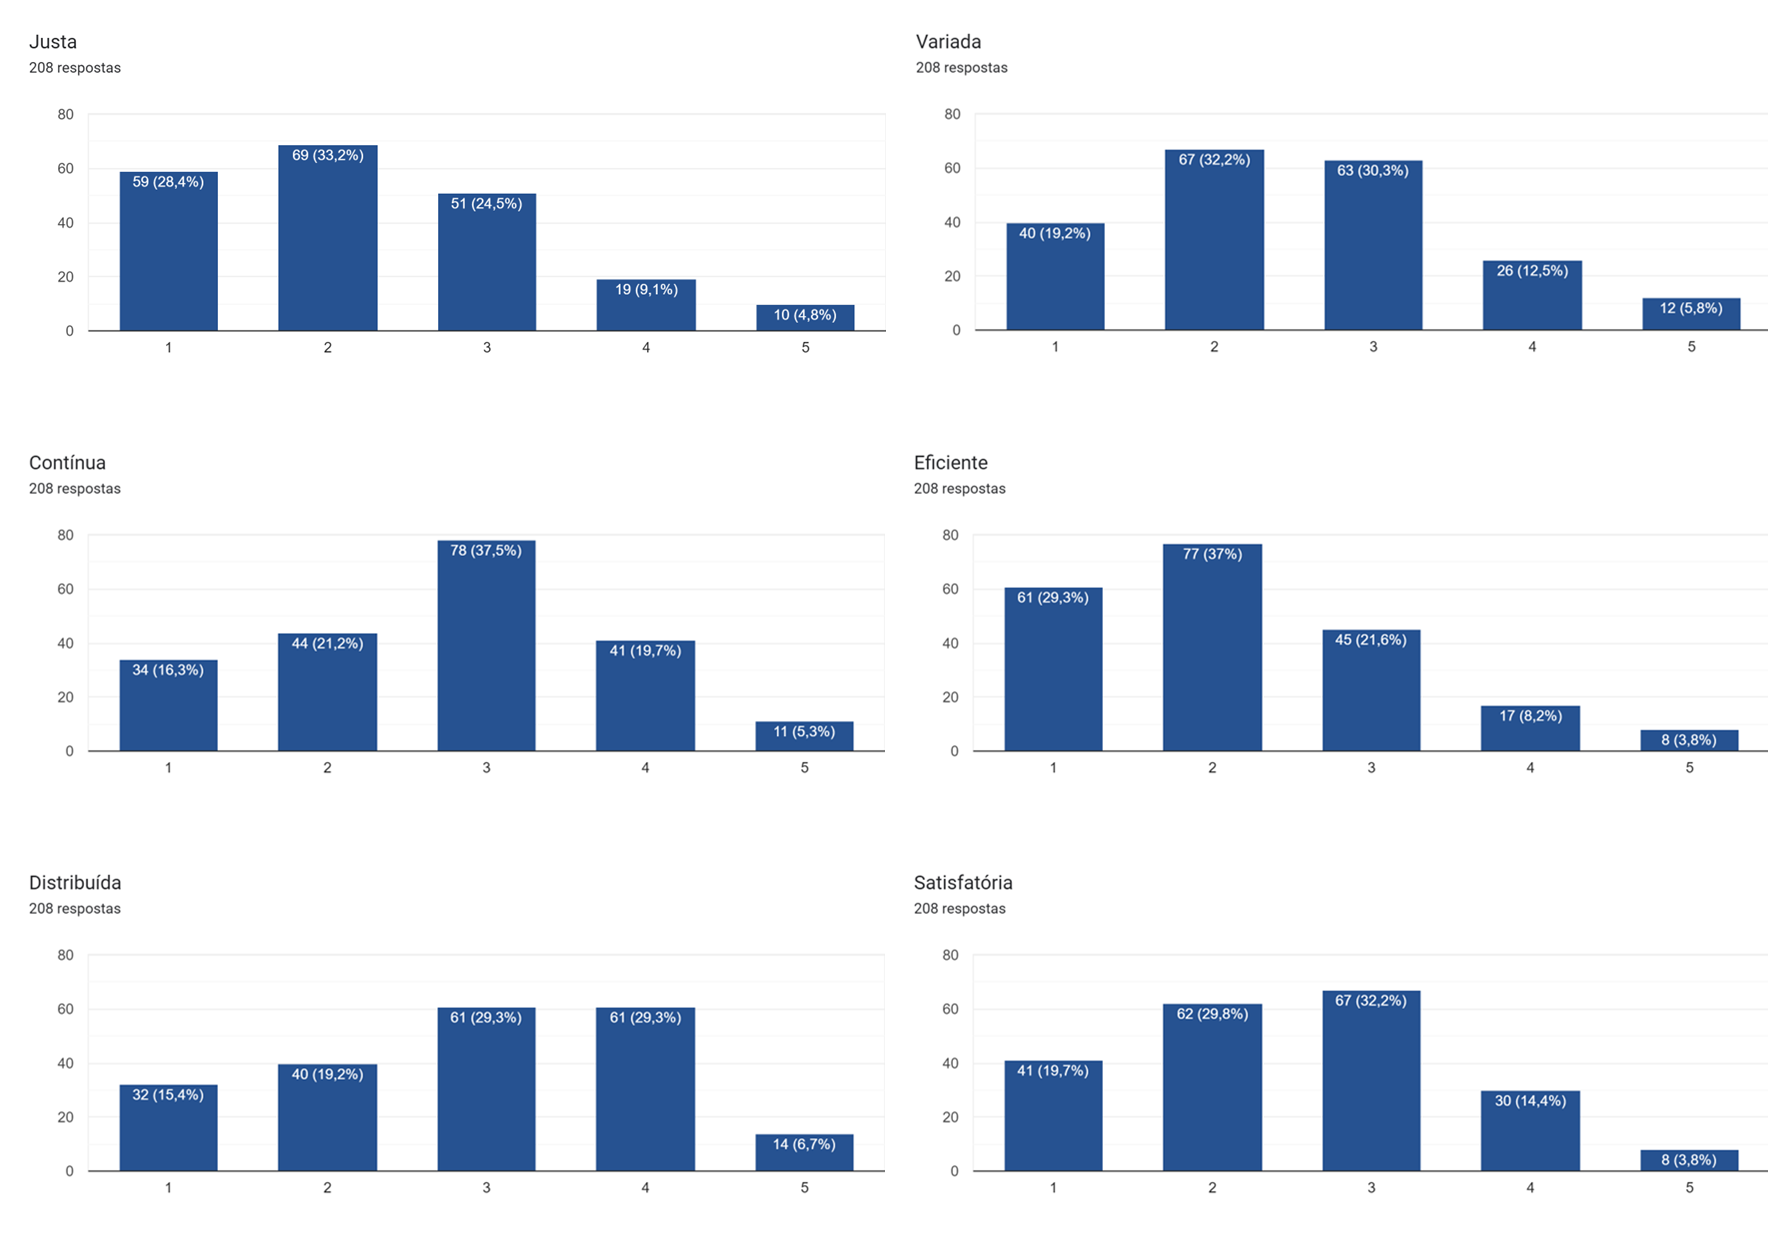
\includegraphics[scale=0.4]{files/img/Forms/6.0-Opiniao-Todas.png}
%     \legend{Fonte: o autor}
% \end{figure}

\begin{figure}[htbp]
  \centering
  \caption{\label{fig:6.0-Opiniao-1_3}Notas dadas para as características "Justa", "Variada" e "Contínua" da distribuição de disciplinas}
  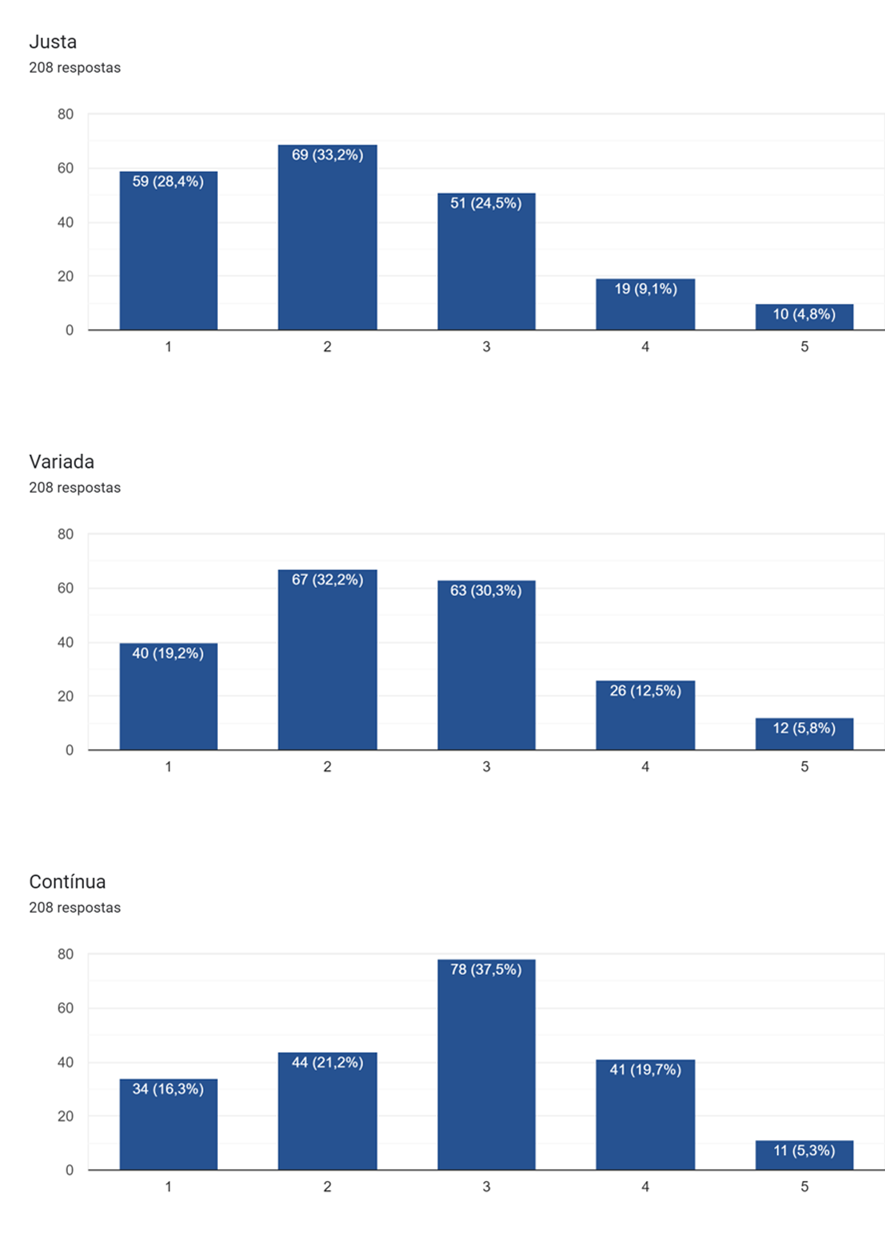
\includegraphics[scale=0.4]{files/img/Forms/6.0-Opiniao-1_3.png}
  \legend{Fonte: o autor}
\end{figure}

\begin{figure}[htbp]
  \centering
  \caption{\label{fig:6.0-Opiniao-4_6}Notas dadas para as características "Eficiente", "Distribuída" e "Satisfatória" da distribuição de disciplinas}
  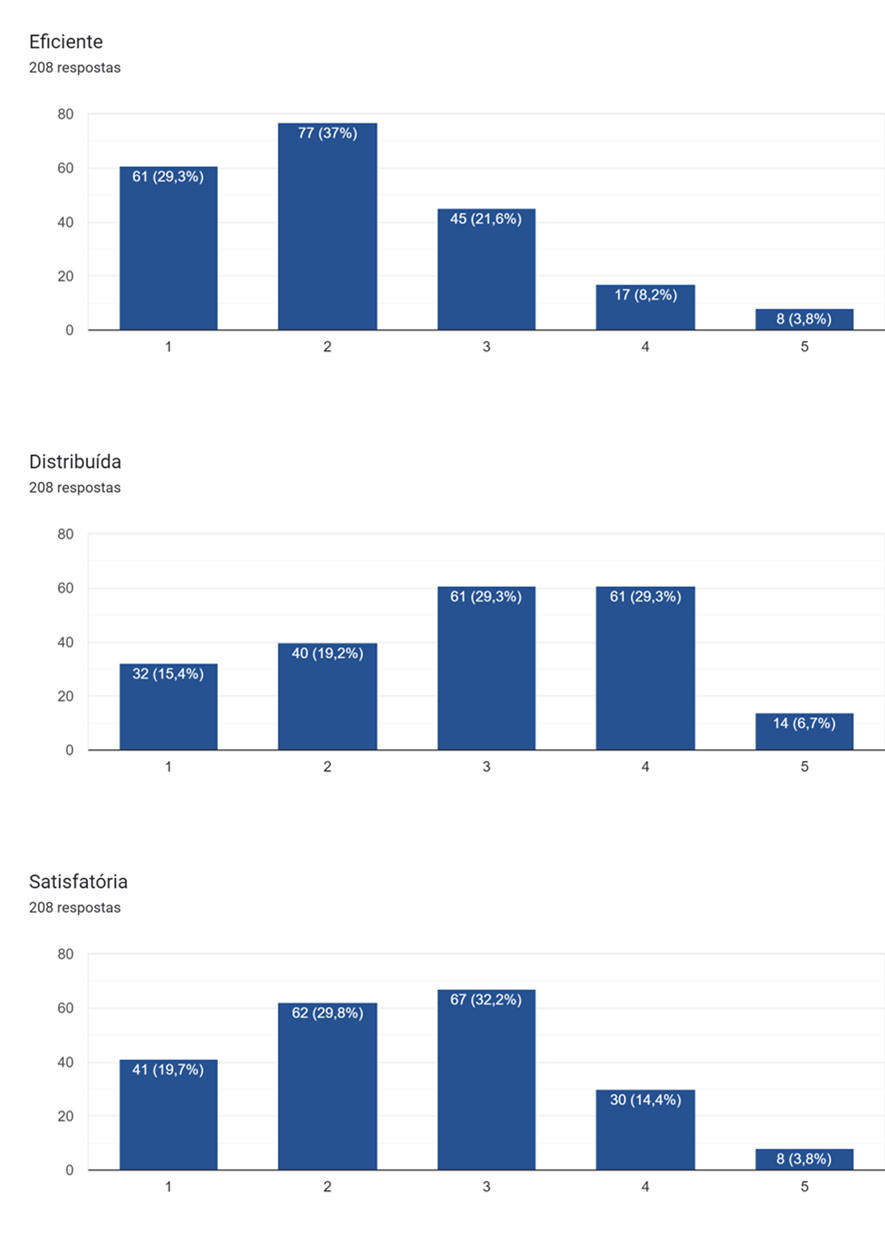
\includegraphics[scale=0.4]{files/img/Forms/6.0-Opiniao-4_6.png}
  \legend{Fonte: o autor}
\end{figure}

% \begin{figure}[htbp]\centering
%     \caption{\label{fig:6.1-Opiniao-Justa.png}Notas dadas para a característica: justa}
%     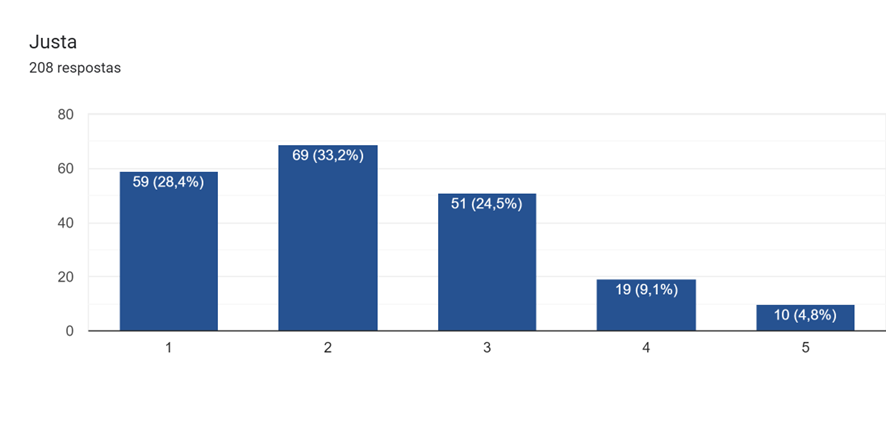
\includegraphics[scale=0.6]{files/img/Forms/6.1-Opiniao-Justa.png}
%     \legend{Fonte: o autor}
% \end{figure} % Opiniao-Justa

% \begin{figure}[htbp]\centering
%     \caption{\label{fig:6.2-Opiniao-Variada.png}Notas dadas para a característica: variada}
%     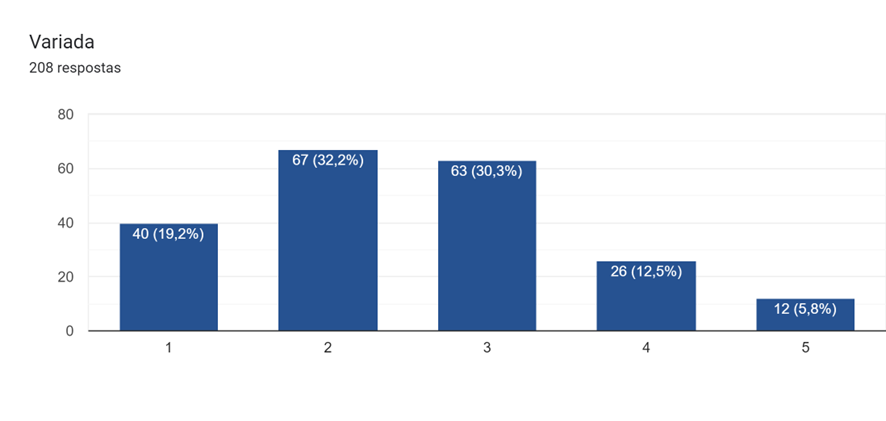
\includegraphics[scale=0.6]{files/img/Forms/6.2-Opiniao-Variada.png}
%     \legend{Fonte: o autor}
% \end{figure} % Opiniao-Variada

% \begin{figure}[htbp]\centering
%     \caption{\label{fig:6.3-Opiniao-Continua.png}Notas dadas para a característica: contínua}
%     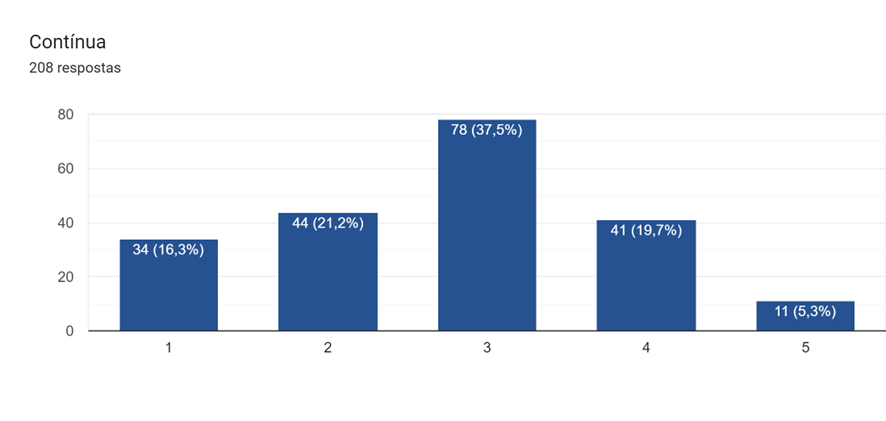
\includegraphics[scale=0.6]{files/img/Forms/6.3-Opiniao-Continua.png}
%     \legend{Fonte: o autor}
% \end{figure} % Opiniao-Continua

% \begin{figure}[htbp]\centering
%     \caption{\label{fig:6.4-Opiniao-Eficiente.png}Notas dadas para a característica: eficiente}
%     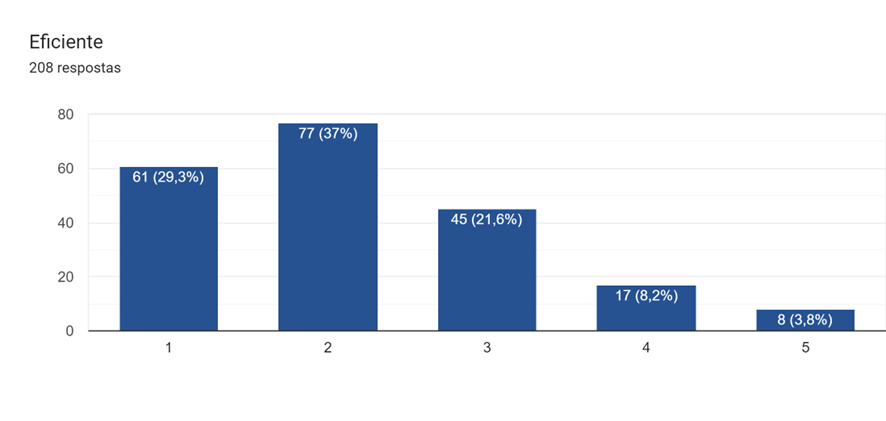
\includegraphics[scale=0.6]{files/img/Forms/6.4-Opiniao-Eficiente.png}
%     \legend{Fonte: o autor}
% \end{figure} % Opiniao-Eficiente

% \begin{figure}[htbp]\centering
%     \caption{\label{fig:6.5-Opiniao-Distribuida.png}Notas dadas para a característica: distribuída}
%     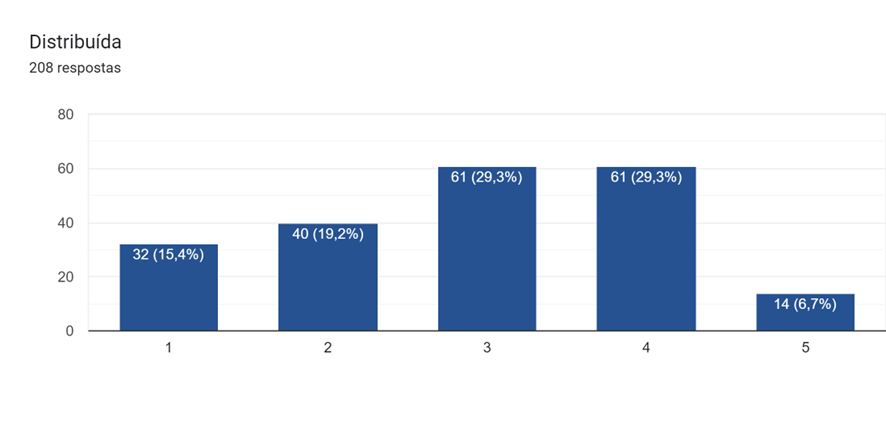
\includegraphics[scale=0.6]{files/img/Forms/6.5-Opiniao-Distribuida.png}
%     \legend{Fonte: o autor}
% \end{figure} % Opiniao-Distribuida

% \begin{figure}[htbp]\centering
%     \caption{\label{fig:6.6-Opiniao-Satisfatoria.png}Notas dadas para a característica: satisfatória}
%     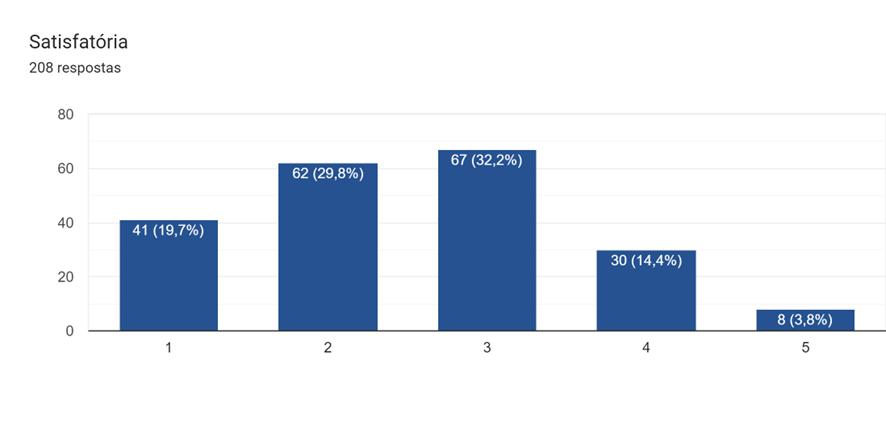
\includegraphics[scale=0.6]{files/img/Forms/6.6-Opiniao-Satisfatoria.png}
%     \legend{Fonte: o autor}
% \end{figure} % Opiniao-Satisfatoria

De uma forma geral, conseguimos ver todos os gráficos com menos de 7\% dos respondentes dando nota 5 em cada uma das características, A maioria das respostas tende a estar entre 1 e 3, sendo exceção apenas no caso da característica "distribuída", que por sua vez apresenta uma elevada quantidade de notas 4, sendo referente a 29,3\% dos respondentes.

Como forma tabular, temos, na Tabela \ref{table:6.0-Opiniao}, as respostas dos alunos, seguidas das médias por característica.

\begin{table}[htbp]
  \centering
  \caption{\label{table:6.0-Opiniao}Notas dadas às características da distribuição de disciplinas}
  \begin{tabular}{| l | c c c c c | c |}
    \hline
    \multicolumn{1}{|c|}{\multirow{2}{*}{Opções}} &
    \multicolumn{5}{c|}{Notas}                    &
    \multicolumn{1}{|c|}{\multirow{2}{*}{Médias}}
    \\
    \multicolumn{1}{|c|}{}                        &
    \multicolumn{1}{c|}{1}                        &
    \multicolumn{1}{c|}{2}                        &
    \multicolumn{1}{c|}{3}                        &
    \multicolumn{1}{c|}{4}                        &
    \multicolumn{1}{c|}{5}                        &
    \multicolumn{1}{|c|}{}                                                       \\
    \hline
    Justa                                         & 59 & 69 & 52 & 17 & 10 & 2,3 \\
    Variada                                       & 40 & 65 & 64 & 26 & 12 & 2,5 \\
    Contínua                                      & 34 & 44 & 78 & 41 & 10 & 2,8 \\
    Eficiente                                     & 61 & 76 & 45 & 17 & 8  & 2,2 \\
    Distribuída                                   & 32 & 40 & 61 & 60 & 14 & 2,9 \\
    Satisfatória                                  & 40 & 61 & 68 & 30 & 8  & 2,5 \\
    \hline
  \end{tabular}
\end{table}

Ao analisarmos a média de cada uma, podemos dizer que, em suma, há o visível desagrado do corpo discente quanto à distribuição de disciplinas semestrais, com ênfase nas duas piores notas que são 2,2 para "eficiente" e 2,3 para "justa" o que reforça a necessidade de aprimoramento do sistema atual.

\subsection{Respostas qualitativas} % #### 4.4.6. Respostas qualitativas

Por fim, havia um espaço livre no formulário para que os alunos pudessem expressar suas opiniões de forma mais livre. Após a leitura de todas e a filtragem das opiniões expressas, resumem-se em 4 parabenizações pelo desenvolvimento do presente projeto, 18 reclamações e 16 sugestões. Dentre elas, algumas apresentaram maior recorrência, sendo elas:

\begin{itemize}
  \item 5 reclamações sobre a usual oferta de disciplinas separadas entre pares e ímpares;
  \item 4 reclamações sobre o Sistema Acadêmico, principalmente sobre não ser capaz de suportar a carga nos momentos iniciais de inscrição de disciplinas;
  \item 3 sugestões de ofertas de disciplinas recorrentemente, com ênfase nas disciplinas de matemática/que contemplam diversos cursos/com alta taxa de reprovação;
  \item 3 sugestões de mais oferta de disciplinas no período de verão;
  \item 2 sugestões de que inscrições em matérias do semestre atual esperado do aluno fossem feitas automaticamente, mas ainda permitindo a sua exclusão caso desejado;
  \item 1 sugestão de criação de um formulário de demanda no acadêmico que computasse a intenção de matrícula dos alunos.
\end{itemize}

Abaixo estão dispostas algumas das respostas obtidas:

\begin{itemize}
  \item "A estrutura curricular deveria ser predefinida, automatizando a matrícula dos alunos nas disciplinas correspondentes aos seus períodos acadêmicos. No entanto, permitir-se-ia a edição do cronograma por parte dos alunos, caso desejem quitar pendências de períodos anteriores ou disciplinas antecipadas. Além disso, disciplinas que abrangem múltiplos cursos devem ser oferecidas em ambos os semestres.

        Para melhorar a oferta de disciplinas, seria aconselhável ampliar a disponibilidade de disciplinas durante o período de verão. Isso facilitaria o acesso dos alunos ao estágio obrigatório durante as férias, viabilizando a conclusão dessa etapa essencial do curso. Reduzir o número de créditos necessários para antecipar a realização do estágio também se mostraria benéfico, visto que atualmente, a conclusão dessa matéria com apenas 9 créditos pendentes inviabiliza a possibilidade de antecipação antes do 9º período. Considera-se viável permitir essa antecipação a partir do 7º período.

        [...]
        Essas melhorias no sistema acadêmico [...] agilizariam a trajetória do estudante, permitindo maior flexibilidade na escolha e realização de disciplinas [...]."
  \item "Existe muita desorganização em relação a grade, disciplinas e sistema acadêmico por parte dos coordenadores dos cursos. Me inscrevi numa matéria que tinha requisito de acordo com o plano pedagógico, mas tanto na grade como no sistema acadêmico não tinha pré-requisito nenhum. Tive que desistir da matéria pela dificuldade, até porque a matéria que era pré-requisito eu perdi. Detalhe: Outras pessoas perderam na matéria pré-requisito e continuaram fazendo a matéria desse período."
  \item "Acho que as coordenações precisam estabelecer um melhor diálogo com os alunos. Esse sistema de período par e Ímpar na UENF é antigo e perpetua um comodismo dos professores que acabam não ofertando disciplinas todos os semestres e prejudicando os alunos nas escolhas de matérias optativas, eletivas, instrumentais e obrigatórias tendo que esperar um ano para realizar a disciplina caso você não consiga fazer por choque de horário e/ou reprovação."
\end{itemize}

\subsection{Conclusões} % #### 4.4.7. Conclusões

Por fim, entendemos que, além das insatisfações dormentes por parte dos gestores e criadores de grades horárias, os alunos também se mostram insatisfeitos com a atual estrutura de distribuição de disciplinas semestrais. Os interesses dos alunos se mostram em sua maioria alinhados com os interesses dos gestores, onde ambos visam reduzir a quantidade de atrasos na progressão do curso.

\section{Exemplo de erros humanos} % contém as imagens que estavan o cap 1


Dada a grande quantidade de variáveis interconectadas e as características específicas de cada instituição \cite{miranda_udpskeduler_2012}, a organização destas informações buscando a melhor solução possível apresenta-se como um desafio. Principalmente se considerarmos que esta solução é, muitas vezes, buscada manualmente, estando também passível de erros humanos como ilustram as Figuras \ref{Academico} e \ref{CCT}.

% ![Disciplina atribuída no sistema acadêmico à determinada hora e local](img/Falha_de_alocacao/Metodologia-Quinta.png)

% ![Disciplina não atribuída à determinada hora e local na grade de horários do CCT](img/Falha_de_alocacao/Aulas-CCT-105-2023_1.png)

\begin{figure}[htbp]\centering
  \caption{\label{Academico}Disciplina atribuída no sistema acadêmico à determinada hora e local}
  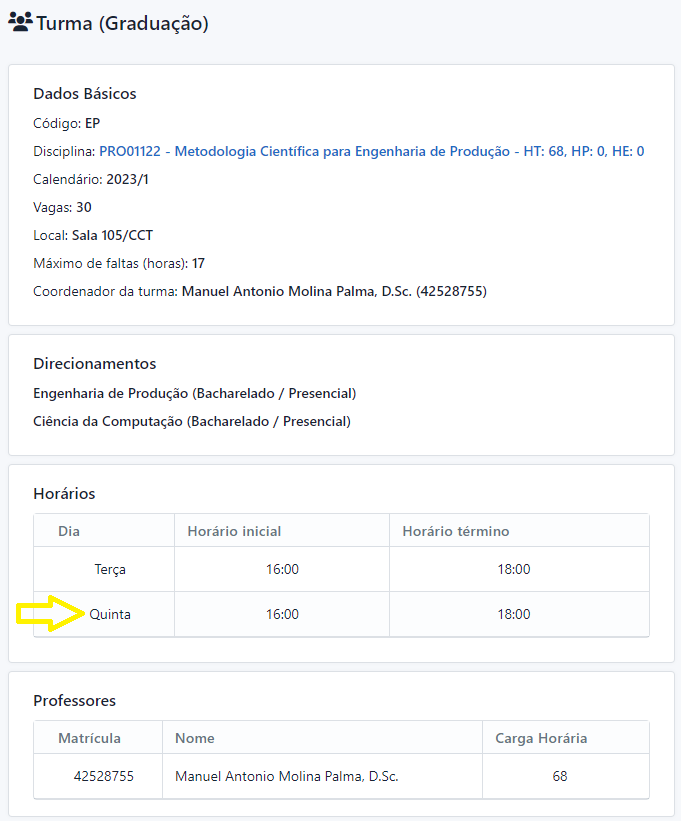
\includegraphics[angle=0,scale=0.8]{files/img/FalhaDeAlocacao/Metodologia-Quinta.png}
  \legend{Fonte: o autor}
\end{figure}    % Imagem acadêmico

\begin{figure}[htbp]\centering
  \caption{\label{CCT}Disciplina não atribuída à determinada hora e local na grade de horários do CCT}
  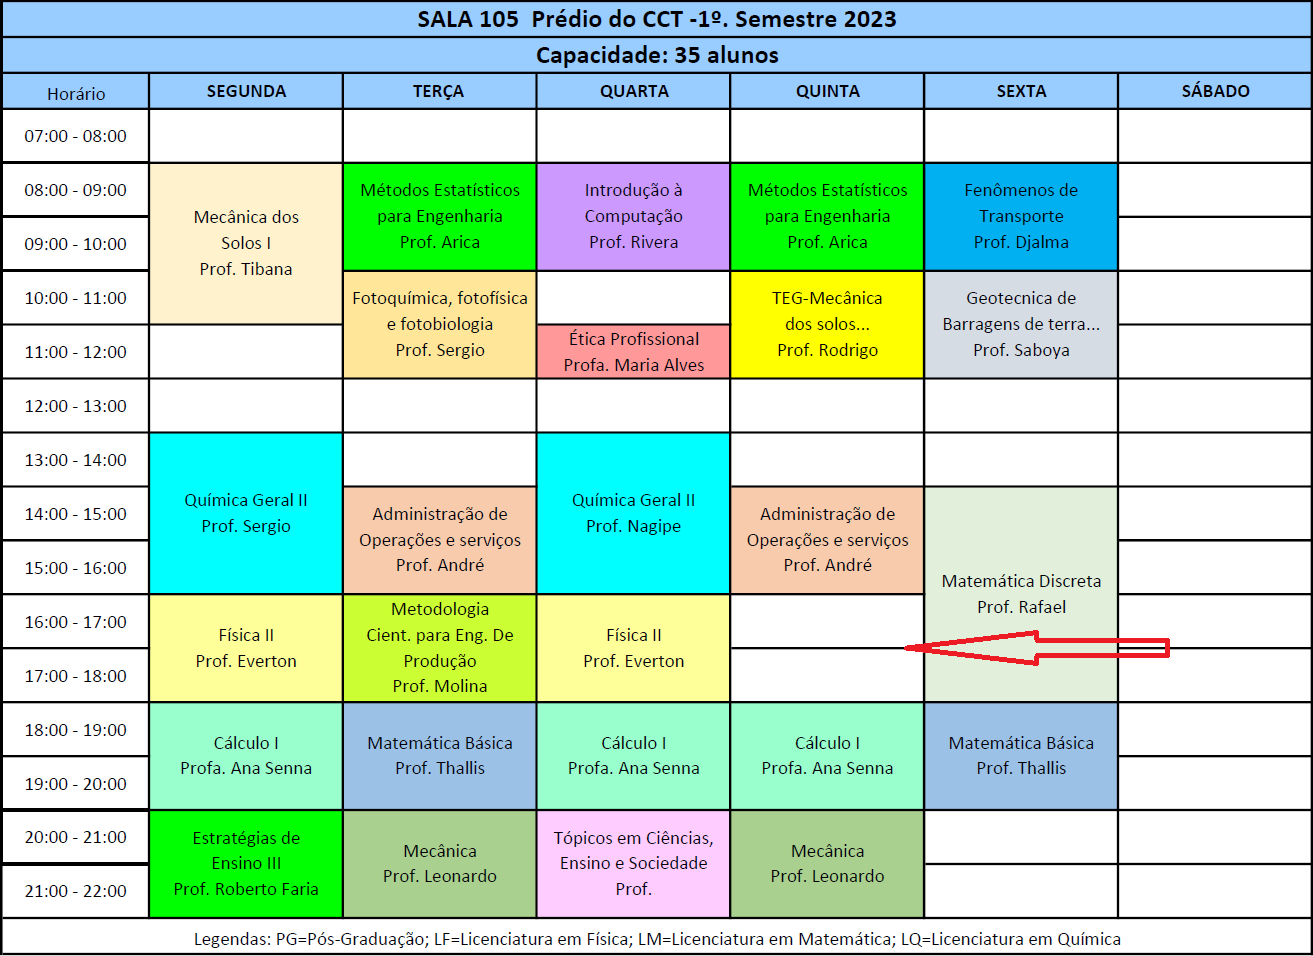
\includegraphics[angle=0,scale=0.5]{files/img/FalhaDeAlocacao/Aulas-CCT-105-2023_1.png}
  \legend{Fonte: o autor}
\end{figure}    % Imagem representando o erro humano na alocação de salas

Nestas imagens, fica exemplificado um dos possíveis problemas que podem ocorrer durante a criação de grades horárias, que é, mesmo quando uma seção da universidade (o Sistema Acadêmico, ilustrado pela Figura \ref{Academico}) aloca uma turma a uma determinada sala, outra seção da mesma instituição (o Centro de Ciência e Tecnologia, ilustrado pela Figura \ref{CCT}) pode não estar ciente do mesmo, ou mesmo estando ciente pode acabar não delimitando aquela lacuna de tempo como ocupada, assim estando passível de uma segunda alocação naquele período de tempo naquela sala, assim gerando problemas.
% \chapter{Modelagem geral do sistema} \label{chap:modelagem}

Tendo esclarecido sobre as questões gerais do trabalho e da área de estudo. Agora nos aprofundaremos um pouco mais na modelagem e criação de diagramas que ilustrem o funcionamento geral do sistema e a forma como se dará a execução da metodologia proposta.

\section{Estágios de execução}

Em seu trabalho de aplicação prática, \cite{miranda_udpskeduler_2012} estruturou estágios que compõem o processo necessário para que enfim se alcance a definição de \textit{timetables} ótimas.

\begin{figure}[htbp]\centering
  \caption{Estágios para a obtenção de grade horária ótima}
  \label{fig:geral}
  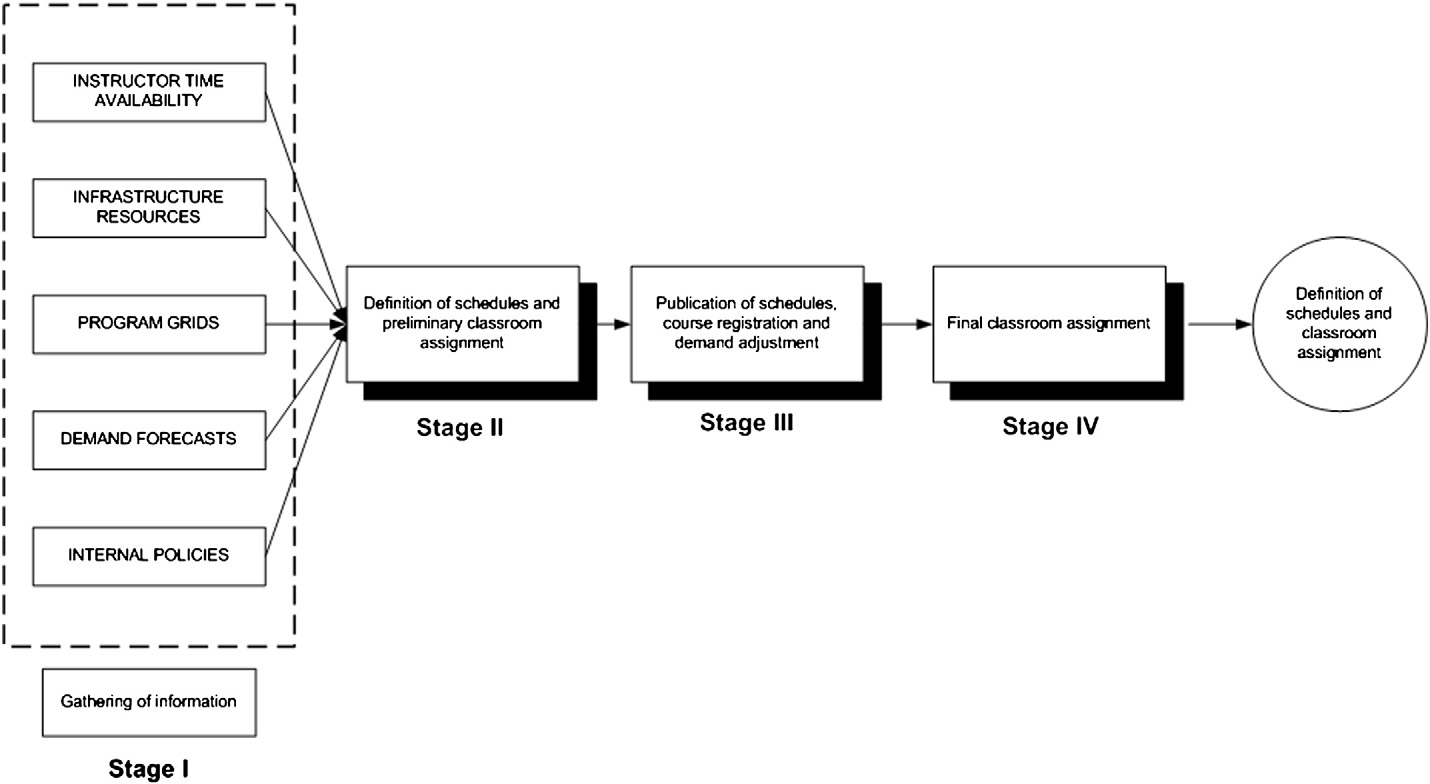
\includegraphics[width=\textwidth]{files/img/Arquitetura/Arquitetura-UDP}
  \legend{Fonte: \cite{miranda_udpskeduler_2012}}
\end{figure}

Na \autoref{fig:geral}, estão dispostos 4 estágios principais. O primeiro dispõe da aquisição de informações. O meio de aquisição não é relevante para o momento atual, apenas considera-se que esta informação será obtida. No segundo estágios são definidas grades horárias preliminares para se atribuir os alunos. No terceiro, os alunos se inscrevem e a demanda é ajustada, por fim, no quarto estágio, ocorre a alocação final das salas.

\section{Iteração}

Para se alcançar uma alta satisfação por parte dos \textit{stakeholders}, vê-se necessária a constante interação com os mesmos. Para isto, será seguida a estrutura utilizada por \cite{andre_interaction_2018}.

\begin{figure}[htbp]\centering
  \caption{Etapas do Design de Interação}
  \label{fig:IxD}
  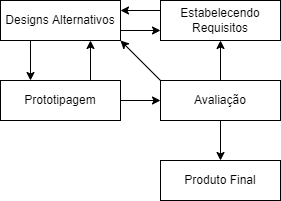
\includegraphics{files/img/Arquitetura/Arquitetura-IxD}
  \legend{\selfAuthor}
\end{figure}    % University

Seguindo o conceito do Design de Interação, a \autoref{fig:IxD} ilustra o ciclo de ações a serem tomadas durante o desenvolvimento do sistema, caso este venha a ser necessário. Neste modelo de pesquisa, os \textit{stakeholders} serão consultados continuamente enquanto lhes é apresentado protótipos do sistema, para que assim informem quanto às suas percepções. Esta dinâmica tem como finalidade encontrar um design tal que seja adequado aos desejos e necessidades de seus usuários finais.

\section{Funcionamento}

O sistema final seguirá uma dinâmica similar à que foi ilustrada por \cite{bebis_information_2019} em seu trabalho sobre o uso da Visualização de Informações em relação às Ed-TTPs.

\begin{figure}[htbp]\centering
  \caption{Funcionamento geral do sistema}
  \label{fig:sistema}
  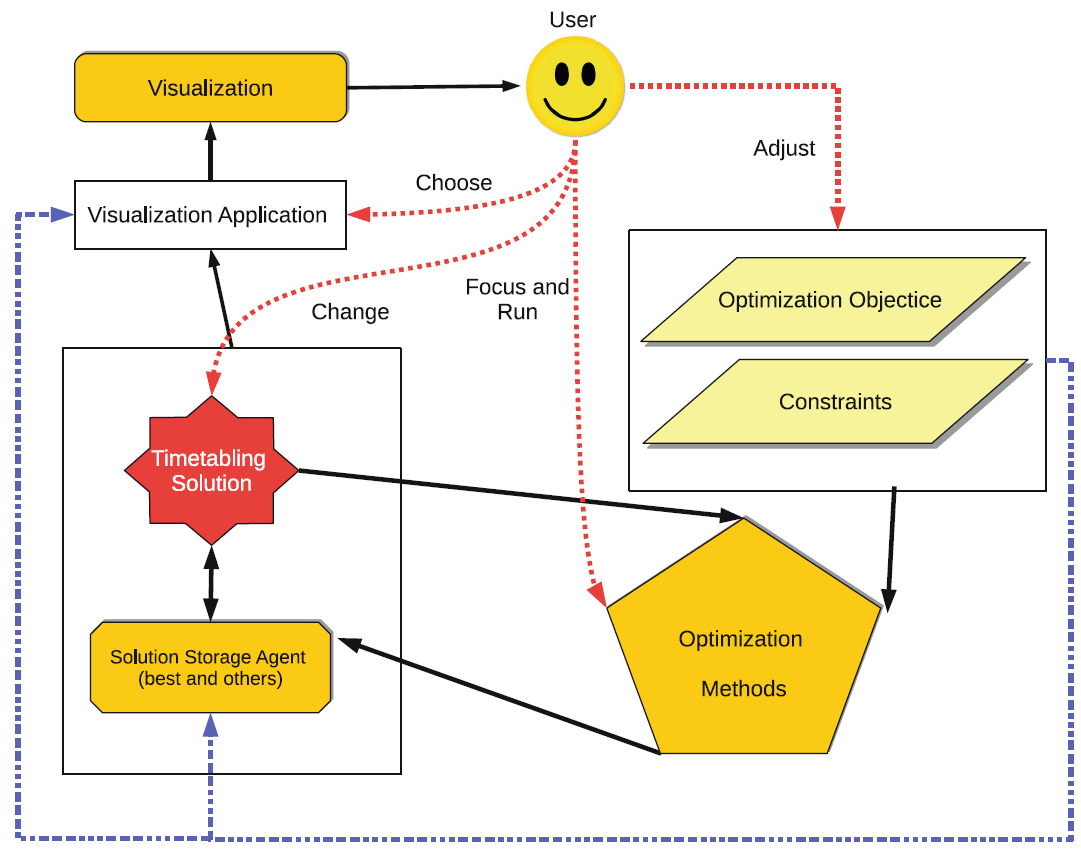
\includegraphics[width=\textwidth]{files/img/Arquitetura/Arquitetura_bebis_information_2019}
  \legend{Fonte: \cite{bebis_information_2019}}
\end{figure}

A \autoref{fig:sistema} apresenta o comportamento geral do sistema, como seus diferentes segmentos interagem entre si e de que forma o usuário interage com o mesmo. O usuário poderá ajustar os objetivos da otimização e suas restrições, elas serão utilizadas nos métodos de otimização. Estes métodos serão utilizados para se alcançar soluções para estes critérios, as melhores serão então armazenadas. Em posso destes dados, a aplicação apresentará visualmente estas informações ao usuário, permitindo que ele interaja dinamicamente a fim de alcançar seus objetivos.

\section{Modelo de Banco de Dados} \label{sec:ModelagemBD} % ### 5.4. Modelo de Banco de Dados

Considerando as informações necessárias para o presente trabalho, e também o preparo de campo para potenciais aplicações futuras, foi elaborado um diagrama conceitual de banco de dados, que pode ser visto na \autoref{fig:DiagramConceitual}.

\begin{MyCenteredFigure}
  \caption{Diagrama Conceitual do banco de dados}
  \label{fig:DiagramConceitual}
  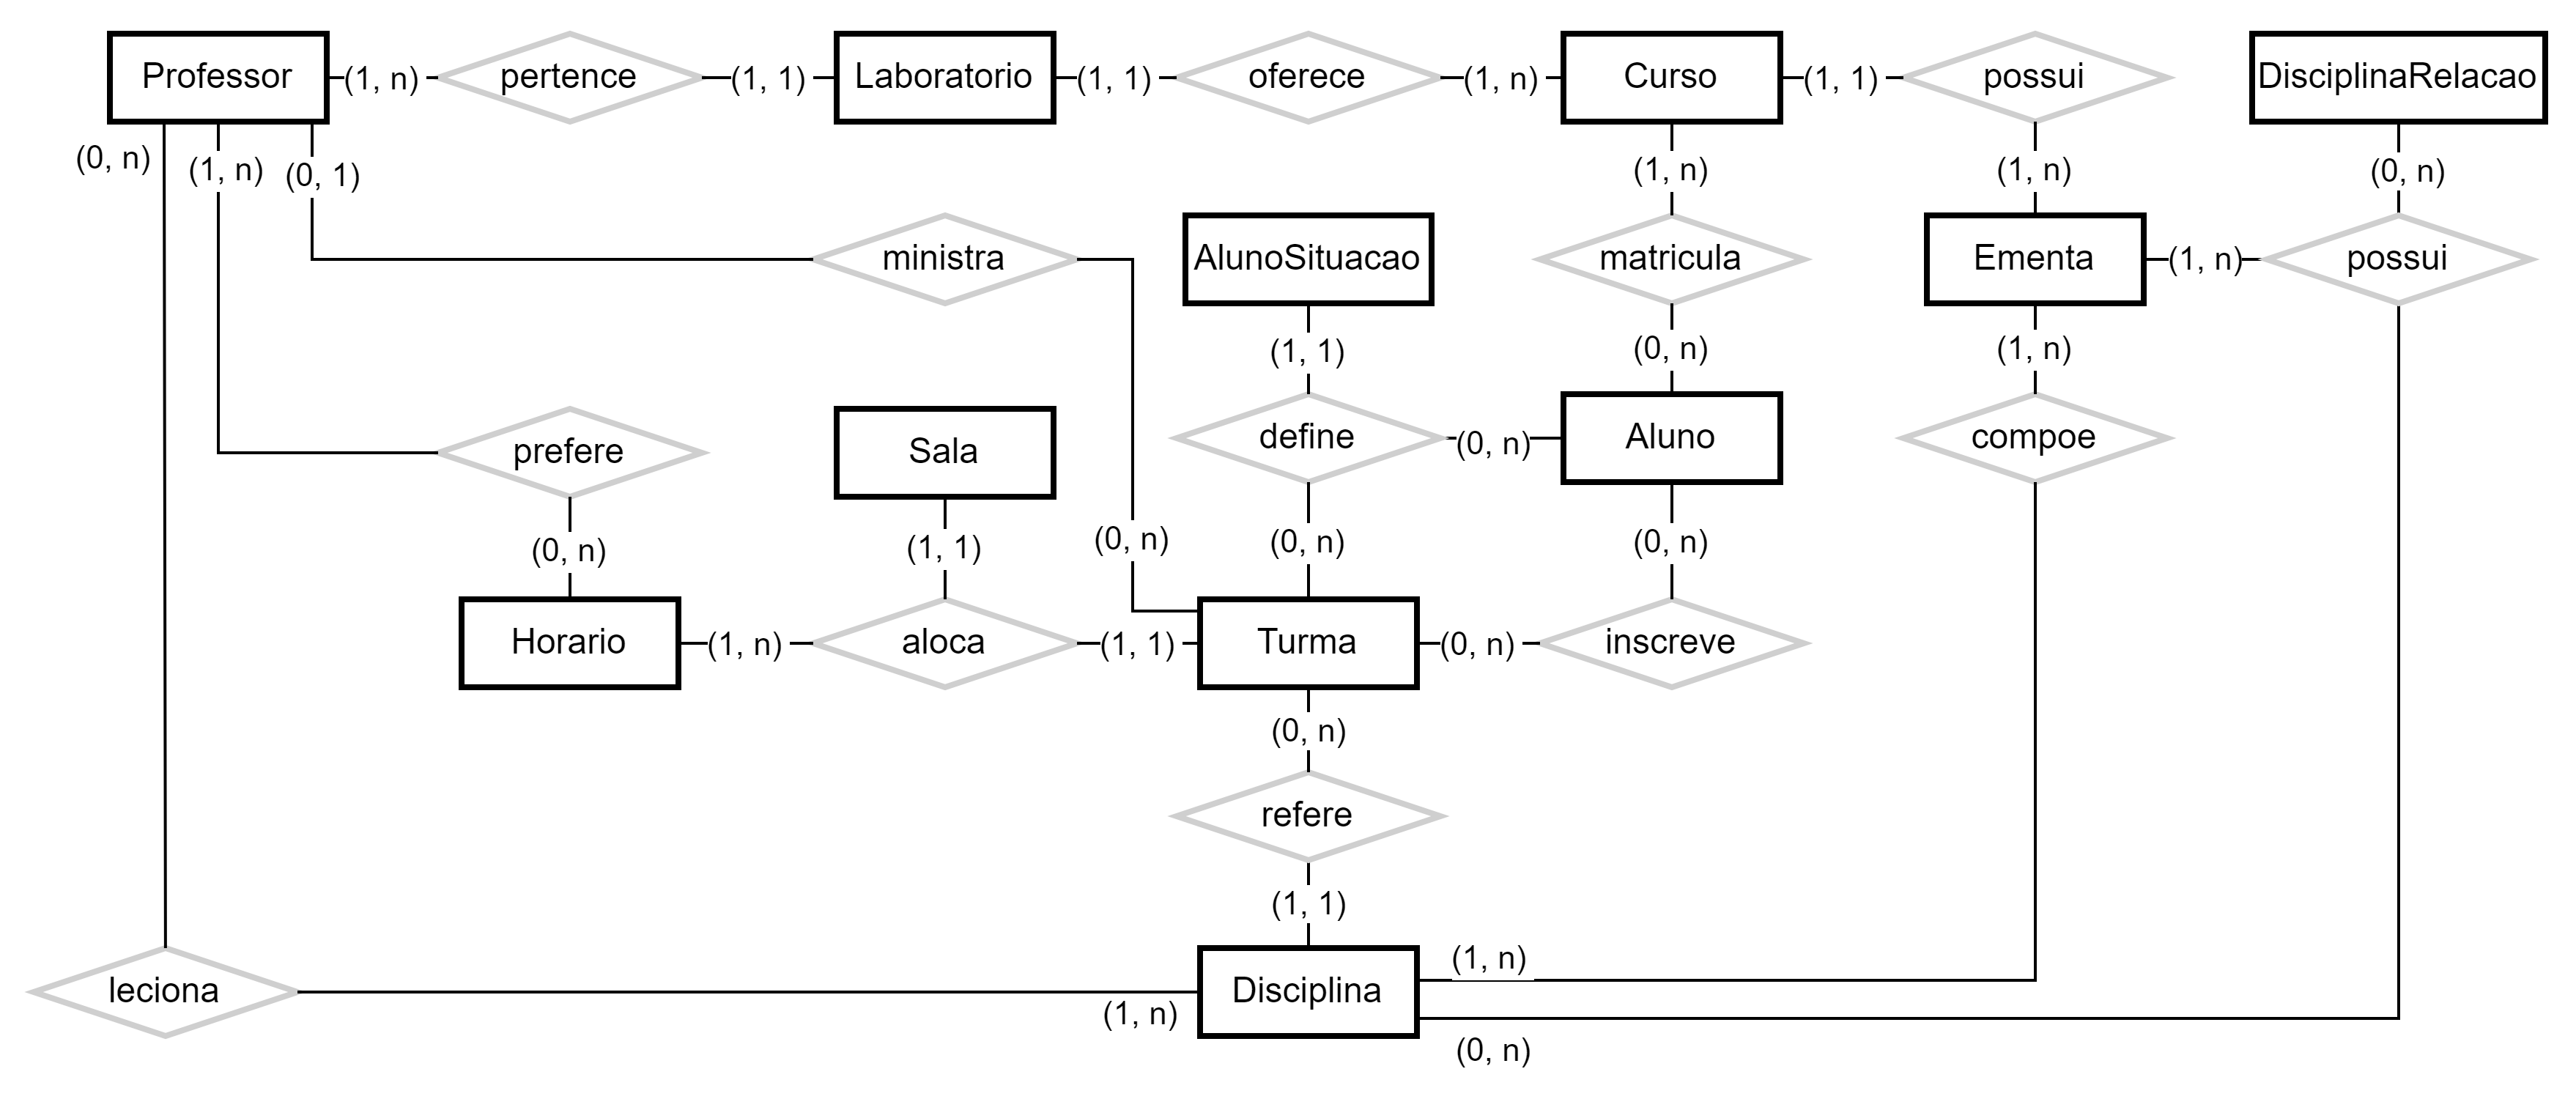
\includegraphics[width=\textwidth]{files/img/DiagramaConceitual/DiagramaConceitualBranco}
\end{MyCenteredFigure} % Diagrama Conceitual

O diagrama conceitual foi elaborado utilizando a ferramenta \href{https://www.drawio.com/}{draw.io} citada na metodologia e ilustra as relações entre diversas entidades presentes na realidade da UENF. O emaranhamento presente no diagrama ilustra a complexidade envolvida na criação de uma grade horária, onde diversas entidades se relacionam entre si.

Como principais apontamentos, podemos citar a parte principal do modelo que é a alocação de turmas. Ela, como já descrito, envolve a correlação entre alunos de diferentes cursos, professores, disciplinas, salas e horários. Além disso, também é possível notar a presença de entidades que não são diretamente relacionadas à alocação de turmas, mas que podem se mostrar úteis, como a relação entre professores e laboratórios, e a de disciplinas e ementas.

Embora o diagrama apresente uma visão mais completa de todas as interconexões possíveis, é importante ressaltar que o presente trabalho foca primordialmente na alocação das turmas para o curso de Ciência da Computação, e que a implementação do banco de dados será feita de forma a atender a essas necessidades, fazendo então uso de uma parte do diagrama conceitual.

% Tendo isso em vista, o modelo conceitual reduzido para o presente trabalho pode ser visto na \autoref{fig:DiagramConceitualReduzido}.

% \begin{MyCenteredFigure}
%  \caption{Diagrama Conceitual reduzido para o presente trabalho}
%  \label{fig:DiagramConceitualReduzido}
%  \includegraphics[width=\textwidth]{files/img/DiagramaConceitual/DiagramaConceitualReduzidoBranco}
% \end{MyCenteredFigure} % Diagrama Conceitual reduzido

Neste modelo, mais enxuto, temos apenas as entidades principais, onde temos uma turma de determinada disciplina, ministrada por um professor e que ocorre em uma sala em um determinado horário.

\subsection{Diagrama de Entidade e relacionamento} % ### 5.4.1. Modelo Relacional

% Com isso, restamos o diagrama de Entidade e Relacionamento (DER) que pode ser visto na \autoref{fig:DER}.

% \begin{MyCenteredFigure}
%  \caption{Diagrama de Entidade e Relacionamento}
%  \label{fig:DER}
%  \includegraphics[width=\textwidth]{files/img/DER/DERBranco}
% \end{MyCenteredFigure} % Diagrama de Entidade e Relacionamento

Neste diagrama vemos as entidades principais, que são \textit{Turmas}, \textit{Disciplinas}, \textit{Professores}, \textit{Horários} e \textit{Salas}. As propriedades escolhidas para cada entidade são compostas por uma mistura de critérios. Por exemplo, o nome do professor, o código da disciplina, e a junção de código e bloco auxiliam primordialmente na identificação real dos professores, disciplinas e salas. Já as informações ``período'', ``apelido'' e ``comment''...

E também é notável a presença da entidade \textit{Alunos}, que se apresenta desacoplado das demais entidades. O motivo para isso é que, embora os alunos façam parte do processo de alocação de turmas, ao longo do desenvolvimento, o desenvolvimento de funcionalidades envolvendo os alunos...

% \chapter{Desenvolvimento} \label{chap:desenvolvimento}

% Citar alguns códigos

Para o desenvolvimento do presente trabalho, foram utilizadas diversas ferramentas, tanto para a elaboração do código, quanto para a elaboração do modelo de banco de dados e para a elaboração do protótipo. Todas elas com o intuito de implementar o software necessário para a criação de uma grade horária.

\section{Projetos anteriores} % ### 5.1. Pré desenvolvimento

Antes do desenvolvimento do presente trabalho, foram feitos alguns projetos pessoais que, embora não tenham sido concluídos, serviram como base para o desenvolvimento do presente trabalho.

\subsection{Andamento dos alunos} % #### 5.1.1. Andamento dos alunos

Como interesse próprio, cogitou-se o desenvolvimento de uma plataforma onde se pudesse ver em que ponto os alunos se encontram em relação ao andamento de seus cursos. Para isso, seria necessária a obtenção dos dados dos alunos, seja por parte dos mesmos, do coordenador ou por integração com o sistema acadêmico. Com estes dados, seria possível criar uma interface que mostrasse o andamento dos alunos, quais matérias já foram cursadas, quais estão sendo cursadas e quais ainda faltam. Além disso, seria possível mostrar quais matérias são pré-requisitos para outras. Assim, o aluno e a coordenação poderiam ter uma visão geral de seu andamento e de quais matérias ele precisará cursar para se formar. Infelizmente esse projeto não saiu do mundo das ideias. Entretanto, lá permaneceu sendo maturado.

\subsection{Cálculo de demanda} % #### 5.1.2. Cálculo de demanda

Ao longo dos semestres, foi percebido que durante o intervalo entre os semestres, os alunos precisam se inscrever nas matérias que desejam cursar no semestre seguinte. Para isso, é necessário que o coordenador saiba quantos alunos estão interessados em cada matéria para que ele possa definir quantas turmas serão abertas. Com este fim em mente, o coordenador dispõe de algumas alternativas como estimar quantos alunos se inscreverão em cada disciplina, checar manualmente no sistema acadêmico quais alunos podem fazer cada matéria, ou então obter diretamente dos alunos através de um formulário em quais disciplinas cada um dos alunos tem a intenção de cursar.

O método que o atual Coordenador de Ciência da Computação realiza consiste em baixar o extrato de todos os alunos do curso, e tabelar no Excel qual é o andamento de cada um dos alunos, para que assim, através da análise manual pudesse ver qual é o andamento de cada um e de quantos alunos demandam quais disciplinas.

Entretanto, todas essas alternativas são trabalhosas e propensas a erros. Sendo assim, foi pensado em uma forma de automatizar esse processo. Foi então elaborado um código em \href{https://www.python.org/}{Python} que atualmente \href{https://github.com/jvfd3/university_demand}{se encontra no \textit{GitHub}}. Este código tem como entrada os extratos de matrícula dos alunos e como saída a listagem das disciplinas demandadas e a listagem dos alunos que demandam cada disciplina.

\lstinputlisting[language={Python}, captionpos={t}, label={code:demand}, caption={Obter demanda por extratos em PDF}]{files/codigos/demanda.py}

Este código foi desenvolvido em 8 etapas, vistas no \autoref{code:demand}, cada uma com um arquivo separado. Para alcançar a lista das demandas, é necessário primeiro obter a lista dos arquivos em formato PDF que serão processados, em seguida extrair seus dados com a biblioteca \href{https://pypi.org/project/pdfminer/}{\textit{PDFMiner}}, estruturar os dados obtidos, filtrar os dados estruturados, obter a demanda de cada disciplina, juntar as demandas de cada disciplina e salvar os dados obtidos em um arquivo de texto.

Embora o código cumpra com seu objetivo, apresenta algumas características limitantes. A primeira é que os PDFs precisam ser obtidos manualmente, um por um, pelo coordenador, sendo ela por si só uma tarefa extenuante, o que não é desejado. Além disso, o seu uso não é muito intuitivo, sendo necessário que o usuário lide com o prompt de comando e instale as dependências necessárias, o que acaba trazendo uma dificuldade a mais ao usuário. O código também apresenta limitações por sistema operacional, não sendo garantido o seu funcionamento em sistemas operacionais diferentes do Windows.

Com estes empecilhos, o código acabou abandonado, visto que apesar de útil, não era prático o suficiente para ser utilizado.

\section{Dados pessoais e a LGPD} % ### 5.2. Dados pessoais e a LGPD

Em sua concepção original, o presente trabalho visaria integrar o sistema desenvolvido com o atual sistema acadêmico da UENF. Essa abordagem foi descartada devido às dificuldades encontradas por parte do setor administrativo da UENF que, devido à \href{https://www.planalto.gov.br/ccivil_03/_ato2015-2018/2018/lei/l13709.htm}{Lei Geral de Proteção dos Dados (LGPD)}, não podem divulgar dados dos alunos, mesmo anonimizados.

Para confirmação das informações recebidas, a \href{https://www.planalto.gov.br/ccivil_03/_ato2015-2018/2018/lei/l13709.htm}{LGPD} foi estudada e talvez o presente estudo recaísse na alínea b do inciso 2º do artigo 4º do capítulo 1 da Lei Nº 13.709, de 14 de agosto de 2018. Informando este que esta lei, a LGPD, não se aplica ao tratamento de dados pessoais realizado para fins exclusivamente acadêmicos.

Segundo o \href{https://www.gov.br/anpd/pt-br/assuntos/noticias/sei_00261-000810_2022_17.pdf}{Estudo Técnico sobre o tratamento de dados pessoais para fins acadêmicos}, é reforçado que ``o tratamento de dados pessoais para fins acadêmicos deve ser sempre lícito''.

Apesar das possibilidades de meios legalmente válidos para a aquisição dos dados, optou-se por abandonar a integração com o Sistema Acadêmico e o uso de dados reais dos alunos já existentes na plataforma. Rumando-se então para uma abordagem mais manual de inserção de dados manualmente por parte dos usuários do sistema.

\section{Prototipagem} % ### 5.3. Protótipo
\begin{MyCenteredFigure}
  \caption{Protótipos de cartões de turma}
  \label{fig:cartão_de_turma}
  % \hfill
  \begin{minipage}{0.48\textwidth} \centering
    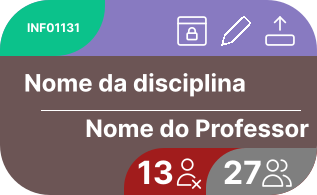
\includegraphics[width=\textwidth]{files/img/Desenvolvimento/Cartões/PadraoClassCards}
    \vspace{1mm} \vfill
    
\includegraphics[width=\textwidth]{files/img/Desenvolvimento/Cartões/Smaller ColapsadaClassCards}
  \end{minipage}
  \hfill
  \begin{minipage}{0.48\textwidth} \centering
    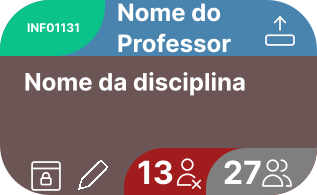
\includegraphics[width=\textwidth]{files/img/Desenvolvimento/Cartões/Professor SuperiorClassCards}
    \vspace{1mm} \vfill
    
\includegraphics[width=\textwidth]{files/img/Desenvolvimento/Cartões/SmallestClassCards}
  \end{minipage}
\end{MyCenteredFigure}
\begin{MyCenteredFigure}
  \caption{Protótipos de Caixas de Seleção}
  \label{fig:selects}
  \begin{minipage}{0.48\textwidth} \centering
    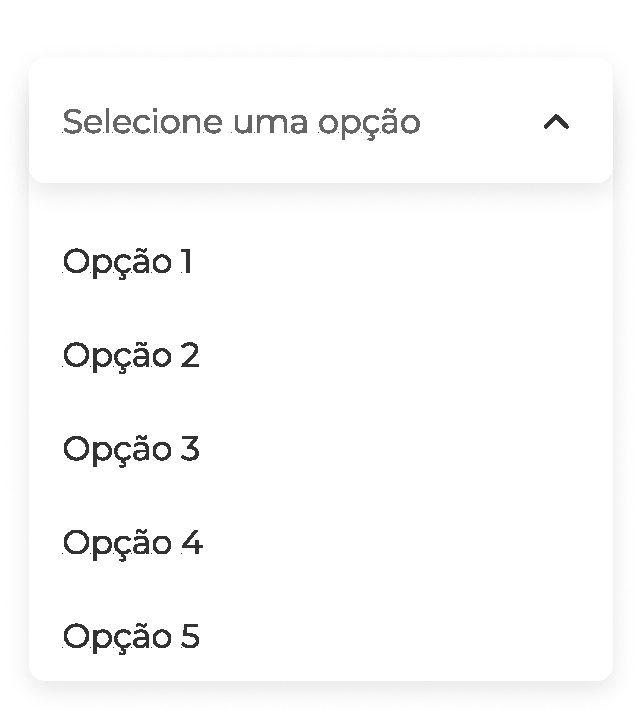
\includegraphics[width=\textwidth]{files/img/Desenvolvimento/SingleSelect.pdf}
  \end{minipage}
  \begin{minipage}{0.48\textwidth} \centering
    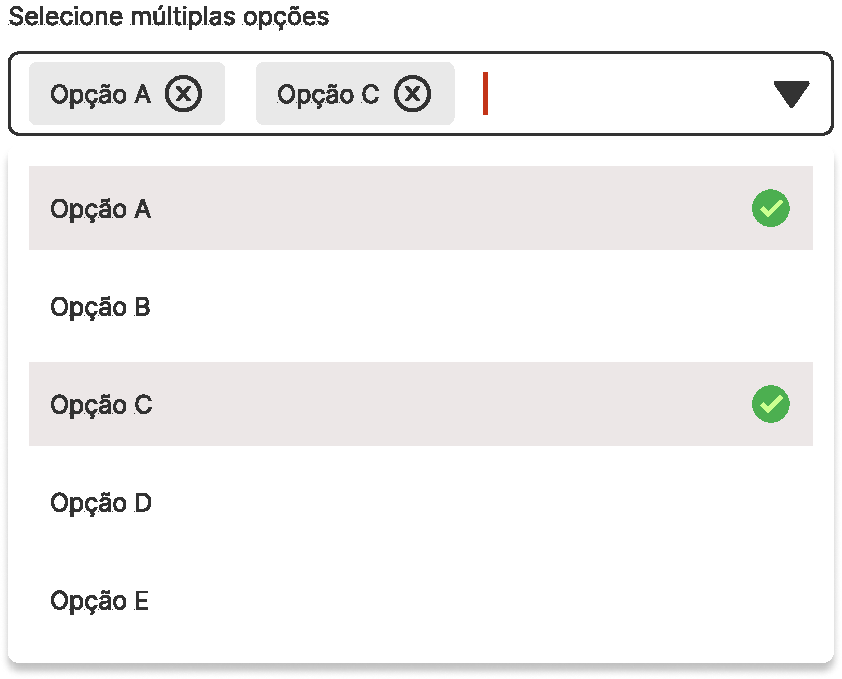
\includegraphics[width=\textwidth]{files/img/Desenvolvimento/MultiSelect.pdf}
  \end{minipage}
\end{MyCenteredFigure}

A criação de protótipos, seguindo a abordagem tomada por \cite{andre_interaction_2018}, se mostra como essencial para que se mantenha a constante satisfação por parte dos \textit{stakeholders} e quais mudanças sugerem ao desenvolvimento do projeto, assim reduzindo a necessidade de retrabalho ou de não alcance das expectativas do projeto.

Para este fim, foram feitos os designs iniciais usando o software de design \href{https://www.figma.com/}{Figma}. Algumas telas principais foram concebidas. A primeira, e principal, é a ilustrada pela \autoref{fig:main} que permite que o usuário arraste a turma até o horário desejado. A turma ao qual este horário se refere pode ser definida na parte lateral direita.

\begin{MyCenteredFigure}[htbp]
  \caption{Página principal do sistema}
  \label{fig:main}
  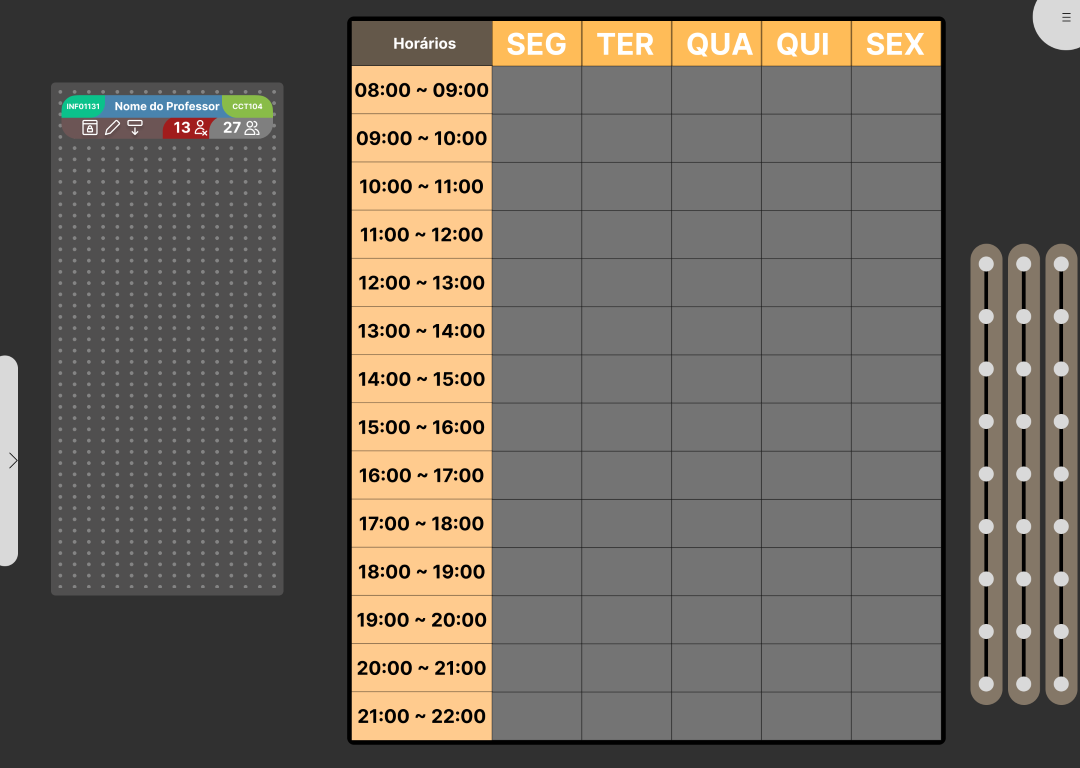
\includegraphics[width=0.8\textwidth]{files/img/Prototipo/Medio/main}
\end{MyCenteredFigure} % Main

Em seguida, temos a tela base para seleção de dados que deseja-se modificar, ilustrada pela \autoref{fig:CRUD_main}, podendo ser de turmas, salas, disciplinas, professores, alunos.

Cada um desses tendo sua própria página de criação, leitura, edição ou deleção de dados.

\begin{MyCenteredFigure}
  \caption{Página principal de modificação dos dados}
  \label{fig:CRUD_main}
  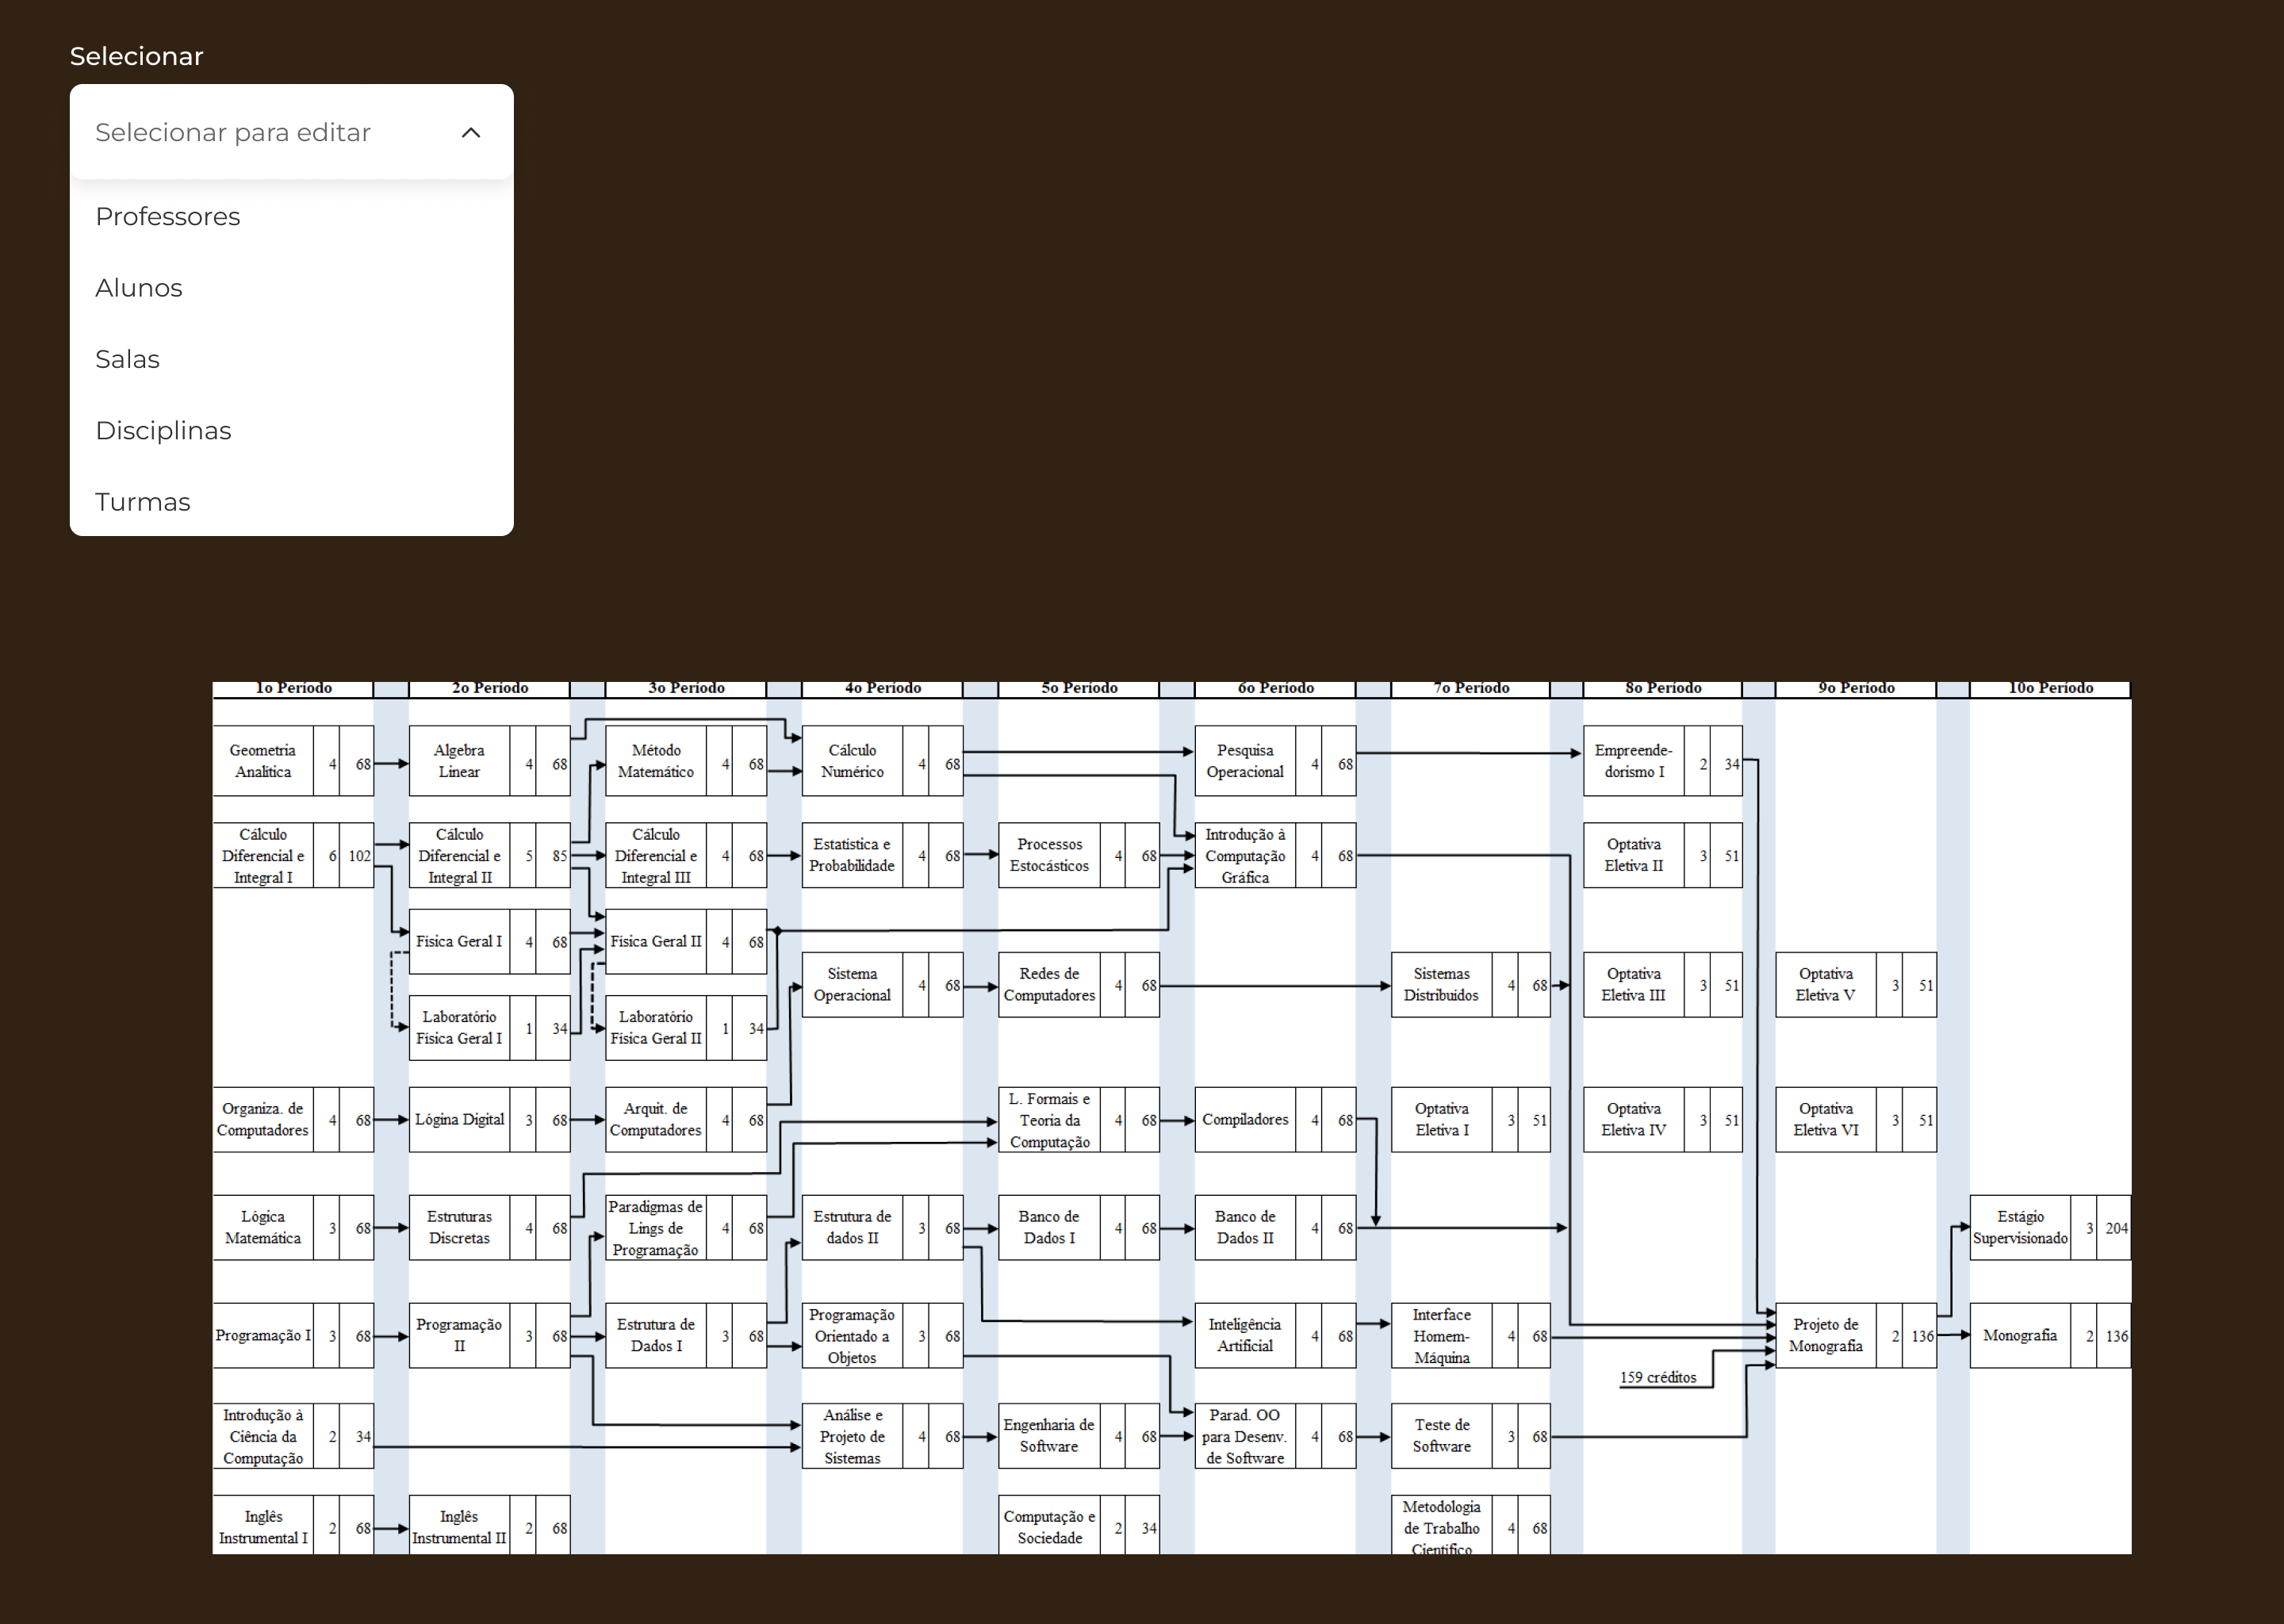
\includegraphics[width=0.8\textwidth]{files/img/Prototipo/Medio/CRUD_main}
\end{MyCenteredFigure} % CRUD_main

Quanto às salas, temos a sua alocação atual baseado no ano e semestre. Nessa página pode-se também registrar algumas características da sala, como a quantidade de cadeiras e computadores, e se possui monitor, projetos, quadro de giz e quadro branco. Um exemplo de sala ainda sem turmas alocadas é representado na \autoref{fig:CRUD_salas-vazias}.

\begin{MyCenteredFigure}
  \caption{Página de modificação das informações de salas}
  \label{fig:CRUD_salas-vazias}
  \includegraphics[width=0.8\textwidth]{files/img/Prototipo/Medio/CRUD_salas-vazias}
\end{MyCenteredFigure} % CRUD_salas-vazias

Na página dos alunos, pode-se cadastrar novos alunos informando o seu ano de entrada e a sua matrícula. Abaixo temos a visualização da grade, onde pode-se classificar cada uma das disciplinas como aprovada, reprovada e cursando. O exemplo da \autoref{fig:CRUD_alunos} mostra a grade de um aluno inscrito em 2019.1.

\begin{MyCenteredFigure}
  \caption{Página de modificação das informações de alunos}
  \label{fig:CRUD_alunos}
  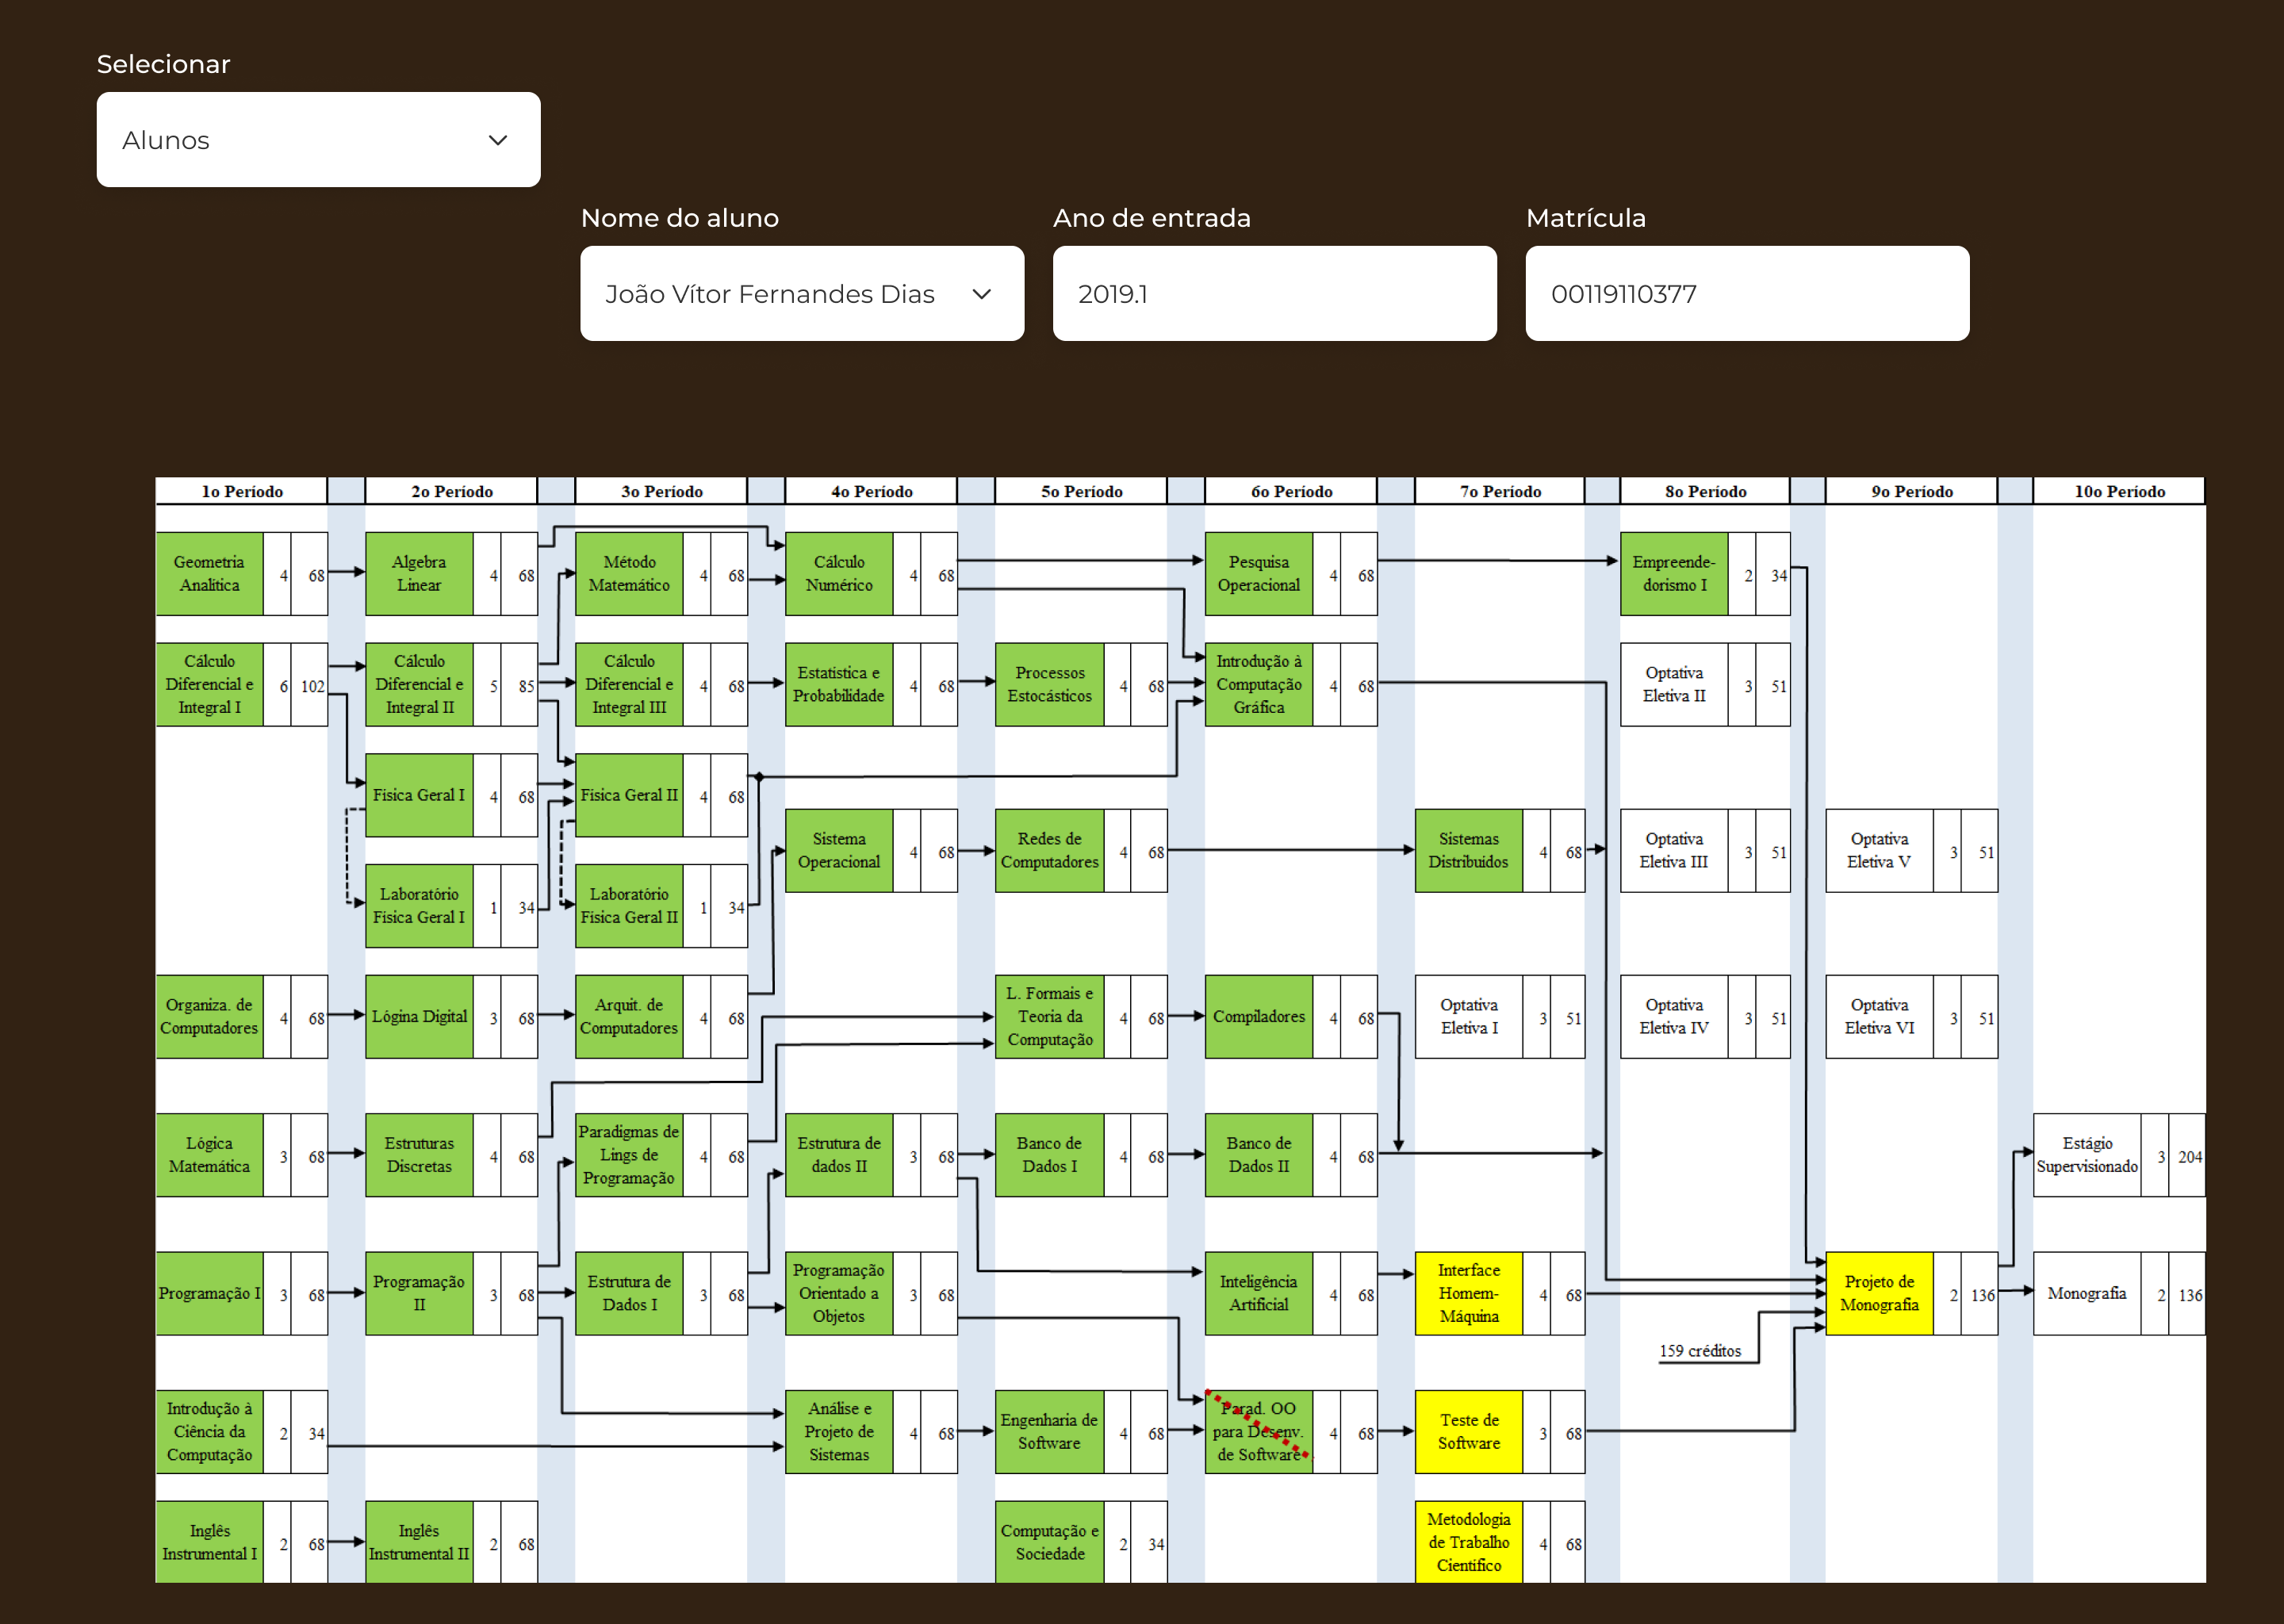
\includegraphics[width=0.8\textwidth]{files/img/Prototipo/Medio/CRUD_alunos}
\end{MyCenteredFigure} % CRUD_alunos

Podemos também definir nas disciplinas qual seu código e nome, e o seu período esperado segundo a ementa. Informamos quais cursos a possuem em suas ementas, quais seus pré-requisitos, os professores que a ministram e quais requisitos a mesma possui em relação às características de sala. A \autoref{fig:CRUD_disciplinas} mostra a página de modificação de disciplinas.

\begin{MyCenteredFigure}
  \caption{Página de modificação das informações de disciplinas}
  \label{fig:CRUD_disciplinas}
  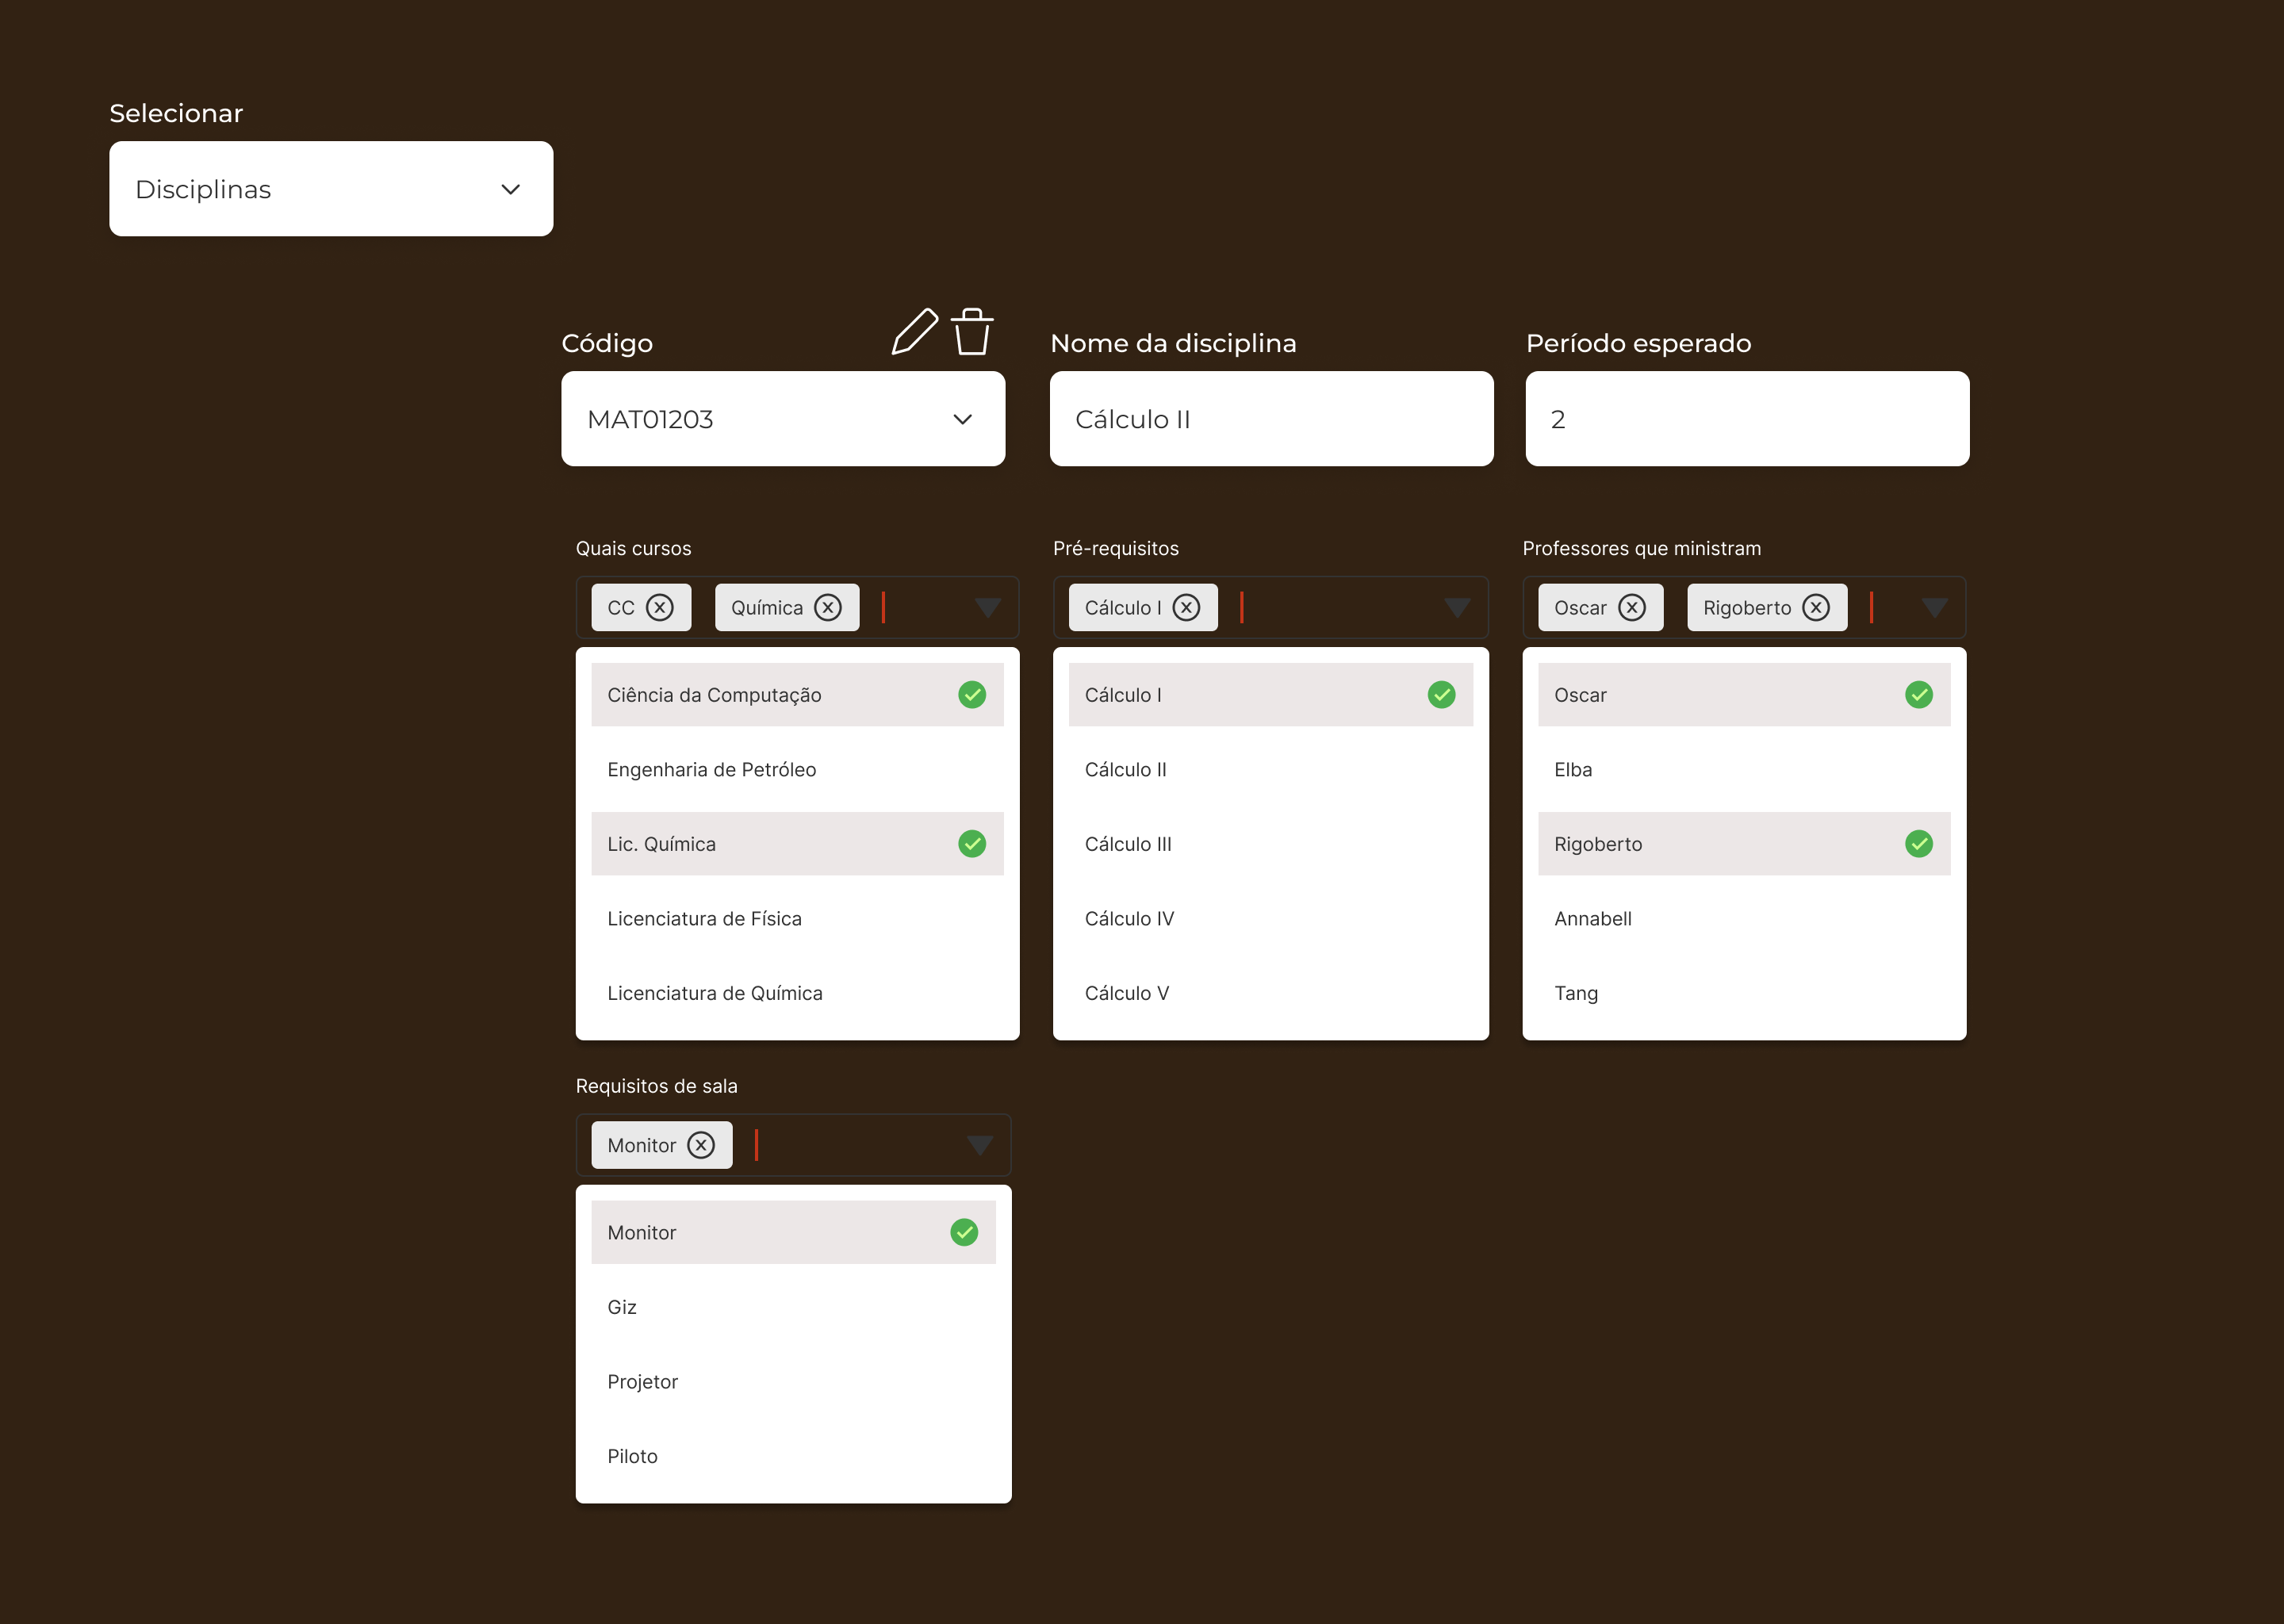
\includegraphics[width=0.8\textwidth]{files/img/Prototipo/Medio/CRUD_disciplinas}
\end{MyCenteredFigure} % CRUD_disciplinas

Na seção de professores, temos a relação de disciplinas que os mesmos estão passíveis de ministrar, e também quais são suas preferências de horários ao longo da semana. A \autoref{fig:CRUD_professores} mostra a página de modificação de professores.

\begin{MyCenteredFigure}
  \caption{Página de modificação}
  \label{fig:CRUD_professores}
  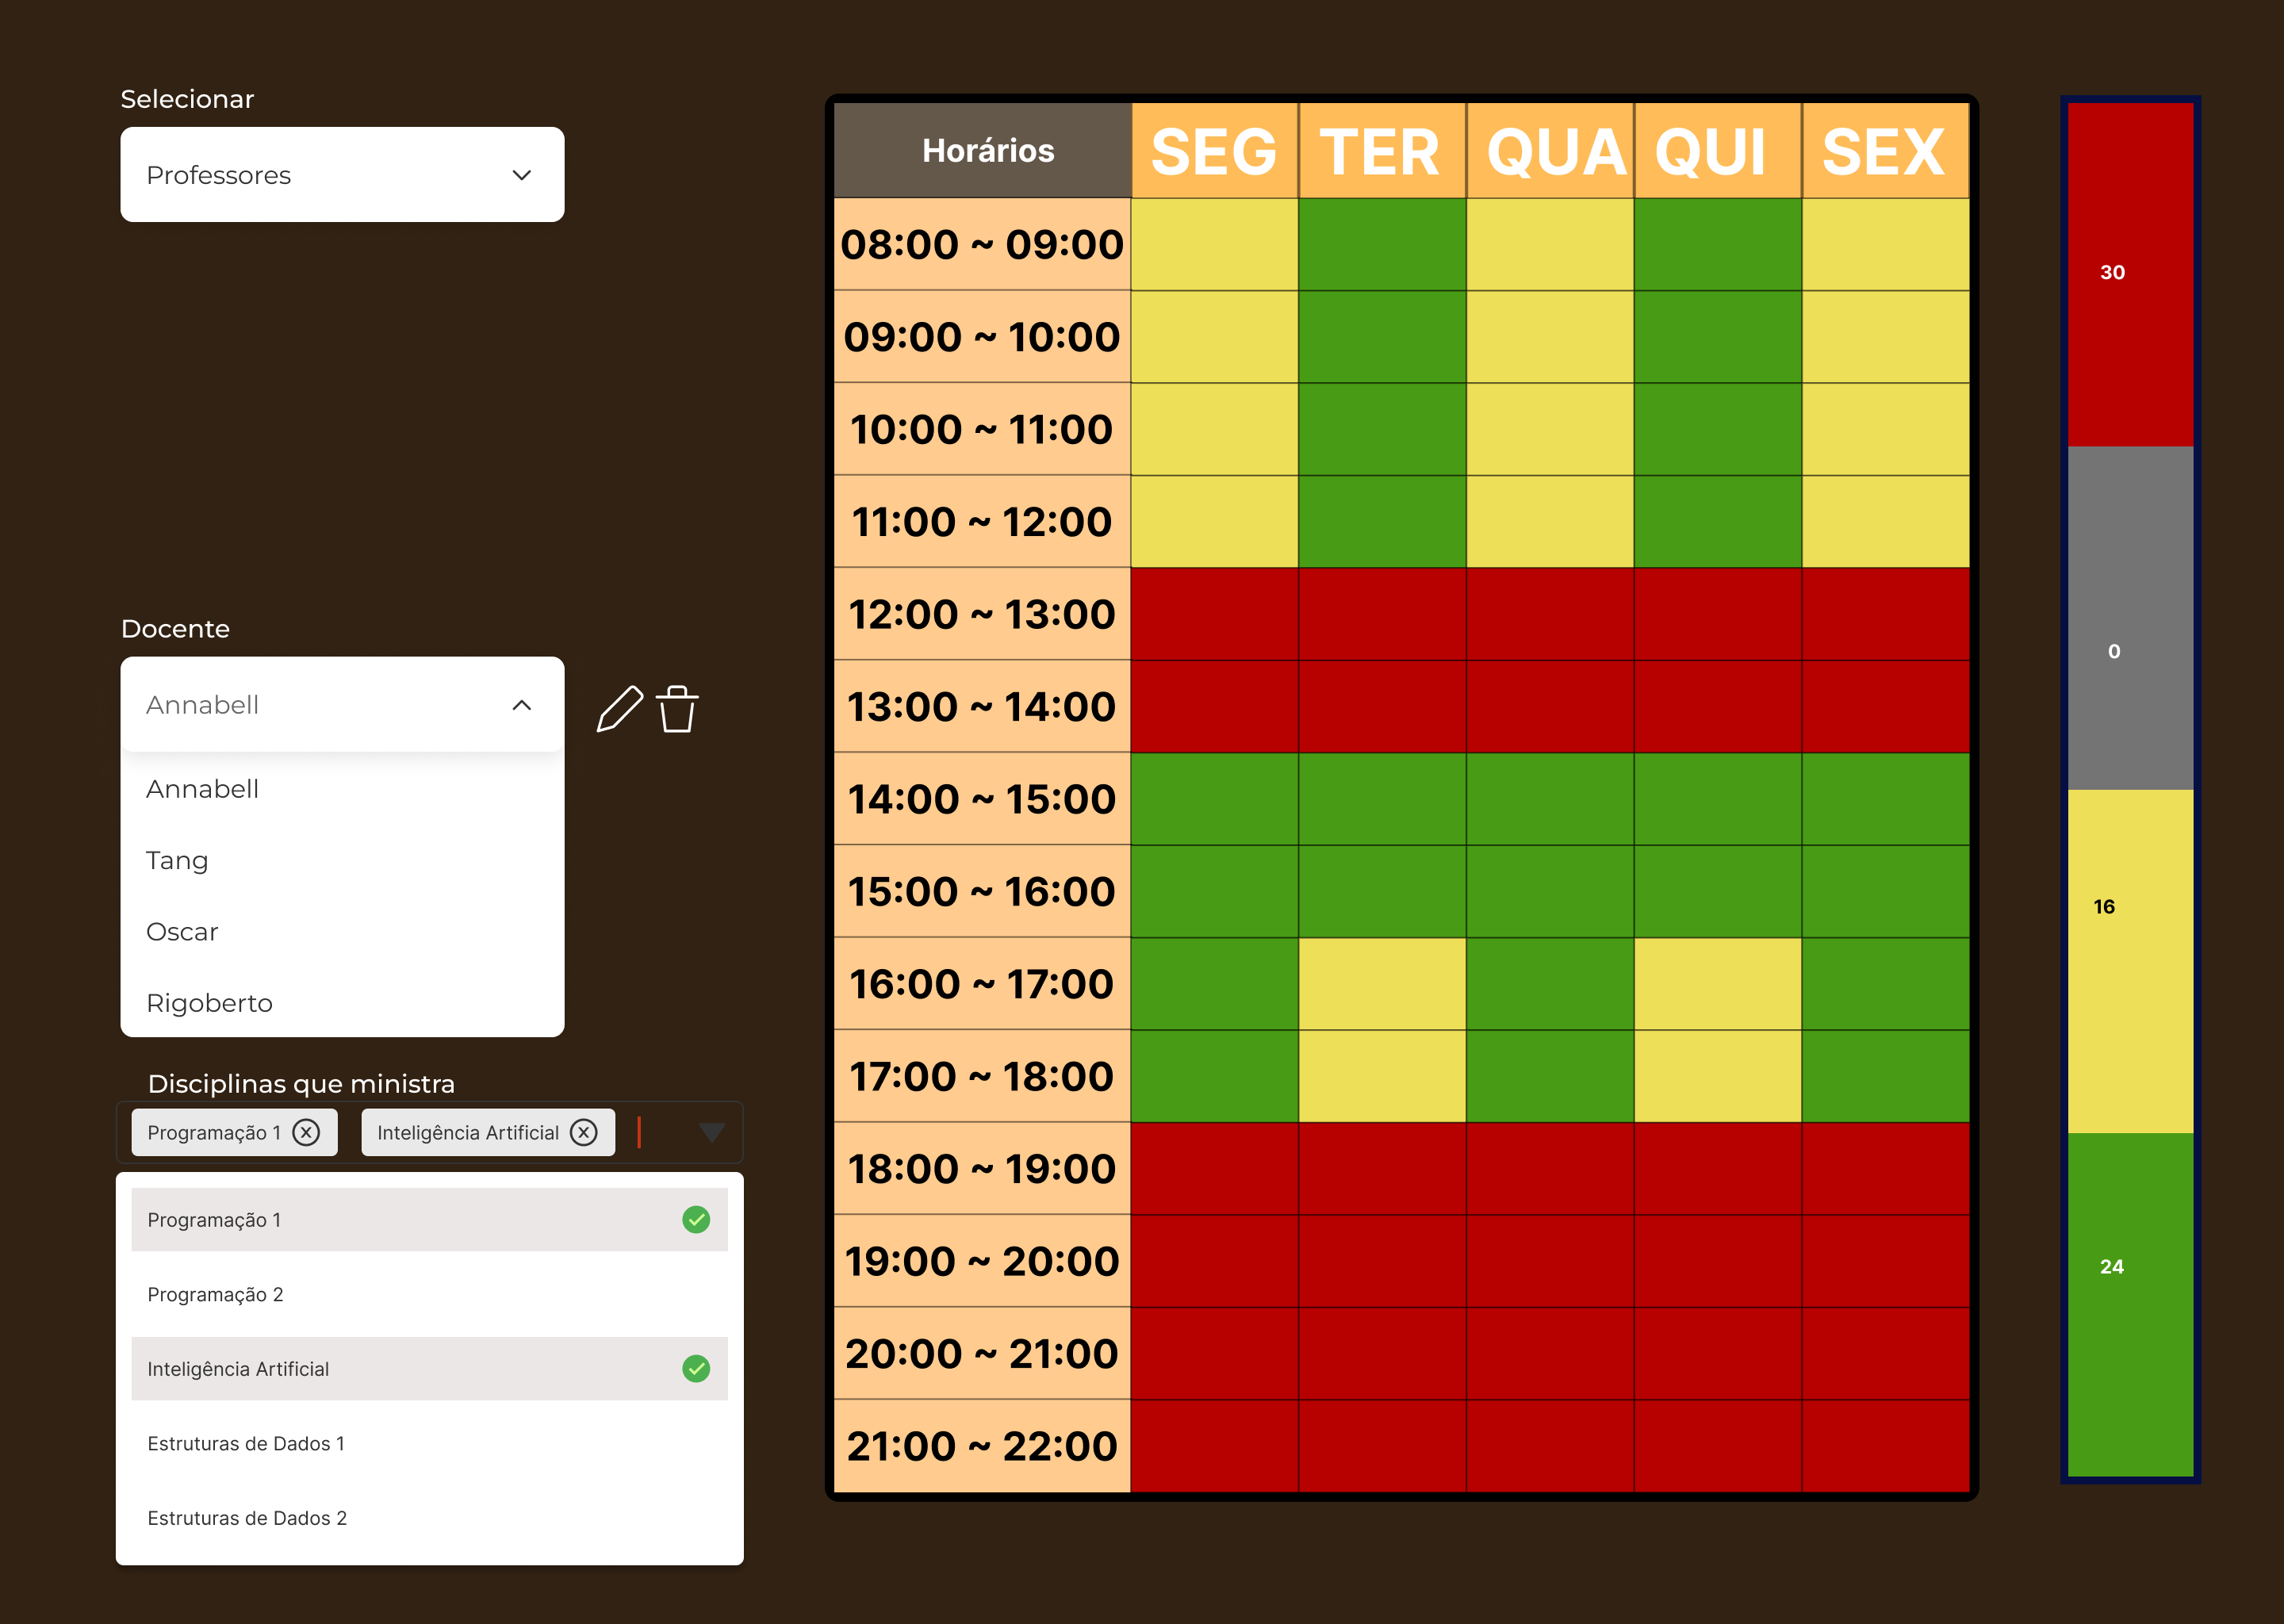
\includegraphics[width=0.8\textwidth]{files/img/Prototipo/Medio/CRUD_professores}
\end{MyCenteredFigure} % CRUD_professores

Por fim, temos a junção de todas as informações registradas acima. Nela, podemos informar em quais horários, dias e em que sala, a turma estará alocada, além de informar qual professor a lecionará e a qual disciplina ela se refere.

Na imagem temos um exemplo das ilustrações de níveis de alerta, informando que o tempo de duração do segundo dia de aulas não condiz com a preferência pessoal do professor selecionado, e que na primeira sala estão ocorrendo conflitos. Conflitos esses ressaltados nos nomes dos alunos que demandam tal disciplina, como pode ser visto na \autoref{fig:CRUD_turmas}.

\begin{MyCenteredFigure}
  \caption{Página de modificação das informações de turmas}
  \label{fig:CRUD_turmas}
  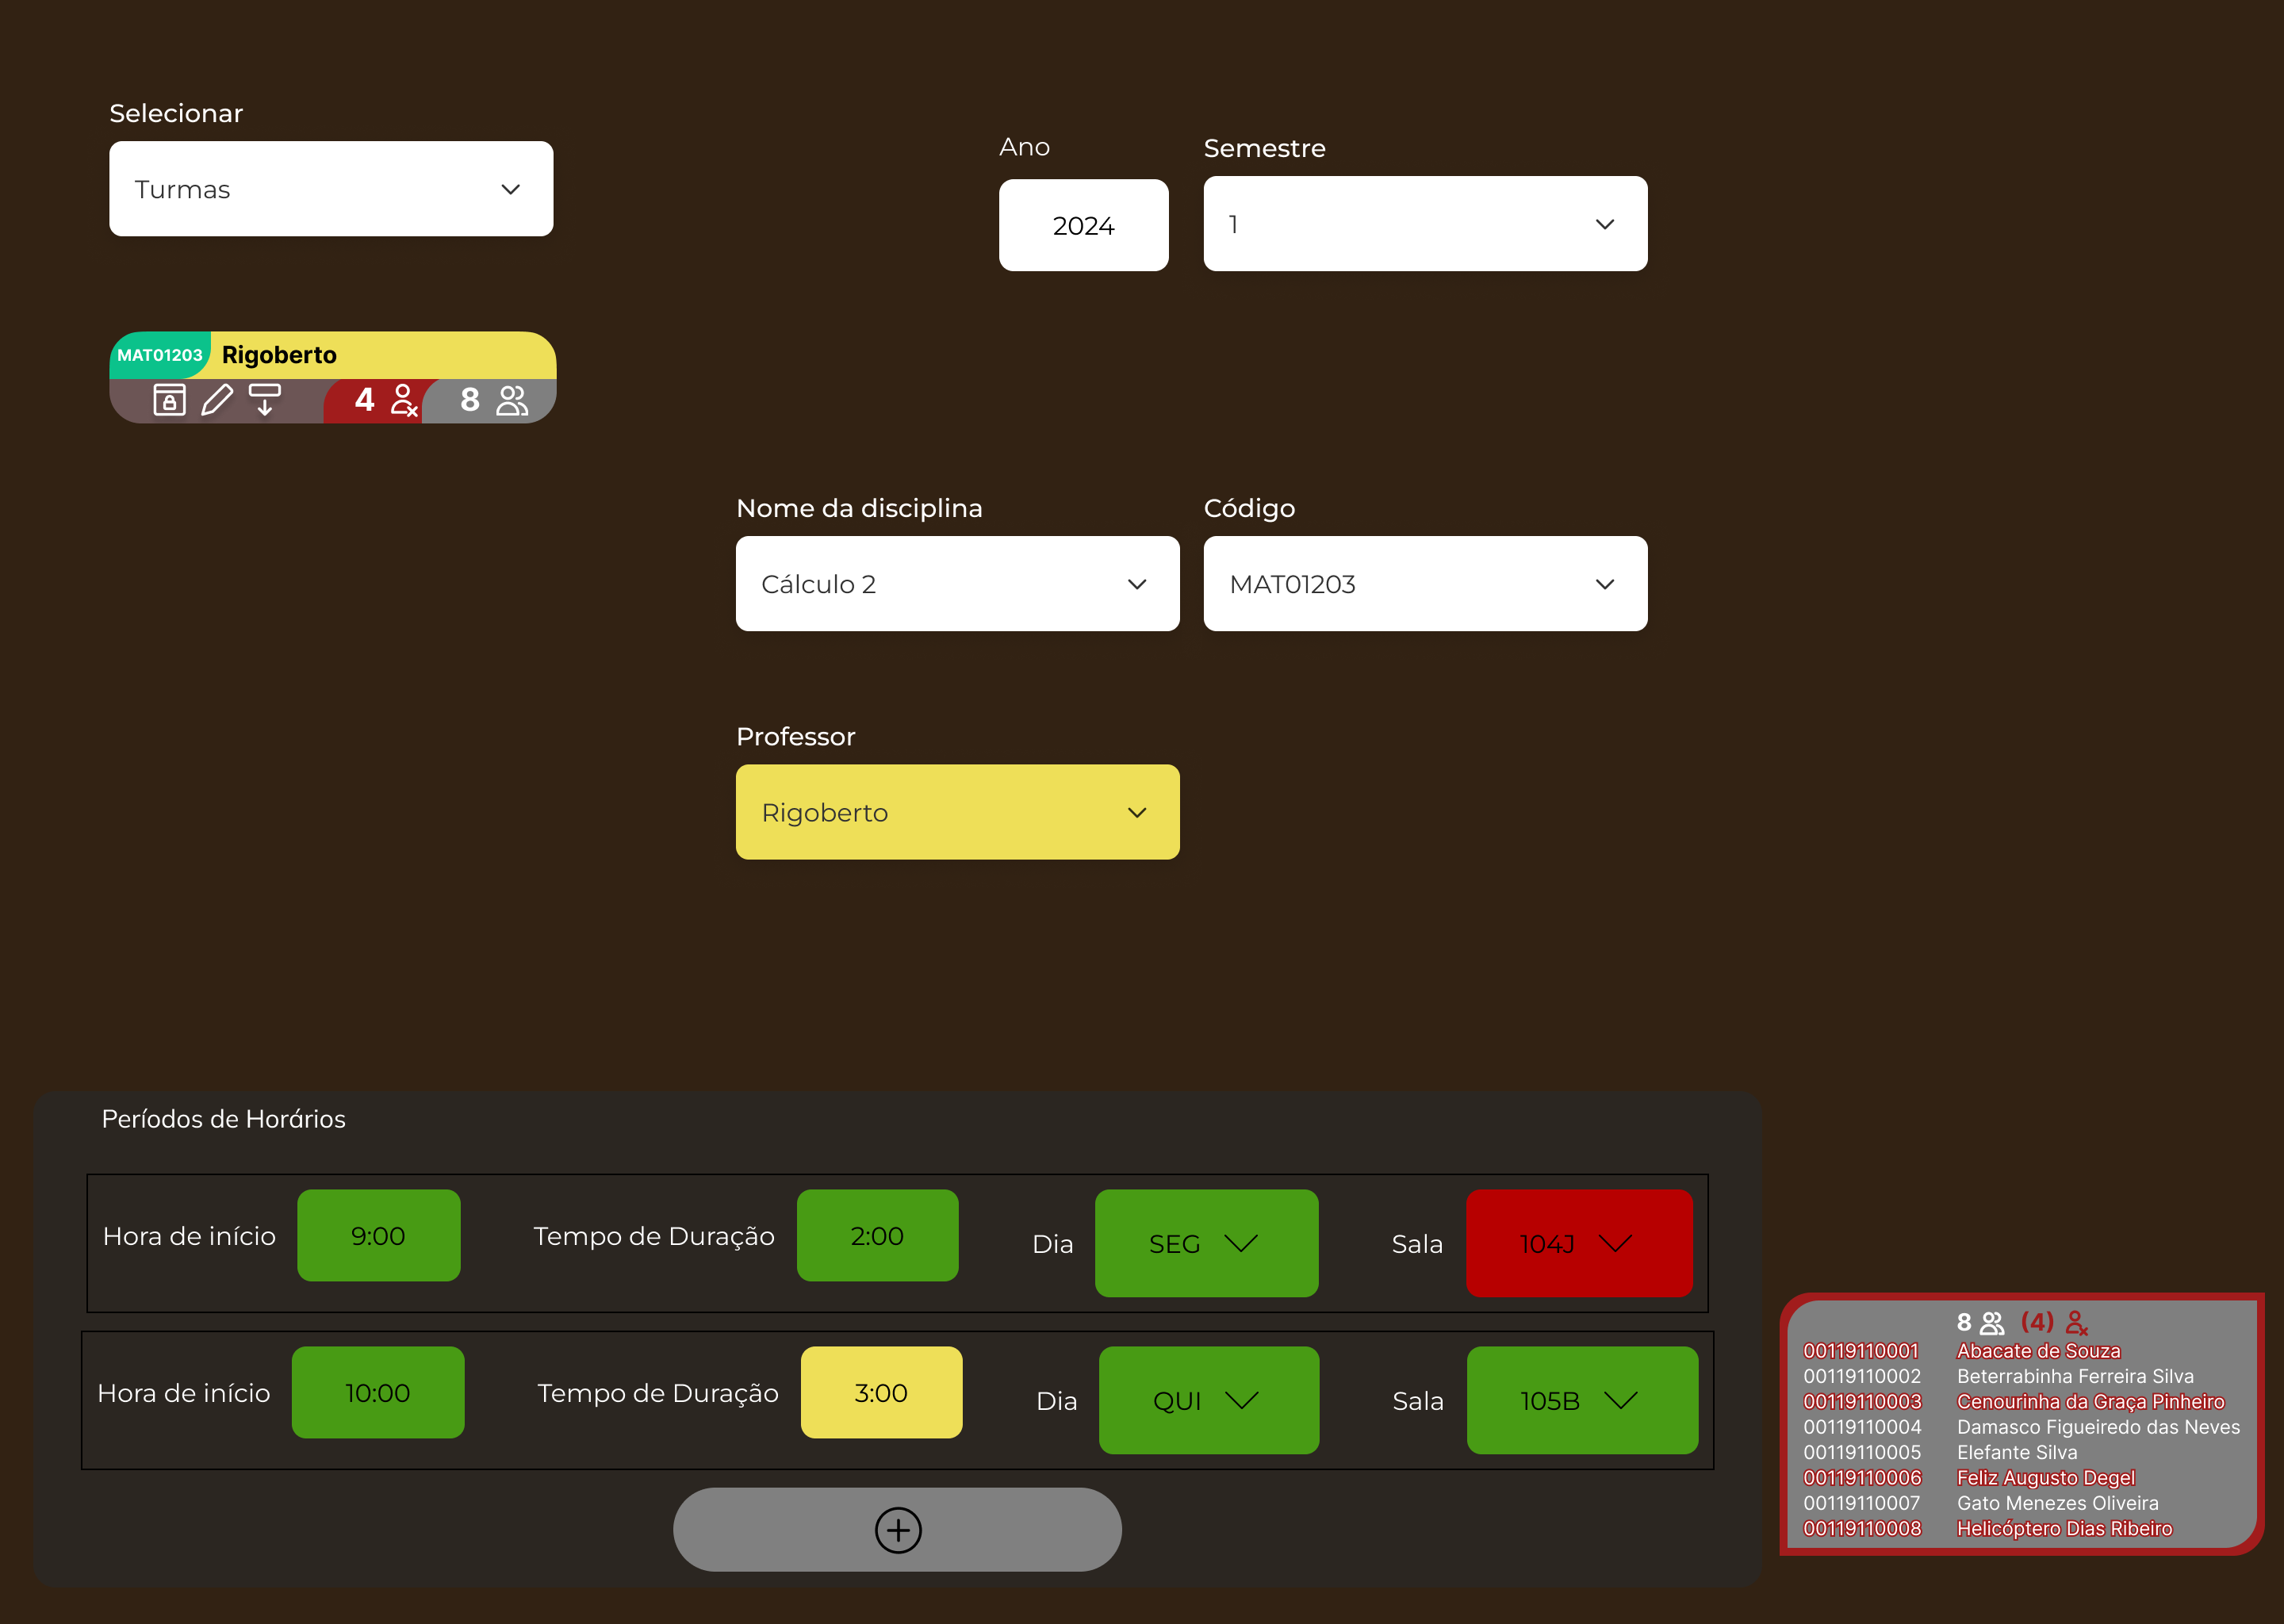
\includegraphics[width=0.8\textwidth]{files/img/Prototipo/Medio/CRUD_turmas}
\end{MyCenteredFigure} % CRUD_turmas

\section{Modelo de Banco de Dados} \label{ModelagemBD} % ### 5.4. Modelo de Banco de Dados

Considerando as informações necessárias para o presente trabalho, e também o preparo de campo para potenciais aplicações futuras, foi elaborado um diagrama conceitual de banco de dados, que pode ser visto na Figura \ref{fig:DiagramConceitual}.

\begin{figure}[htbp]\centering
  \caption{\label{fig:DiagramConceitual} Diagrama Conceitual do banco de dados}
  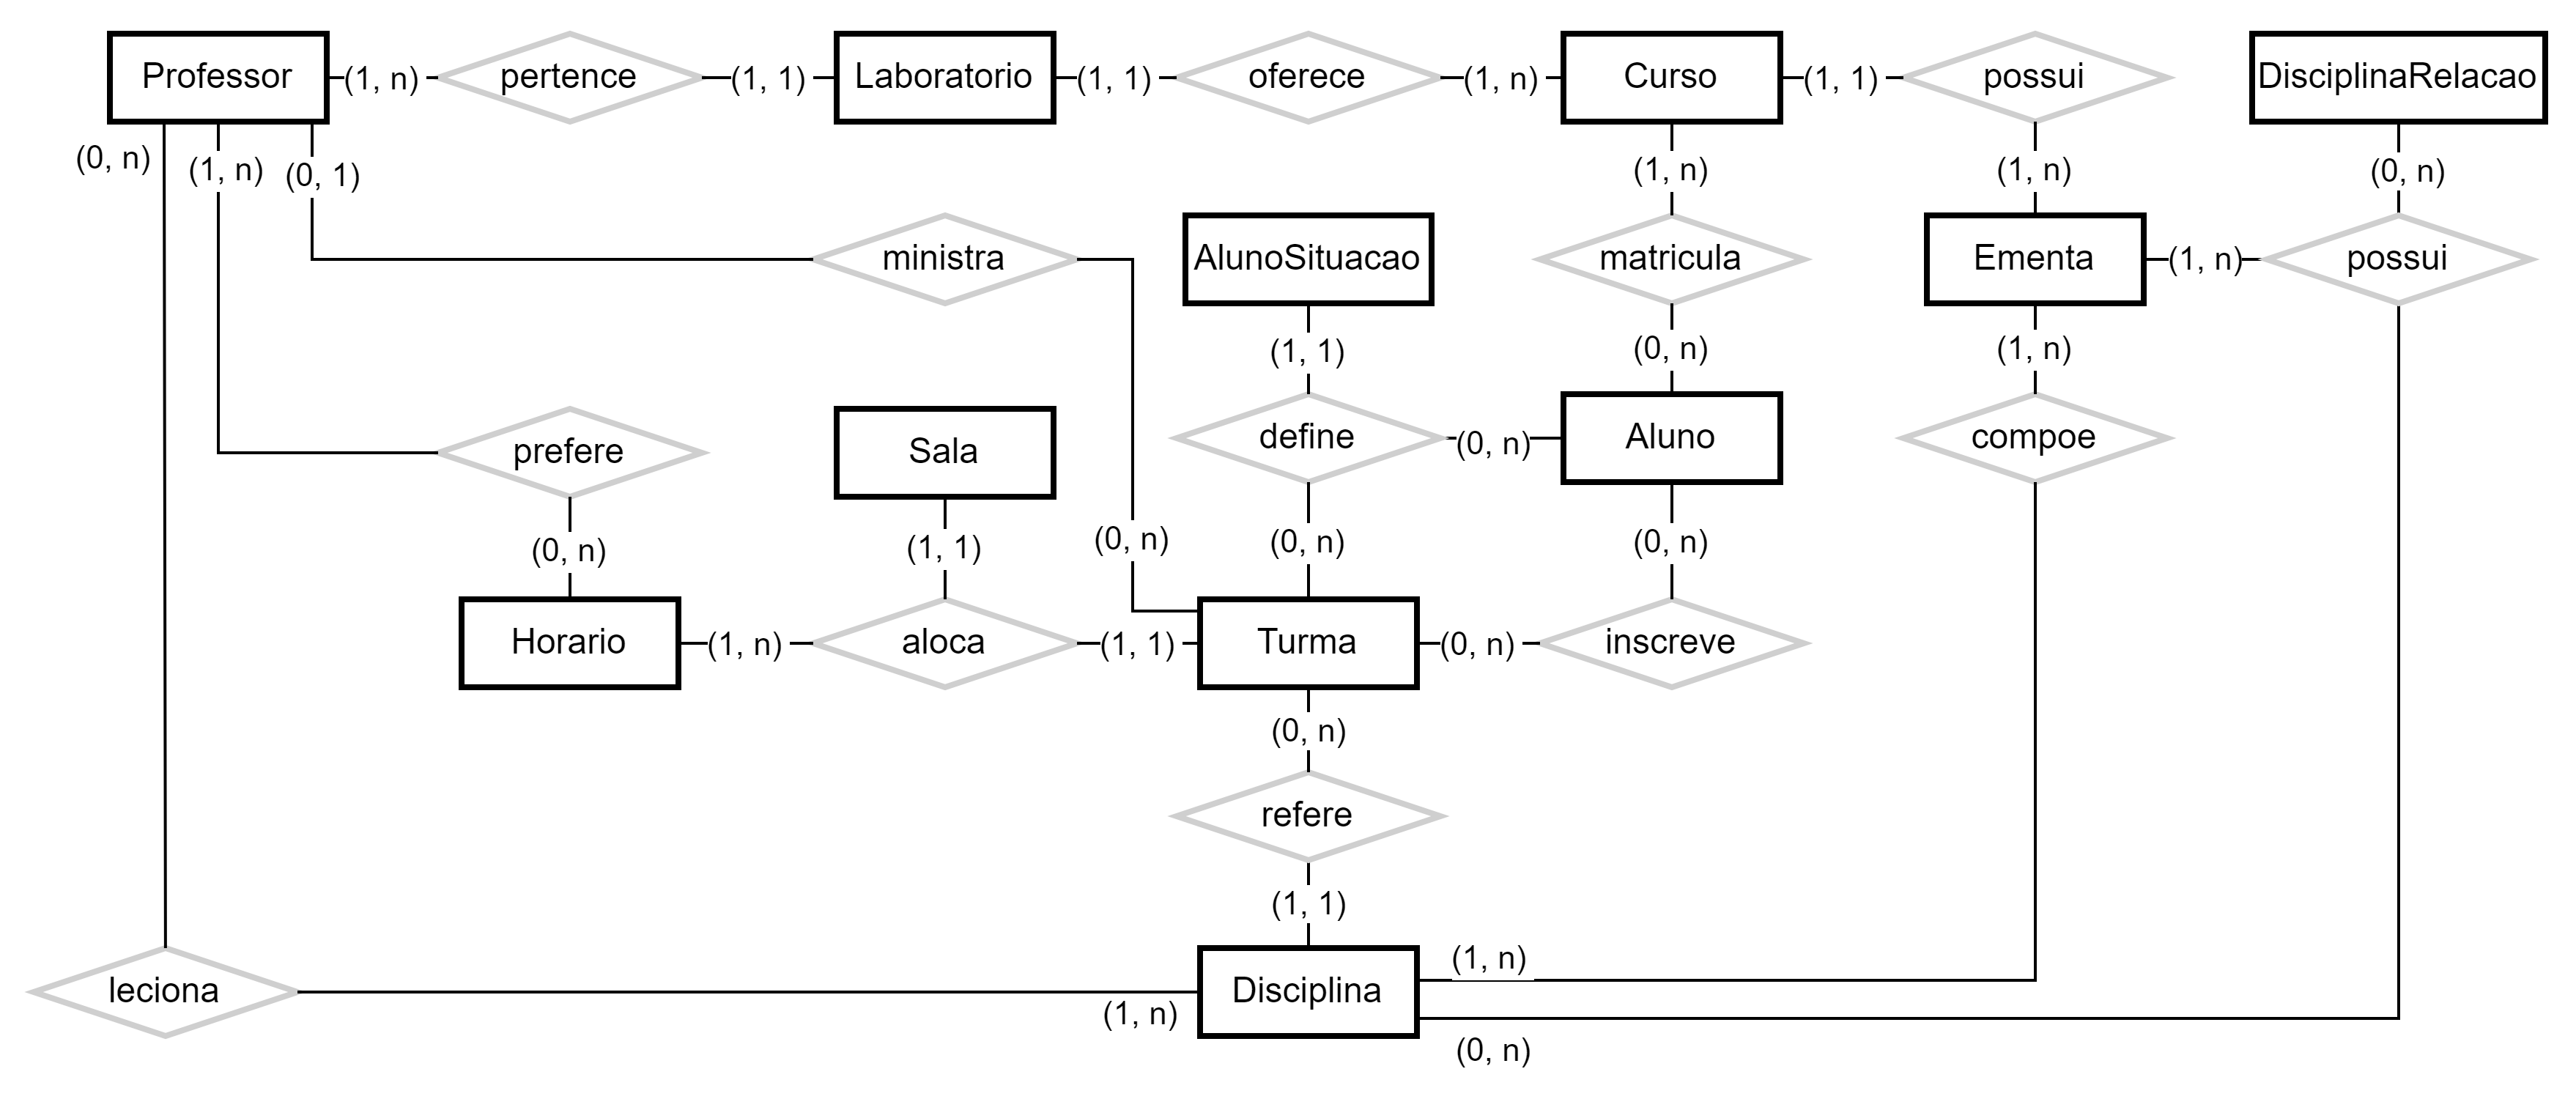
\includegraphics[scale=0.2]{files/img/DiagramaConceitual/DiagramaConceitualBranco.png}
  \legend{Fonte: o autor}
\end{figure} % Diagrama Conceitual

O diagrama conceitual foi elaborado utilizando a ferramenta \href{https://www.drawio.com/}{draw.io} citada na metodologia e ilustra as relações entre diversas entidades presentes na realidade da UENF. O emaranhamento presente no diagrama ilustra a complexidade envolvida na criação de uma grade horária, onde diversas entidades se relacionam entre si.

Como principais apontamentos, podemos citar a parte principal do modelo que é a alocação de turmas. Ela, como já descrito, envolve a correlação entre alunos de diferentes cursos, professores, disciplinas, salas e horários. Além disso, também é possível notar a presença de entidades que não são diretamente relacionadas à alocação de turmas, mas que podem se mostrar úteis, como a relação entre professores e laboratórios, e a de disciplinas e ementas.

Embora o diagrama apresente uma visão mais completa de todas as interconexões possíveis, é importante ressaltar que o presente trabalho foca primordialmente na alocação das turmas para o curso de Ciência da Computação, e que a implementação do banco de dados será feita de forma a atender a essas necessidades, fazendo então uso de uma parte do diagrama conceitual.

% Tendo isso em vista, o modelo conceitual reduzido para o presente trabalho pode ser visto na Figura \ref{fig:DiagramConceitualReduzido}.

% \begin{figure}[htbp]\centering
%   \caption{\label{fig:DiagramConceitualReduzido} Diagrama Conceitual reduzido para o presente trabalho}
%   \includegraphics[scale=0.2]{files/img/DiagramaConceitual/DiagramaConceitualReduzidoBranco.png}
%   \legend{Fonte: o autor}
% \end{figure} % Diagrama Conceitual reduzido

Neste modelo, mais enxuto, temos apenas as entidades principais, onde temos uma turma de determinada disciplina, ministrada por um professor e que ocorre em uma sala em um determinado horário.

\subsection{Diagrama de Entidade e relacionamento} % ### 5.4.1. Modelo Relacional

% Com isso, restamos o diagrama de Entidade e Relacionamento (DER) que pode ser visto na Figura \ref{fig:DER}.

% \begin{figure}[htbp]\centering
%   \caption{\label{fig:DER} Diagrama de Entidade e Relacionamento}
%   \includegraphics[scale=0.2]{files/img/DER/DERBranco.png}
%   \legend{Fonte: o autor}
% \end{figure} % Diagrama de Entidade e Relacionamento

Neste diagrama vemos as entidades principais, que são \textit{Turmas}, \textit{Disciplinas}, \textit{Professores}, \textit{Horários} e \textit{Salas}. As propriedades escolhidas para cada entidade são compostas por uma mistura de critérios. Por exemplo, o nome do professor, o código da disciplina, e a junção de código e bloco auxiliam primordialmente na identificação real dos professores, disciplinas e salas. Já as informações ``período'', ``apelido'' e ``comment''...

E também é notável a presença da entidade \textit{Alunos}, que se apresenta desacoplado das demais entidades. O motivo para isso é que, embora os alunos façam parte do processo de alocação de turmas, ao longo do desenvolvimento, o desenvolvimento de funcionalidades envolvendo os alunos...

\section{História do desenvolvimento} % ### 5.5.1. História do desenvolvimento

%% Acho que vai ficar mais fácil assim

Após a elaboração dos protótipos com o Figma, e da conceitualização diagramática do banco de dados, o desenvolvimento do sistema foi iniciado. Por maior familiaridade com a linguagem e considerando que é uma das mais utilizadas no mercado para desenvolvimento web [buscar referência], foi escolhida a linguagem JavaScript, utilizando a biblioteca React para a criação dos componentes visuais, ou seja, o front-end, e o Node.js para a criação do back-end e a criação de um servidor local que permitiria visualizar as mudanças no código em tempo real.

% Perguntar pra quem sabe, sobre qual é o real papel do Node.js

\subsection{Primeira versão} % ### 5.5.2. Primeira versão

A primeira versão do sistema foi desenvolvida em um ambiente local, com o objetivo de se aproximar ao máximo das páginas previstas no protótipo. Para isso, foi utilizada a biblioteca React Router para a navegação entre as páginas, e a biblioteca React Select para as caixas de seleção.

\subsubsection{Banco de Dados primitivo}

Os dados contidos no sistema foram inicialmente armazenados em arquivos JSON, que eram importados diretamente para o código. Isso foi feito para que fosse possível visualizar o funcionamento do sistema sem a necessidade de um banco de dados real. A partir disso, foi possível visualizar o funcionamento do sistema e realizar testes de usabilidade. Em contrapartida, os dados disponíveis não eram modificáveis, tendo apenas a possibilidade de leitura e mutação temporária, visto que após recarregar ou mudar de página, as mudanças eram perdidas.

Nesse método, cada entidade era armazenada em um arquivo JSON separado, contendo esse um array de objetos, onde em cada objeto haviam as chaves, representando as propriedades da entidade, e os valores, representando os dados da entidade.

Como nesta dinâmica não havia uma forte correlação entre os dados, o frontend acabava sendo o responsável por unir todas as informações. Assim, por exemplo, para se obter a lista de professores de uma turma, era necessário importar todos os professores, todas as turmas, e então, a partir do nome do professor alocado àquela turma, buscar na listagem dos professores qual era o professor que correspondia àquele nome, para então agregar as informações.

\subsubsection{Funcionalidades iniciais}

Nessa primeira versão, algumas funcionalidades já começaram a ser esboçadas, principalmente as funcionalidades CRUD (Create, Read, Update, Delete) para as entidades principais do sistema. Embora, como já dito, os dados não fossem persistentes, foi possível visualizar o funcionamento das funcionalidades de criação e leitura de turmas, professores, disciplinas, salas e horários.

Nessa versão, também foi implementada uma checagem bruta de conflitos por alocação simultânea de professores em mais de uma turma e a checagem da quantidade de demanda de alunos em relação à capacidade das salas. Uma descrição mais detalhada das funcionalidades de conflitos está presente \hyperref[Conflitos]{adiante}.

Além dessas funcionalidades que se mantiveram até a conclusão do sistema, também foram desenvolvidas funcionalidades que não obtiveram o mesmo êxito e que foram deixadas de lado ao decorrer do caminhar. Dentre elas, podemos citar a definição de níveis de preferência de horários para professores, a definição das características especiais das salas, e o andamento dos alunos em relação às disciplinas. Houveram também outras que nem chegaram a ser desenvolvidas, como a realocação de turmas através de um sistema de arrastar e soltar e o uso de heurísticas para a realocação de turmas.

\subsubsection{GitHub Pages}

Após o desenvolvimento local, como forma de viabilizar o acesso ao sistema por parte de outros usuários, foi feito o \textit{deploy}, ou seja, foi feito o upload do sistema para um servidor online. Para isso, foi utilizado o serviço GitHub Pages que, por ser gratuito e de fácil utilização, foi a escolha mais adequada para o momento. O sistema pode ser acessado através do link \url{https://jvfd3.github.io/timetabling-UENF/}.

\subsection{Segunda versão} % ### 5.5.3. Segunda versão

Utilizando do feedback quanto aos resultados entregues na primeira versão, alguns pontos de melhoria foram identificados, sendo um deles, e o mais importante: o planejamento. Na primeira abordagem, o desenvolvimento foi feito seguindo notas e ideias soltas, sem um planejamento prévio, o que resultou em um sistema que, embora funcional, não atendia a todas as necessidades propostas. E ia além: exibia funcionalidades que não eram de todo necessárias, ou melhor dizendo, têm menor prioridade do que muitas outras.

% Mesmo com esta nova dinâmica, outras funcionalidades foram deixadas de lado. Uma das que foram deixadas de lado foi a possibilidade de fixar certas informações. A proposta era que, certas disciplinas como Cálculo e Álgebra que são ofertadas para múltiplos cursos, pudessem ser fixadas em horários específicos, para que simplificasse aos coordenadores dos cursos a alocação de turmas.

\subsubsection{GitHub Projects}

Com isso, utilizando o GitHub Projects, foi organizado uma tabela de tarefas, onde foram unificadas as diversas anotações e ideias, antes soltas. A partir disso, foi possível visualizar o que era mais importante e o que poderia ser deixado de lado.

% [ADICIONAR IMAGEM DA TABELA BONITINHA: https://github.com/users/jvfd3/projects/3]

Tendo este novo sistema de tarefas em prática, foi possível tranquilizar a mente quanto ao conflito entre as funcionalidades que precisavam ser desenvolvidas, as que já estavam prontas, as que poderiam ter melhorias e quais se desejava implementar no futuro.

As tarefas foram inicialmente divididas em três principais categorias: \textit{Status}, \textit{Pages} e \textit{Sequence}. O \textit{Status} reflete o andamento da tarefa, se ela está disponível, em andamento, ou concluída. O \textit{Pages} reflete em qual página do sistema a tarefa se encontra, e o \textit{Sequence} reflete a ordem de prioridade da tarefa.

\subsubsection{Permanência dos dados}

Tendo agora uma rota mais clara a ser seguida, o desenvolvimento foi retomado. Uma das características mais marcantes e ainda não atribuídas ao sistema era a manutenção dos dados. Para exemplificar o funcionamento geral da permanência dos dados, consideremos o uso de uma \textit{REST API} utilizando de 4 ``camadas'': A. o frontend; B. os endpoints; C. as funções de execução; D. o banco de dados.

% [Usar diagrama para ilustrar]

O \textbf{frontend} é a interface do sistema, onde o usuário interage com o sistema. Ele se encontra em duas formas: a primeira é o chamado ``em produção'', que é o sistema que o usuário final acessa, e a segunda é o chamado ``em desenvolvimento'', que é o sistema que o desenvolvedor acessa para realizar as modificações necessárias. Ambas precisam se comunicar com o backend para realizar as quatro operações básicas no banco de dados (criação, leitura, atualização e deleção) por sobre as entidades existentes (turmas, professores, disciplinas, salas, etc.). Elas assim o fazer ao enviar requisições HTTP (GET, POST, PUT e DELETE), contendo pacotes de informações em formato JSON para os \textbf{endpoints}.

Os \textbf{endpoints} são as rotas que o backend disponibiliza para a recepção das requisições HTTP. Eles são responsáveis por encaminhar as requisições recebidas. Se funcionamento é simples: rotear as requisições recebidas junto com sua carga útil. Para tanto, as rotas criadas refletem diretamente a qual entidade do banco de dados a requisição se refere, sendo então assim sabido qual \textbf{função} deve ser executada.

As \textbf{funções} são as responsáveis por executar as operações no banco de dados. Elas processam o pacote de informações recebido, e então realizam a operação desejada no \textbf{banco de dados}.

O \textbf{banco de dados} recebe a requisição, processa a operação, e então retorna o status da operação. Esse retorno é então repassado camada por camada, até chegar ao frontend, onde o usuário final pode visualizar o resultado da operação.

\textbf{Resumidamente}: O \textbf{frontend} envia uma requisição HTTP com uma carga de informações a um \textbf{endpoint}, que encaminha a requisição a uma \textbf{função} específica que executa uma operação no \textbf{banco de dados}, assim retornando o status da operação ao frontend.

\paragraph*{\href{https://jsonbin.io/}{JSONBin}}

Como até então os dados estavam armazenados em formato JSON, imaginou-se que a melhor forma de persistir os dados seria através de um banco de dados que lidasse com JSON, e o escolhido foi o JSONBin.

Esta plataforma permite a criação de \textit{bins}, que são basicamente coleções de dados em formato JSON. A partir disso, é possível realizar requisições HTTP para a leitura, escrita, atualização e remoção dos dados. A utilização do JSONBin foi feita através de requisições HTTP usando o objeto \textit{XMLHttpRequest} do JavaScript, e a comunicação entre o frontend e o JSONBin foi feita através de \textit{tokens} de acesso.

Com isso, se tornou possível ler e atualizar os dados de forma remota, e assim, manter os dados mesmo após a recarga da página. Embora cumprisse com o que promete e o que era desejado, o JSONBin não se mostrou a melhor escolha para o sistema, visto que a sua utilização não performou tão bem quanto se esperava. Não se sabe se foi por inexperiência ou por limitações do próprio serviço, mas a utilização do JSONBin para a coleta dos dados, fazia com que a tela de carregamento do sistema demorasse alguns segundos para ser exibida, o que não é apropriado para a usabilidade do sistema proposto.

\paragraph*{MySQL}

Embora houvesse o desejo do uso de informações em formato JSON, achou-se por bem utilizar um banco de dados mais usual, recorrendo então ao MySQL, sendo então necessário criar um banco de dados local que armazenasse os dados e que pudesse ser acessado pelo sistema. Essa configuração serviu para estabelecer a supracitada camada de Banco de Dados. E consistiu basicamente na instalação do MySQL Server.

\subparagraph*{Migração dos dados}

Como os dados se encontravam em formato JSON, primariamente utilizou-se da ferramenta de importação de dados do próprio \textbf{MySQL Workbench}. Durante essa importação, o software automaticamente identifica os campos, criando a tabela e suas colunas. Porém, devido à quantidade dos dados, essa importação tendia a ser demorada, e por vezes, falhava, sem haver uma explicação clara do porquê.

Com isso, foi necessário recorrer a uma abordagem semimanual, sendo então desenvolvido um código em Python que lê os arquivos JSON e os converte em arquivos SQL para que as queries pudessem ser executadas no MySQL Workbench. A partir disso, foi possível importar os dados de forma mais rápida e eficiente.

Apesar da primeira tentativa de importação não ter sido completamente bem sucedida, foi desta forma que as tabelas foram inicialmente criadas. Não seguindo objetivamente a \hyperref[ModelagemBD]{modelagem anteriormente citada}. Isso gerou posteriormente a necessidade de ajustes manuais, como a adição de chaves primárias e estrangeiras, e a alteração de tipos de dados. Porém, como neste momento, o sistema visava apenas replicar o funcionamento do JSONBin, essas alterações não foram feitas de imediato.

\subparagraph*{Acesso ao Banco de Dados}

Seguindo a mesma sequência de camadas, o acesso ao banco de dados continua sendo feito através de requisições HTTP, porém, ao invés de serem enviadas ao JSONBin, são enviadas a um servidor local que executa as operações no banco de dados.

No \textbf{frontend}, enquanto que para acessar a API já pronta do JSONBin foi utilizado o objeto \textit{XMLHttpRequest}, para a comunicação com o banco de dados local, foi utilizada a biblioteca \textit{Axios} para construir as requisições HTTP. E elas, ao invés de serem enviadas ao JSONBin, são enviadas ao \textbf{servidor local}.

Na criação deste \textbf{servidor local} utilizou-se a biblioteca \textit{Express} em um código que era executado à parte do sistema principal. Essa biblioteca é responsável por criar todas as rotas necessárias para a comunicação entre o frontend e o banco de dados. A partir disso, foi possível criar rotas para cada uma das entidades, e para cada uma das operações CRUD. Com isso, cada operação CRUD em cada uma das rodas é encaminhada para uma \textbf{função específica} que executa a operação no banco de dados.

Este uso, embora exemplifique a aplicação da permanência dos dados, ela está limitada por dois aspectos: em primeira instância, a permanência dos dados é limitada ao servidor local, não sendo este o desejo final do sistema. Em segunda instância, para haver o acesso aos dados, é necessário que, além do banco de dados, o backend também esteja em execução, entretanto, o GitHub Pages, onde o sistema está hospedado, não viabiliza essa execução. Com isso viu-se necessária a busca por um novo serviço de hospedagem.

\subsubsection{Amazon Web Services}

Para suprir a necessidade de um servidor que pudesse executar o backend do sistema em conjunto com o banco de dados, foi escolhido o Amazon Web Services (AWS). O AWS é um serviço de computação em nuvem que oferece uma ampla gama de serviços, entretanto, apenas alguns deles foram necessários para o sistema.

O uso da AWS segue a mesma lógica do servidor local, com a diferença de que o servidor está em nuvem, e não localmente, assim resolvendo um dos dois problemas citados. Neste contexto, o uso da AWS foi feito através de três serviços principais: o \textit{API Gateway} para a recepção das requisições HTTP, o \textit{Lambda Functions} para a execução das funções que acessam o banco de dados, e o \textit{RDS} para o armazenamento dos dados; serviços estes que serão descritos mais detalhadamente a seguir.

O uso desses três serviços permitiu a execução do backend do sistema em nuvem, e assim, atingindo a permanência dos dados. Com isso, o sistema passou a ser capaz de manter os dados mesmo após a recarga da página, e assim, atender a uma das principais necessidades do sistema.

\subsubsection{Funcionalidades adicionais}

Acrescendo à visualização de conflitos desenvolvida na primeira versão, foi implementada a visualização de conflito por capacidade de salas, ao comparar com a quantidade de alunos estimados para a turma. Mais detalhes sobre os conflitos podem ser vistos mais adiante na \hyperref[Conflitos]{seção de conflitos}.

Adicionou-se também diversas filtragens, principalmente na página de \textbf{Grade Horária}. Dessa forma, torna-se possível a visualização específica de turmas que atendam a certos critérios. Essa filtragem é feita através de caixas de seleção, onde é possível selecionar quais critérios se deseja filtrar, sendo eles: ano, semestre, categoria, disciplina, professor e sala. Essa coletânea de filtros viabiliza uma análise mais limpa das informações estruturadas, podendo então gerar \textit{insights} quanto ao posicionamento histórico das turmas.

Outra utilidade adicionada, agora na página \textbf{MultiTurmas}, foi a seção de ``Disciplinas ainda não oferecidas''. Sua funcionalidade consiste em dispor ao usuário uma lista de disciplinas que, segundo a ementa de Ciência da Computação, deveriam ser ofertadas naquele semestre. A partir disso, o usuário pode então selecionar o botão correspondente àquela disciplina e, a partir disso, uma turma para esta disciplina é adicionada à lista de turmas ofertadas. Há também um botão no topo que permite a adição de todas as disciplinas de uma vez.


\section{Conflitos}\label{Conflitos} % ### 5.6. Conflitos

Uma das principais funcionalidades do sistema é a detecção de conflitos. Seu objetivo é auxiliar ao usuário a identificar possíveis problemas na alocação das turmas, e assim, permitir que ele possa corrigí-los antes de finalizar a grade horária. Diversas situações podem ser consideradas conflitos, e cada uma delas é tratada de forma diferente.

Deve-se ressaltar que o que aqui são chamados de conflitos, não são necessariamente o que são chamados de conflitos no contexto de programação linear. Aqui, conflitos são situações que podem ser consideradas inadequadas para a alocação de turmas, mas que ainda assim, não são completamente impeditivas para a alocação prática das turmas. Essa característica deve ser levada em consideração pois, apesar de geralmente retratar situações atípicas, é surpreendentemente recorrente a ocorrência de situações atípicas diversas.

\subsection{Típicos conflitos atípicos}

Para ilustração, abaixo estão descritos alguns exemplos de conflitos que poderiam ser alertadas pelo sistema, mas que não seriam realmente um restritor para a execução prática das alocações:

Considerando o diminuto corpo docente do curso de Ciência da Computação, que atualmente conta com seis professores doutores, é recorrente a solicitação de professores bolsistas para ministrar disciplinas. Devido aos prazos existentes ao longo do processo de criação da grade horária, é comum que ainda não se saibam quais e quantos professores bolsistas serão disponibilizados para quais turmas. Porém, como o Sistema Acadêmico requere a inserção de professores para a criação de turmas, uma solução encontrada foi a inserção de um desses professores permanentes como responsável pela turma. E, mesmo após se obter a informação quanto a quais e quantos bolsistas estarão disponíveis, ainda assim o sistema acadêmico não os permite serem inseridos, visto que eles não têm um vínculo permanente com a instituição. Com isso, seria possível ver, por exemplo, um conflito entre duas turmas que possuem o mesmo professor em um mesmo horário, mas que na prática, uma delas será ministrada por um professor bolsista.

Outras situações que podem ocorrer revolvem em torno da alocação das salas. Duas situações que podem ilustrar sua atipicidade são: a possibilidade de alocar uma turma a uma determinada sala, mesmo que se tenha a intenção de ministrá-la em outra, e também a possibilidade de se repartir a turma em duas salas de aula ocorrendo simultaneamente.

Esses e outros são exemplos de situações recorrentes ao longo do processo flexível da organização da tabela horária.

\subsection{Conflitos tratados pelo sistema}

Para a implementação, primeiro visou-se a detecção de conflitos que poderiam ser considerados restritores para a alocação das turmas. Sendo eles os de alocação simultânea de salas e professores, visto que um professor não pode ministrar duas turmas simultaneamente, nem uma sala deve comportar duas turmas simultaneamente (embora este segundo seja teoricamente possível).

Além disso, também foi implementada a detecção de conflitos de capacidade, onde a quantidade de alunos de uma turma é maior do que a capacidade da sala alocada, e alguns outros indicativos visuais que serão descritos abaixo.

Os conflitos calculados são representados de três formas diferentes. A primeira e mais perceptível é a mudança de cor de fundo das propriedades conflituosas. A segunda, visando evitar sobreposição de conflitos, é a adição de uma borda inferior que se estende por toda a largura da propriedade. E a terceira, mais descritiva, é o uso do atributo \textit{title} dos elementos HTML, que exibe uma mensagem de alerta flutuante ao passar o mouse sobre a propriedade conflituosa, assim dispondo de mais detalhes sobre os conflitos buscados e encontrados.

Embora o sistema seja projetado para ser permissivo quanto a inexistência de certas informações, é sempre esperado que a maior quantidade de informações possíveis seja inserida, assim, caso algum campo não tenha sido preenchido a cor de fundo do elemento será alterada para um tom acinzentado.

% "propriedades conflituosas" é um bom termo?

\subsubsection{Professores}

O sistema contempla a checagem de conflitos de alocação simultânea de professores em mais de uma turma. Ou seja, considerando todas as turmas ao qual o professor está atribuído no ano e semestre selecionados, o sistema compara todos os horários das turmas deste professor, e verifica se há alguma interseção entre horários que estão no mesmo dia, levando em conta a duração da aula.

Caso haja algum conflito, o sistema destaca o professor em questão, tornando a sua cor de fundo avermelhada. Além disso, ao passar o mouse sobre o nome do professor, é exibido um alerta flutuante, informando que quais são as turmas e horários que estão em conflito.

\subsubsection{Salas}

As salas também apresentam a verificação do conflito de alocação simultânea. Porém, diferente dos professores, a checagem é feita conferindo todos os horários na qual a sala está alocada, e então é feita a mesma verificação de interseção citada anteriormente. Havendo o conflito, é exibida uma borda alaranjada na parte inferior das propriedades referentes ao conflito, além de, assim como no caso dos professores, exibir o alerta flutuante.

Além disso, também é feita a comparação entre a quantidade máxima de alunos comportados na sala e a quantidade de alunos estimados para a turma. Este conflito por sua vez é ilustrado tornando avermelhado o fundo da demanda estimada e da seleção de salas. Caso uma turma tenha mais de um horário, é calculada a quantidade remanescente dos alunos que demandam a disciplina com relação a cada uma das capacidades das salas destes horários, mostrando cada um deles no alerta flutuante.

\subsubsection{Disciplina}

Além desses conflitos, outras características analisadas e representadas é quanto às disciplinas atribuídas às turmas, que, embora não representem necessariamente um \textit{conflito}, mas sim um indicativo, ainda assim serão tratatados como conflitos por motivos de simplificação. Esse indicativo leva em consideração o semestre selecionado e o período esperado da disciplina de certa turma. Utilizando de lógica similar, também é indicado caso não tenha sido atribuído um período à disciplina, e se, para o curso de Ciência da Computação, a disciplina é considerada como \textbf{Eletiva Livre}, \textbf{Eletiva Optativa}, ambas em tons azulados, ou se não é uma disciplina para o curso de Ciência da Computação, sendo então representada em tons alaranjados.

Os semestres possíveis são três: o primeiro semestre, o segundo semestre e o ``período de verão''. No caso do período de verão, as disciplinas que têm o seu período esperado neste semestre são marcadas com um tom amarelado, visto que não há relevância da sua paridade em um período de férias. Já nos casos das disciplinas de paridade ímpar (disciplinas dos períodos 1, 3, 5, 7 e 9) no primeiro semestre, ou as disciplinas de paridade par (disciplinas dos períodos 2, 4, 6, 8 e 10) no segundo semestre, estas são marcadas com um tom esverdeado, sendo aquelas referentes aos períodos finais do curso marcadas com um tom mais escuro. Já as disciplinas pares em semestres ímpares, ou as disciplinas ímpares em semestre pares, são ilustradas com a cor avermelhada, seguindo a mesma lógica de gradiente escuro nos últimos períodos.

% \chapter{Experimentos} % ## 6. Experimentos

Como forma de testar o sistema desenvolvido, elaborou-se situações hipotéticas que se assemelhem às reais como forma de testar a eficiência do sistema. Para isso, utilizou-se como base os dados disponibilizados pelo coordenador do curso e pelo diretor do CCT. Em seguida, montou-se a estrutura de dados com a qual o sistema trabalhará analisando conflitos, e por fim, elaborou-se uma grade horária com base nos dados coletados.

\section{Aquisição dos dados} % ### 6.1. Aquisição dos dados

Como o acesso aos dados reais é restrito, vê-se necessário o uso de alternativas para que se possa validar os casos de uso do software desenvolvido.

Para se manter o mais próximo possível da realidade dos dados, utilizou-se os seguintes métodos como base os dados:

\begin{itemize}
  \item Disciplinas e requisitos: ementa de Ciência da Computação de 2015;
  \item Capacidades de salas e disciplinas ministradas por professores: pdf gerado pelo diretor do CCT quanto à oferta de salas;
  \item Alunos e progressão: dados disponibilizados pelo coordenador do Curso de computação;
  \item Preferências de alunos: formulário quantitativo.
\end{itemize}

% - Disciplinas e requisitos: ementa de Ciência da Computação de 2015;
% - Capacidades de salas e disciplinas ministradas por professores: pdf gerado pelo diretor do CCT quanto à oferta de salas;
% - Alunos e progressão: dados disponibilizados pelo coordenador do Curso de computação;
% - Preferências de alunos: formulário quantitativo.

Considerando as tabelas de dados necessárias para a criação de uma grade horária, utilizou-se do site \href{https://www.mockaroo.com/}{Mockaroo} para a geração de dados aleatórios que restam, sendo eles a preferência dos professores e as informações das disciplinas ministradas pelos professores não listados

Tendo os dados em mãos, resta então o uso prático do software para a alocação de turmas.

\section{Cenários} % ### 6.2. Cenários

Utilizando dos dados obtidos, elaborou-se então um cenário hipotético de criação de grade horária. Considerando assim a demanda de cada um dos alunos, a preferência de horários dos professores, a capacidade das salas e as disciplinas ministradas pelos professores.

Dispondo de todas essas informações e do software desenvolvido, foi possível então inicialmente distribuir as disciplinas em salas e horários segundo suas distribuições existentes nos semestres anteriores. Assim já podendo visualizar os conflitos que ocorreram neste período.

% A imagem abaixo apresenta um segmento de distribuição de disciplinas listadas pelo CCT e seus respectivos retornos visuais quanto aos conflitos encontrados:

% \begin{figure}[htbp]\centering
% \caption{\label{DistribuicaoInicial}Disposição inicial das disciplinas}
% 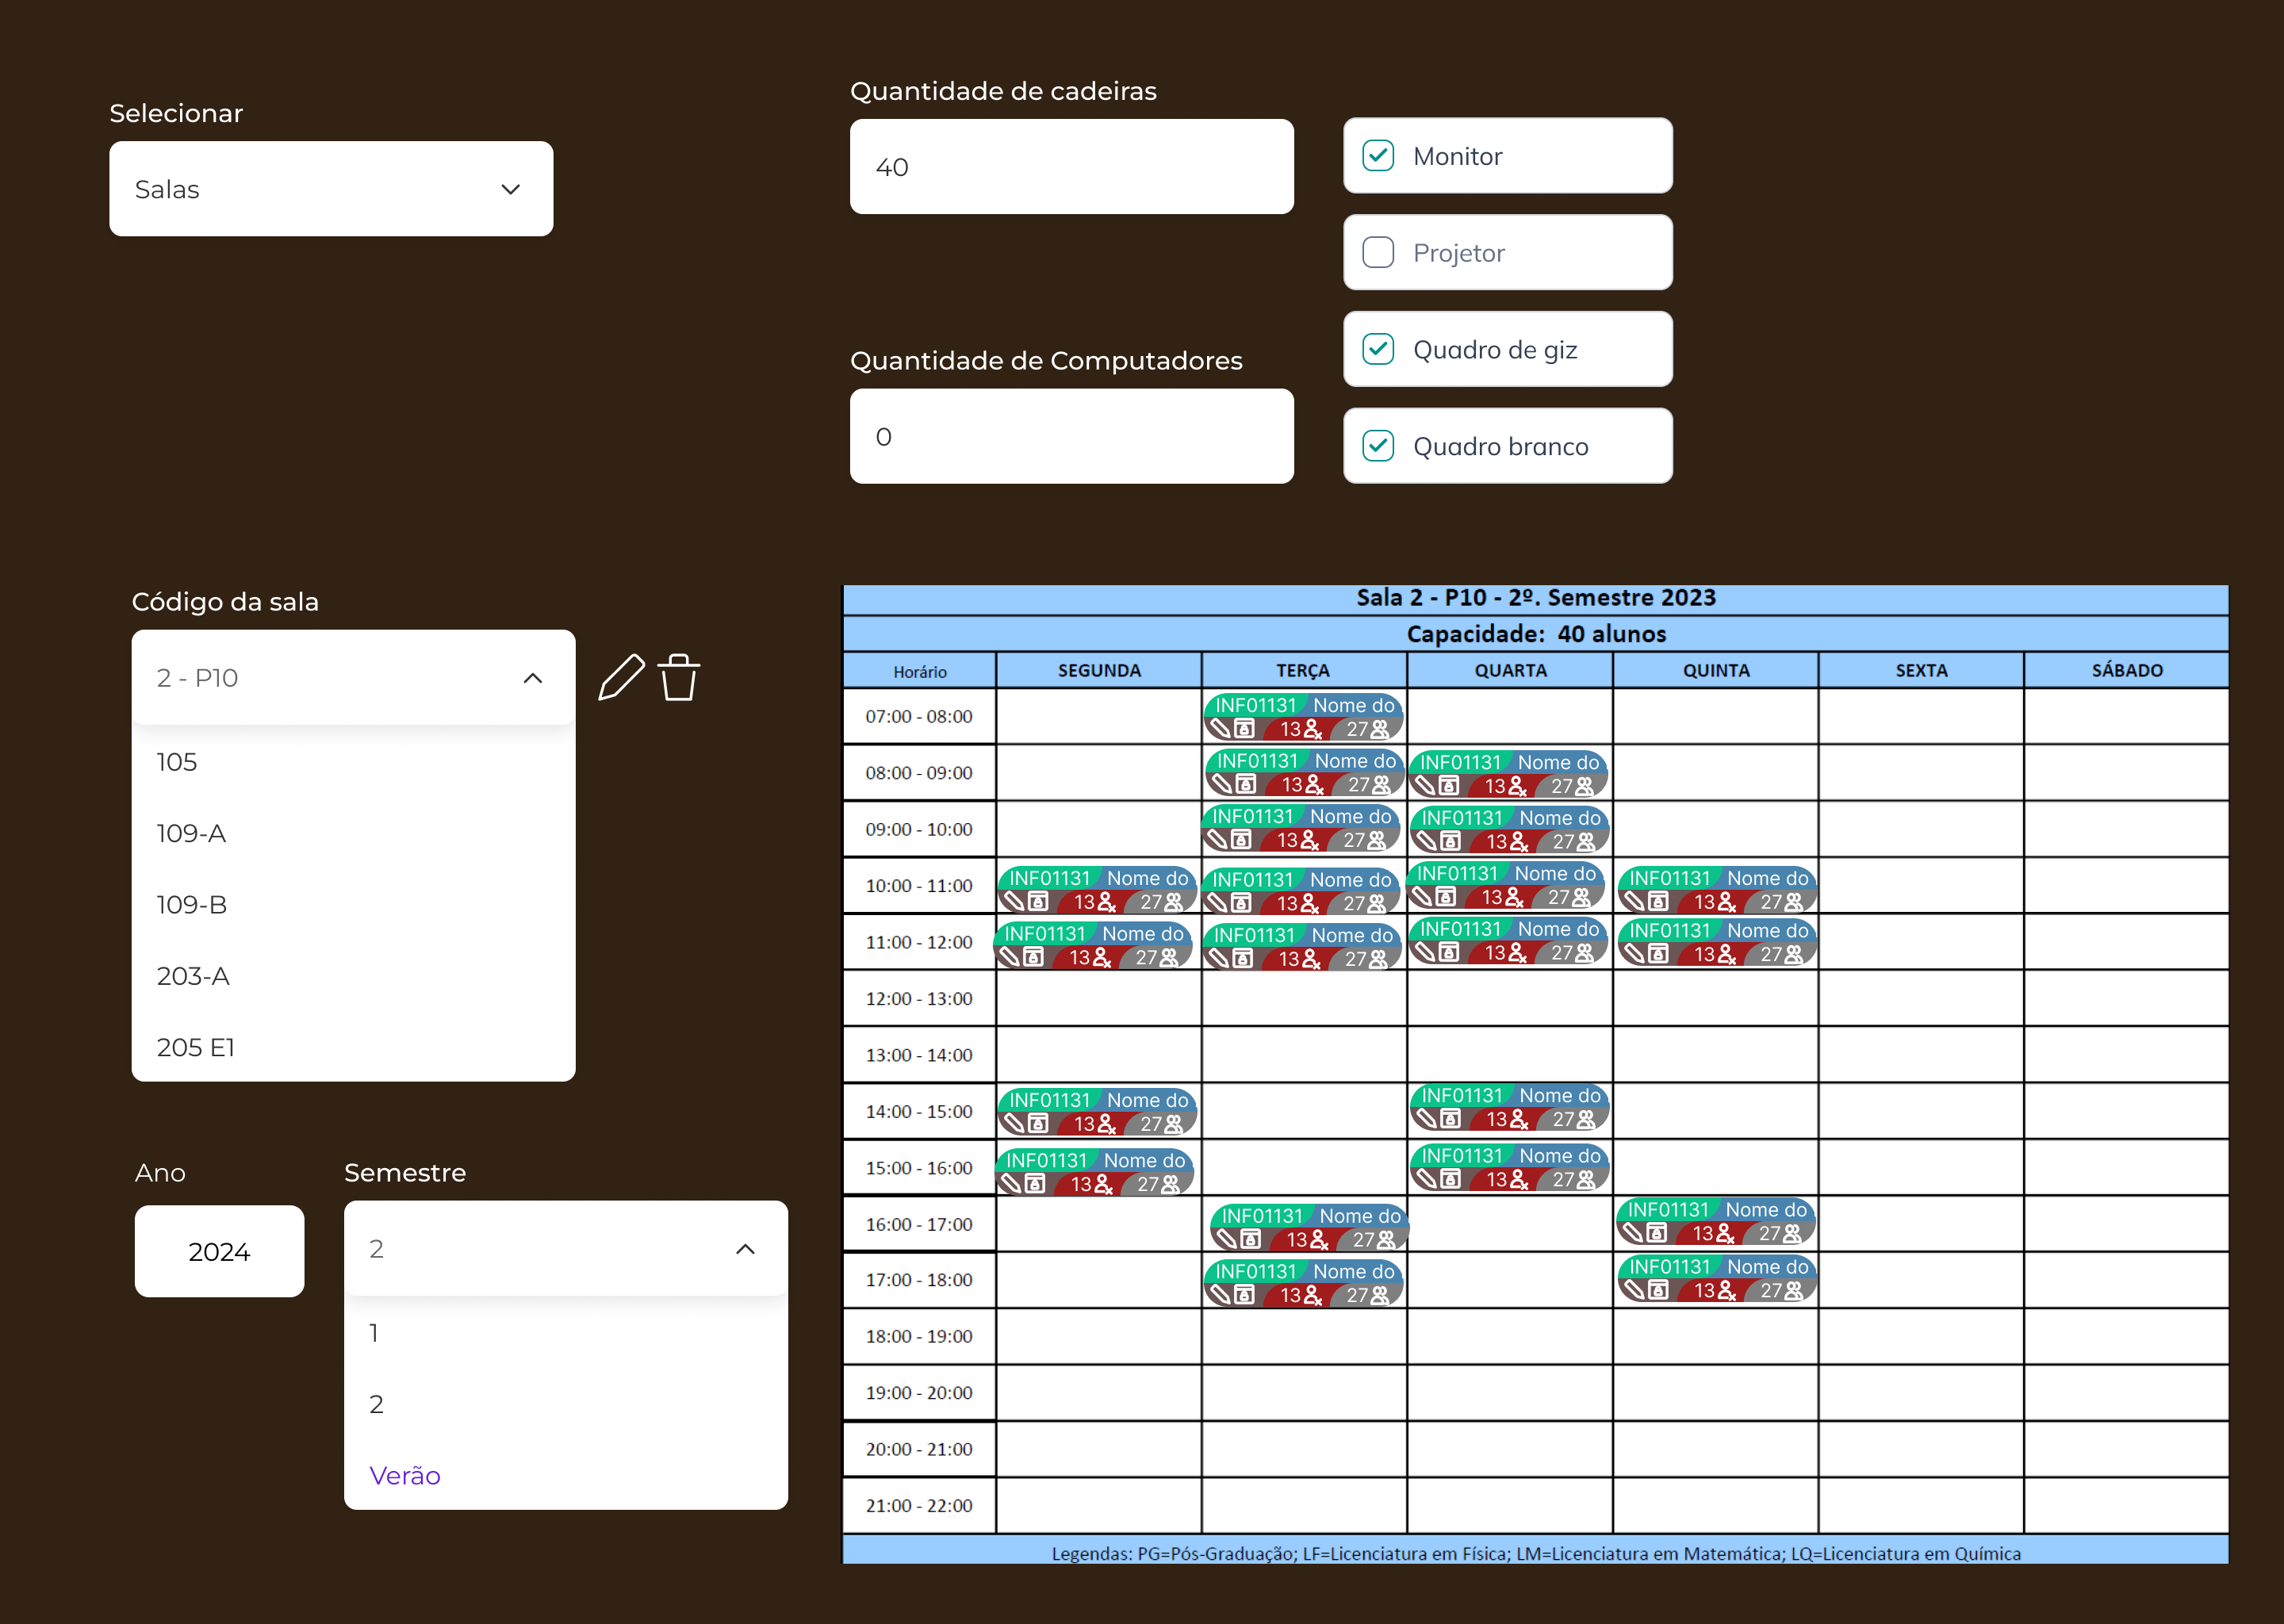
\includegraphics[scale=0.8]{files/img/Experimentos/SituacaoInicial.png}
% \legend{\selfAuthor}
% \end{figure}    % Distribuição inicial das disciplinas
% ![Alt text](img/Experimentos/SituacaoInicial.png)

% Nessa imagem, vemos que algumas das turmas foram alocadas em salas que não possuem a capacidade necessária para a quantidade de alunos que demandam a disciplina. Além disso, vemos que algumas das turmas foram alocadas em horários que não condizem com a preferência dos professores.

% \begin{figure}[htbp]\centering
% \caption{\label{DistribuicaoAprimorada}Disposição aprimorada das disciplinas}
% 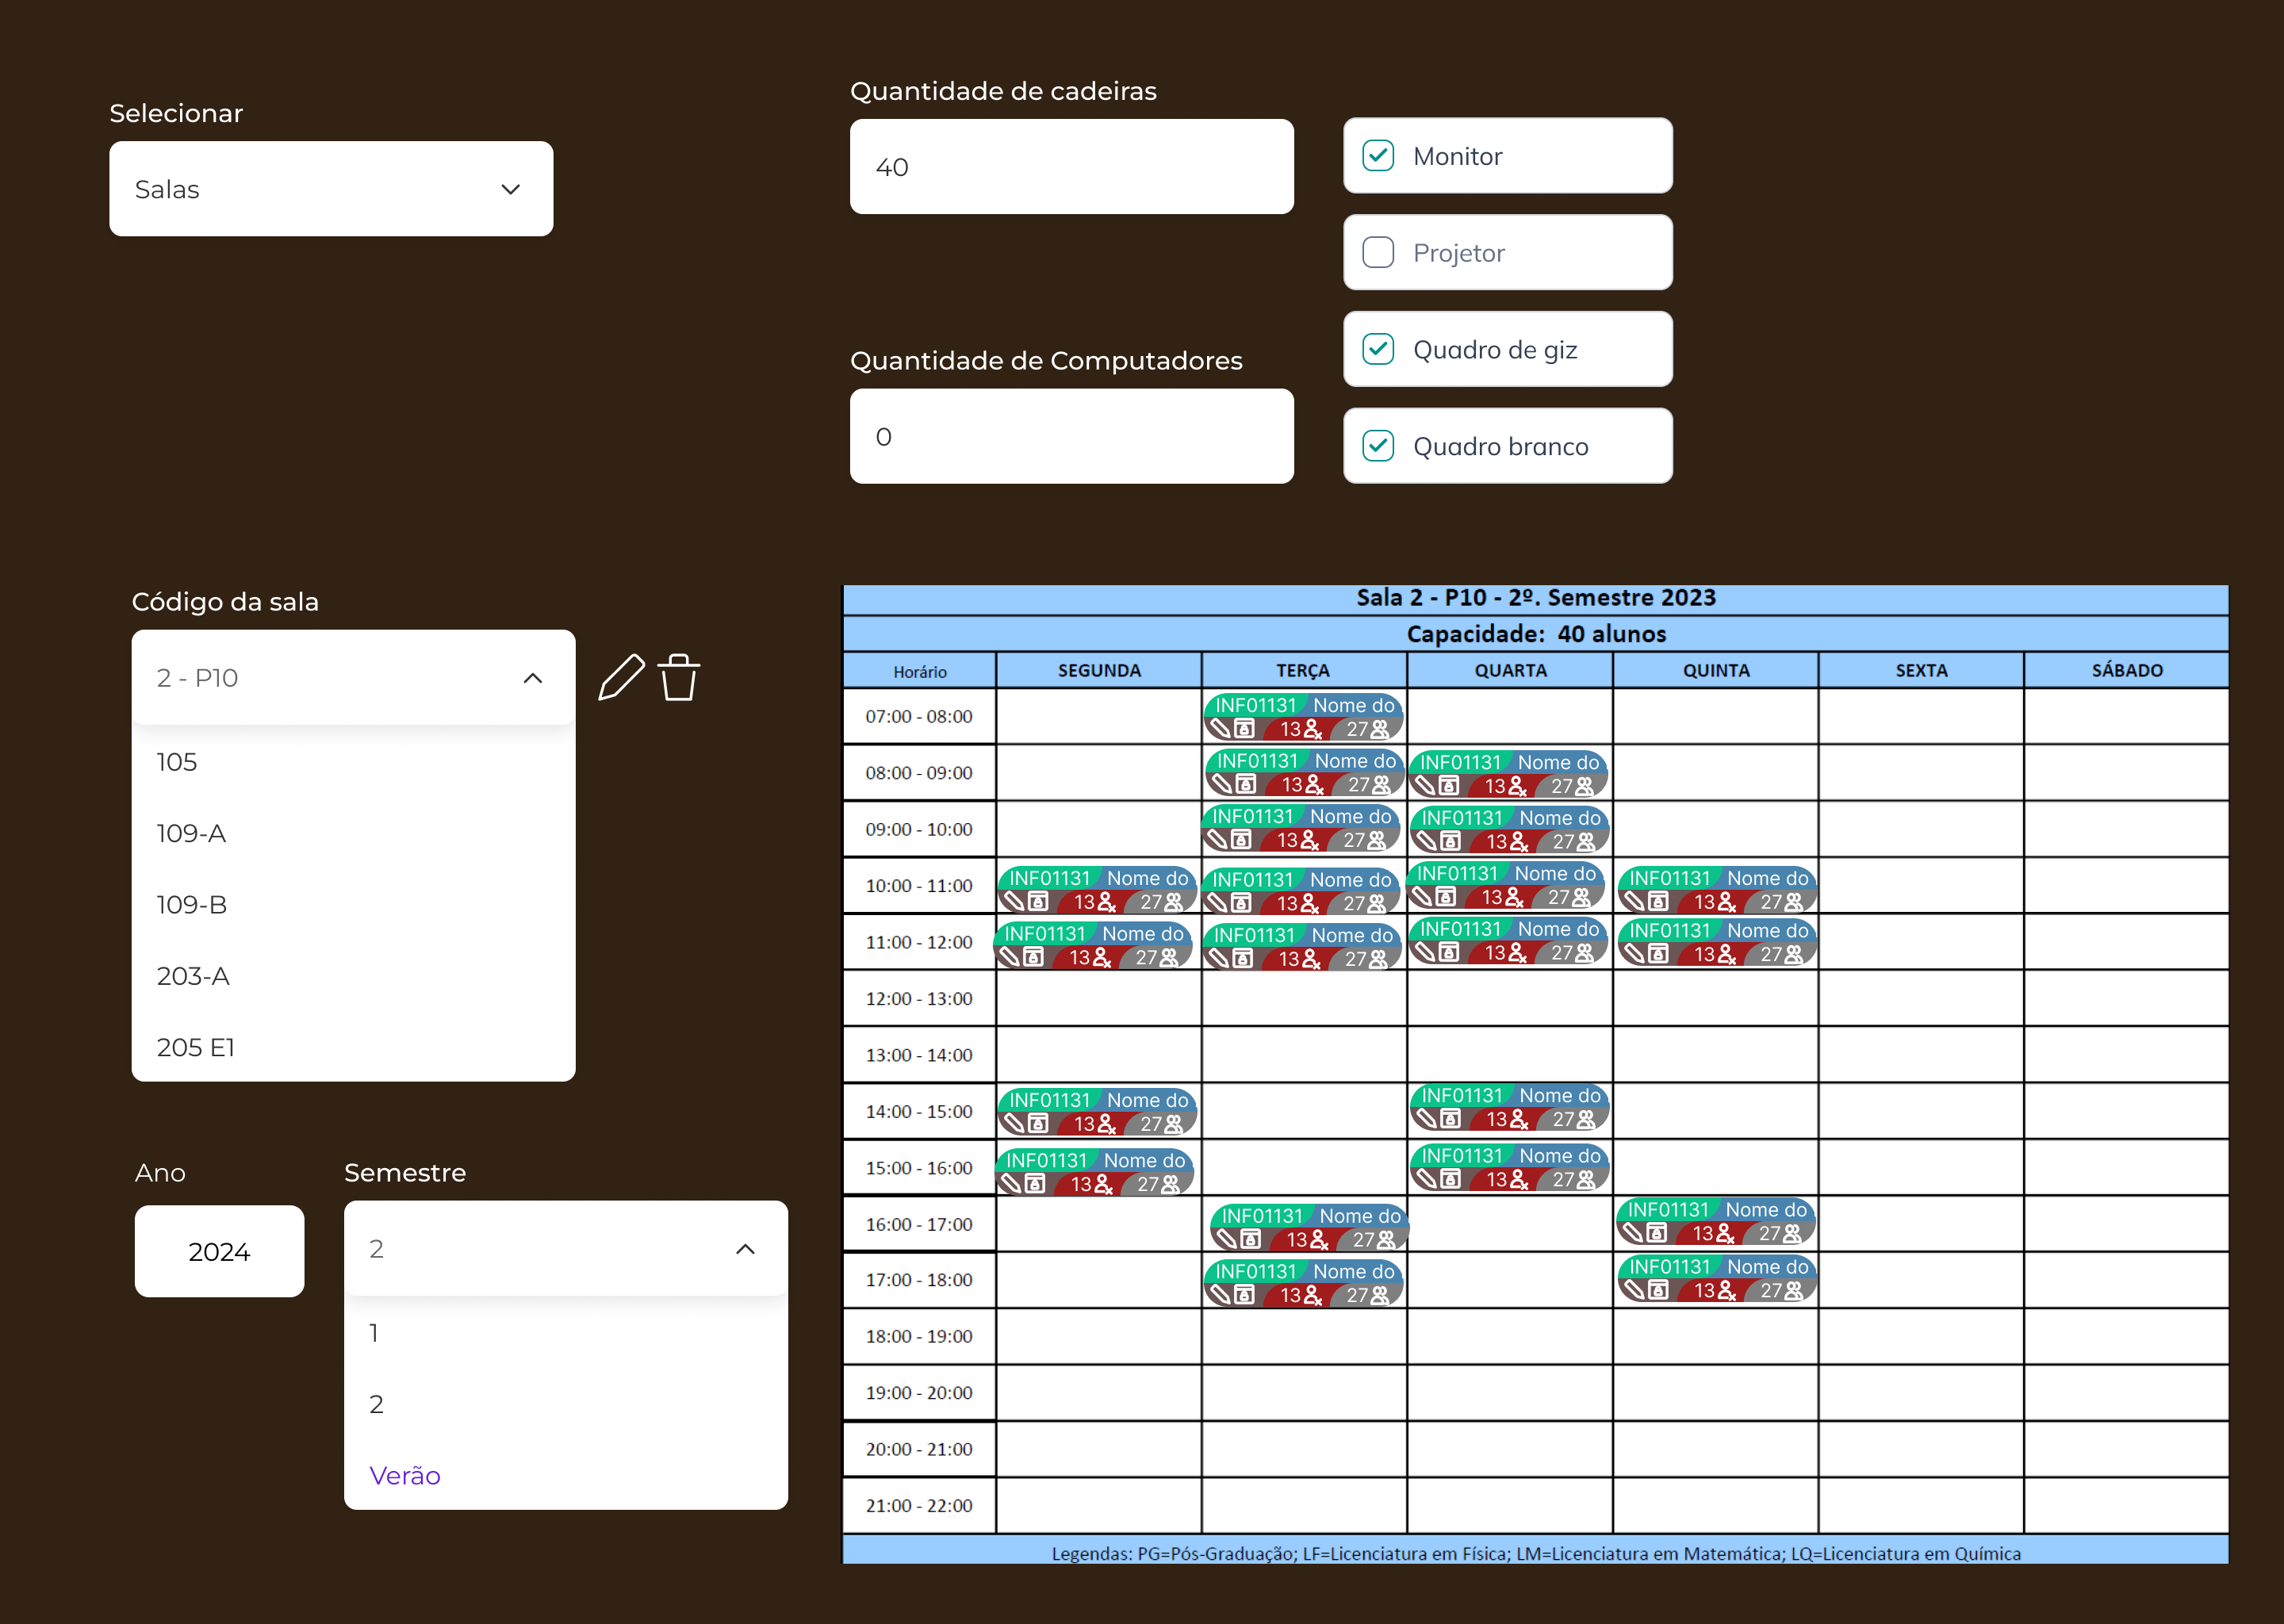
\includegraphics[scale=0.8]{files/img/Experimentos/Aprimoramento.png}
% \legend{\selfAuthor}
% \end{figure}    % Distribuição aprimorada das disciplinas
% ![Alt text](img/Experimentos/Aprimoramento.png)

Com as alterações na tabela inicial de distribuição de disciplinas, foi possível obter uma grade horária com menos conflitos e que se aproxima mais da preferência dos professores.


% \chapter{Resultados} \label{chap:resultados} % ### 7.

% O QUE DEVERIA TER INTERVALO É ENTRE O FIM DAS INSCRIÇÕES E O INÍCIO DAS AULAS

% adicionar também a possibilidade da mudança informal do horário

\section{Sistema} % ### 7.1.

O sistema desenvolvido atualmente pode ser acessado através \href{https://jvfd3.github.io/timetabling-UENF/}{deste link} \url{https://jvfd3.github.io/timetabling-UENF/}.

\section{Solução Ótima} % ### 7.2.

\section{Alternativas Burocráticas} % ### 7.2.

Além da busca pela solução ótima, o presente trabalho também se propõe a buscar métodos ainda mais alternativos para se amenizar a problemática abordada. Sendo, de forma simples, o uso de meios burocráticos disponíveis na instituição que abre alguns caminhos para uma maior praticidade no processo de resolução do problema. Entretanto, é necessário que se tenha em mente que a burocracia é um processo lento e que pode ser desgastante, sendo até mesmo esperado que não seja desejado por parte dos construtores da grade horária.

Essas alternativas não geram por si só uma solução para o problema, em termos metafóricos, se o sistema é a engrenagem que faz a máquina funcionar, as alternativas burocráticas são o óleo que pode fazer a engrenagem funcionar de forma mais suave, mesmo que não seja estritamente necessário.

\subsection{Tempo de elaboração das grades} % #### 7.1.1.

Durante as entrevistas do \autoref{chap:instituicao} da \autoref{sec:entrevistas}, uma alternativa válida para a amenização da problemática abordada é a alteração do calendário anual da UENF que define férias de duas semanas entre os semestres. Caso seu calendário seja alterado para que as férias sejam de três semanas, o problema de agendamento teria maior tempo para ser resolvido, assim fazendo com que a solução ótima seja provável de ser alcançada.

Mais especificamente: no atual semestre (2024.1), o encerramento do semestre está previsto para o dia 6 de julho. Já o prazo limite para o cadastro de novas

% Abreviados
\begin{table}[H] \centering \caption{Calendário Acadêmico da SECACAD de 2023.1 (simplificado para mostrar apenas os eventos relevantes)} \label{tab:calendario_SECACAD-2023.1}
  \begin{tabular}{| l r |}
    \hline
    \textbf{Atividades}                                              & \textbf{Data} \\
    \hline
    Prazo limite de cad. de nov. discip. a serem ofer. em 2023.1     & até 20/01     \\
    Prazo limite para criação de turmas a serem oferecidas em 2023.1 & 20/01 a 15/02 \\
    Renovação de matrícula de 2023.1                                 & 28/02 a 03/03 \\
    Início do período letivo de 2023.1                               & 06/03         \\
    Inclusão e exclusão de disciplinas                               & 06/03 à 20/03 \\
    Encerramento do período letivo de 2023.1                         & 07/07         \\
    Prazo limite: Entrega dos resultados à SECACAD                   & 14/07         \\
    \hline
  \end{tabular}
\end{table}

% Citar o Estatuto da forma correta.

Segundo o Artigo 28 do Estatuto da UENF, compete à secretaria acadêmica a elaboração da proposta de calendário escolar para que seja aprovado pelo Colegiado Acadêmico. Enquanto que o Artigo 63 da seção 2 do capítulo 1, informa que os calendários do curso de graduação devem ser aprovados pelas correspondentes câmaras, com observância do calendário da universidade.
\begin{comment}
\begin{table}[H] \centering
  \caption{Calendário Acadêmico da SECACAD de 2023.1 (simplificado para mostrar apenas os eventos relevantes)}
  \label{tab:calendario_SECACAD-2023.1}
  \begin{tabular}{| l r |}
    \hline
    \textbf{Atividades}                                                                           & \textbf{Data}           \\
    \hline
    Prazo limite de cadastro de novas disciplinas a serem oferecidas no 1º período letivo de 2023 & até 20/01/2023          \\
    Prazo limite para criação de turmas a serem oferecidas no 1º período letivo de 2023           & 20/01/2023 a 15/02/2023 \\
    Renovação de matrícula do 1º período letivo/2023                                              & 28/02 a 03/03           \\
    Início do 1º período letivo de 2023                                                           & 06/03                   \\
    Inclusão e exclusão de disciplinas                                                            & 06/03 à 20/03           \\
    Encerramento do 1º período letivo de 2023                                                     & 07/07                   \\
    \hline
  \end{tabular}
\end{table}

Logo, quanto à alteração do calendário acadêmico, a alteração mostra-se como possível, sendo necessário apenas que o processo burocrático necessário seja enfrentado.
\begin{table}[H] \centering
  \caption{Calendário Acadêmico da SECACAD de 2023.2 (simplificado para mostrar apenas os eventos relevantes)}
  \label{tab:calendario_SECACAD-2023.2}
  \begin{tabular}{| l r |}
    \hline
    \textbf{Atividades}                                                                           & \textbf{Data} \\
    \hline
    Prazo limite de cadastro de novas disciplinas a serem oferecidas no 2º período letivo de 2023 & até 14/07     \\
    Prazo limite: Entrega dos resultados à SECACAD                                                & 14/07         \\
    Prazo limite para criação de turmas a serem oferecidas no 2º período letivo de 2023           & 17 a 28/07    \\
    Renovação de matrícula do 2º período letivo/2023                                              & 01/08 a 04/08 \\
    Início do 2º período letivo de 2023                                                           & 07/08         \\
    Inclusão e exclusão de disciplinas                                                            & 14 a 21/08    \\
    Encerramento do 2º período letivo de 2023                                                     & 08/12         \\
    Prazo limite: Entrega dos resultados à SECACAD                                                & 15/12         \\
    \hline
  \end{tabular}
\end{table}
\end{comment}

\subsection{Alteração forçada de horários} % #### 7.1.2.
\begin{table}[H] \centering \caption{Calendário Acadêmico da SECACAD de 2023.2 (simplificado para mostrar apenas os eventos relevantes)} \label{tab:calendario_SECACAD-2023.2}
  \begin{tabular}{| l r |}
    \hline
    \textbf{Atividades}                                              & \textbf{Data} \\
    \hline
    Prazo limite de cad. de nov. discip. a serem ofer. em 2023.2     & até 14/07     \\
    Prazo limite para criação de turmas a serem oferecidas em 2023.2 & 17 a 28/07    \\
    Renovação de matrícula de 2023.2                                 & 01/08 a 04/08 \\
    Início do período letivo de 2023.2                               & 07/08         \\
    Inclusão e exclusão de disciplinas                               & 14 a 21/08    \\
    Encerramento do período letivo de 2023.2                         & 08/12         \\
    Prazo limite: Entrega dos resultados à SECACAD                   & 15/12         \\
    \hline
  \end{tabular}
\end{table}

Segundo o parágrafo primeiro do artigo 36 das Normas de Graduação, ``qualquer alteração de horário/turno após o período de matrícula deverá ter a anuência por escrito de todos os discentes matriculados na turma''. Seguindo ao segundo parágrafo do mesmo artigo, temos que ``a alteração de horário das aulas da turma deverá ter a anuência da Coordenação de Curso e a ciência do Chefe do Laboratório responsável pela disciplina''.

Outra alternativa que aproveita de uma brecha nas normas supracitadas é a possibilidade de se criar novas turmas para as disciplinas que possuem horários conflitantes, assim direcionando os alunos para que se desinscrevam da turma anterior.
\begin{table}[H] \centering \caption{Calendário Acadêmico de 2023 (simplificado para mostrar apenas os eventos relevantes)} \label{tab:calendario_2023-Enxuto}
  \begin{tabular}{| c r l c |}
    \hline
    \textbf{Vigência} & \textbf{Fase}         & \textbf{Atividades}                              & \textbf{Data} \\
    \hline
    %2022.2 &\textbf{Fim}          & período letivo                                           & 14/12/22      \\
    %2022.2 &\textbf{\textit{Fim}} & entrega dos resultados à SECACAD                         & 21/12/22      \\
    2023.1            & \textbf{\textit{Fim}} & cadastro de novas disciplinas a serem oferecidas & 20/01/23      \\
    2023.1            & \textbf{Início}       & criação de turmas a serem oferecidas             & 20/01/23      \\
    2023.1            & \textbf{Fim}          & criação de turmas a serem oferecidas             & 15/02/23      \\
    2023.1            & \textbf{Início}       & renovação de matrícula                           & 28/02/23      \\
    2023.1            & \textbf{Fim}          & renovação de matrícula                           & 03/03/23      \\
    2023.1            & \textbf{Início}       & período letivo                                   & 06/03/23      \\
    2023.1            & \textbf{Início}       & inclusão e exclusão de disciplinas               & 06/03/23      \\
    2023.1            & \textbf{Fim}          & inclusão e exclusão de disciplinas               & 20/03/23      \\
    2023.1            & \textbf{Fim}          & período letivo                                   & 07/07/23      \\
    2023.1            & \textbf{\textit{Fim}} & entrega dos resultados à SECACAD                 & 14/07/23      \\
    2023.2            & \textbf{\textit{Fim}} & cadastro de novas disciplinas a serem oferecidas & 14/07/23      \\
    2023.2            & \textbf{Início}       & criação de turmas a serem oferecidas             & 17/07/23      \\
    2023.2            & \textbf{Fim}          & criação de turmas a serem oferecidas             & 28/07/23      \\
    2023.2            & \textbf{Início}       & renovação de matrícula                           & 01/08/23      \\
    2023.2            & \textbf{Fim}          & renovação de matrícula                           & 04/08/23      \\
    2023.2            & \textbf{Início}       & período letivo                                   & 07/08/23      \\
    2023.2            & \textbf{Início}       & inclusão e exclusão de disciplinas               & 14/08/23      \\
    2023.2            & \textbf{Fim}          & inclusão e exclusão de disciplinas               & 21/08/23      \\
    2023.2            & \textbf{Fim}          & período letivo                                   & 08/12/23      \\
    2023.2            & \textbf{\textit{Fim}} & entrega dos resultados à SECACAD                 & 15/12/23      \\
    %2024.1 &\textbf{Início}       & renovação de matrícula                                   & 26/02/24      \\
    %2024.1 &\textbf{Fim}          & renovação de matrícula                                   & 01/03/24      \\
    %2024.1 &\textbf{Início}       & período letivo                                           & 04/03/24      \\
    \hline
  \end{tabular}
\end{table}

Sendo assim possível alterar os horários de aula caso seja necessária para que haja uma melhora geral na distribuição das turmas na grade horária, mais uma vez sendo necessário superar o processo burocrático necessário.

% \chapter{Conclusões} % ## 8. Conclusões

% CONCLUIR CAPÍTULO POR CAPÍTULO

O problema de organização de grade horária no ensino superior tem sido amplamente estudado por diversos pesquisadores. Devido sua natureza multidimensional e com forte tendência a especificidades, este campo de estudo se mostra como amplo e complexo.

Através da revisão bibliográfica, foi possível observar que a maioria dos trabalhos se foca em um método heurístico de solução, onde se busca uma solução ótima, ou próxima do ótimo, através de um método de busca. Entretanto, o presente trabalho se propõe a uma abordagem diferente, onde se busca uma solução boa o suficiente para que seja utilizada na prática, mesmo que não seja ótima, isso através do método de manipulação manual dos dados.

Para este fim foi desenvolvido um sistema de suporte à decisão para auxiliar os setores da Universidade Estadual do Norte Fluminense Darcy Ribeiro (UENF) responsáveis pela criação de grades horárias. O sistema foi desenvolvido com o intuito de ser utilizado como uma ferramenta auxiliar, onde os usuários possam manipular os dados de forma mais intuitiva e visual, assim reduzindo a necessidade de retrabalho e aumentando a produtividade.

O sistema permite que as quatro operações básicas de armazenamento persistente, sendo elas a criação, leitura, edição e deleção de dados. Com isso, os usuários podem adicionar manualmente as informações referentes ao trabalho de criação de grade horária de forma centralizada, assim reduzindo a necessidade de se lidar com diversos arquivos e planilhas. Facilitando também a visualização de informações, como a alocação de turmas, que pode ser visualizada de forma gráfica, assim facilitando a identificação de conflitos e problemas. O que consequentemente tende a agilizar o processo de busca por novas soluções e a redução dos conflitos.

% <!-- Tendo atingido este objetivo, espera-se que o sistema possa ser utilizado na prática, e que possa ser aprimorado e melhorado com o tempo. -->

\section{Trabalhos futuros} % ## 8.1 Trabalhos futuros

Como trabalhos futuros, vê-se uma ampla gama de pesquisa e aprimoramento ao presente trabalho, visto que este busca um método alternativo de solução ao mesmo problema abordado por outros dois pesquisadores em tempos anteriores. Pode-se então elaborar uma conexão entre o atual sistema e modelos aos métodos heurísticos propostos, permitindo então uma abordagem híbrida humano-computador na busca da grade horária ótima. Sugere-se inclusive o estudo sobre a aplicação de métodos de programação inteira, visto que através da revisão bibliográfica este método apresentou consideráveis resultados.

Assim como os modelos anteriores apresentaram diversas incongruências com a realidade prática da universidade estudada, é esperado que este trabalho acabe por trilhar o mesmo caminho, visto que o problema em questão realmente apresenta grande parte de sua complexidade no entendimento e modelagem de como as diversas partes da instituição interagem entre si, porém, espera-se que este documento possa servir como uma boa base para o entendimento de sua estrutura.

Quanto ao software, mesmo que o prioritário seja a sua funcionalidade, é esperado que o seu design seja o mais intuitivo, fluido e prático quanto for possível. Sendo esta tarefa direcionada mais à experiência do usuário, possivelmente tangenciando o problema central de construção de grades horárias.

Considerando que as duas tentativas anteriores resultaram em métodos que embora atingissem seu objetivo, não foram implementados na prática, tem-se como esperado que o mesmo ocorra com este trabalho. Com isso, espera-se que em trabalhos futuros se estude e analise os motivos de falha do uso prático do atual sistema.

\subsection*{Apelo}

Eu gostaria de deixar aqui um alerta para quem for utilizar este documento como base para futuros trabalhos: a maior dificuldade a ser superada é o fator organizacional. A minha percepção é de que a UENF atualmente se encontra tal qual um osso quebrado que se regenerou sem o uso de gesso para o fixar no local certo: funciona, mas não tão bem quanto seria capaz. E, assim como no caso ósseo, para que você atinja um resultado ótimo, certamente terá que quebrar algumas estruturas já consolidadas para que possa reorganizá-las de forma mais eficiente.

Neste trabalho tentei pavimentar o caminho na direção que acredito ser a mais apropriada para a adoção do sistema. Nesse caminho, acabei abrindo mão de meus desejos pessoais que envolviam o sistema direcionado às demandas dos alunos, visto que, mesmo que atingisse um resultado ótimo aos alunos, nada adiantaria se o sistema não fosse adequado àqueles que o usarão. Eu espero que este trabalho não se torne apenas mais uma monografia que será esquecida em uma prateleira, mas sim que ele possa ser utilizado como um guia para a construção do sistema que um dia sonhei em desenvolver.

Se você chegou até aqui, eu agradeço por ter lido este trabalho. E, se você for um estudante da UENF, eu peço que você não desista de lutar por um ensino melhor. A UENF é uma instituição que tem um grande potencial, e eu acredito que ela pode ser muito mais do que é hoje. Eu espero que este trabalho possa ser um pequeno passo na direção de um futuro melhor para a nossa universidade.

Caso o sistema ainda esteja em funcionamento, excelente, isso significa que consegui atingir um de meus objetivos, então, continue a aprimorá-lo. Caso contrário, torne como seu objetivo consertar os meus erros. Descubra o motivo da não adoção do sistema e corrija-o. E, se possível, me avise, eu adoraria saber que o meu trabalho não foi em vão.

Além do desenvolvimento da monografia como objetivo para a conclusão do curso, o que desejo é conseguir auxiliar as pessoas em suas atividades diárias. Ainda mais se considerarmos que este sistema, se bem executado, tende a ajudar semestralmente centenas, senão milhares, de alunos e professores semestralmente.


\postextual{} % --- INÍCIO DOS ELEMENTOS PÓS-TEXTUAIS ---

\bibliography{files/referencias}
 % --- Referências bibliográficas ---
% \begin{apendicesenv} % Imprime uma página indicando o início dos apêndices
  \chapter{Formulário de pesquisa quantitativa}

  Pesquisa quantitativa de alunos da UENF sobre distribuição e oferta de disciplinas

  \section*{Seção 1: Pesquisa quantitativa de alunos da UENF sobre distribuição e oferta de disciplinas}

  Olá! Desde já agradeço por ceder em torno de 4 minutos do seu tempo para responder a este formulário usando o seu e-mail institucional. Considerando que nosso tempo é valioso, vamos direto ao objetivo:

  Me chamo João Vítor Fernandes Dias, estudante de Ciência da Computação na UENF, e estou fazendo minha Monografia. Ela trata da elaboração de um sistema para a coordenação de curso poder analisar mais facilmente quais são as disciplinas que serão disponibilizadas a cada semestre e a quais salas e professores serão atribuídas.

  O objetivo da minha monografia é conseguir tornar mais eficiente a distribuição das disciplinas, para que se resulte em um conjunto de disciplinas ofertadas com melhor qualidade. Espera-se com isso que as demandas de disciplina dos alunos sejam melhor atendidas, assim como as preferências de horários dos professores.

  Este formulário tem como objetivo avaliar a sua satisfação em relação ao processo de inscrição semestral nas disciplinas.

  \section*{Seção 2: Sobre você}

  Nesta seção, peço que informe algumas características suas para que a análise estatística se torne mais rica.

  \begin{itemize}
    \item \textbf{Pergunta:} Qual o seu nome?
    \item \textbf{Opções de resposta}
          \begin{enumerate}
            \item Administração Pública
            \item Agronomia
            \item Biologia (Licenciatura)
            \item Ciência da Computação
            \item Ciências Biológicas (bacharelado)
            \item Ciências Sociais
            \item Engenharia Civil
            \item Engenharia de Exploração e Produção de Petróleo
            \item Engenharia de Produção
            \item Engenharia Metalúrgica
            \item Engenharia Meteorológica
            \item Física (licenciatura)
            \item Matemática (Licenciatura)
            \item Medicina Veterinária
            \item Pedagogia (Licenciatura)
            \item Química (Licenciatura)
            \item Zootecnia
            \item Outro
          \end{enumerate}
  \end{itemize}

  \begin{itemize}
    \item \textbf{Pergunta:} Em que ano você ingressou na UENF?
    \item \textbf{Opções de resposta}
          \begin{enumerate}
            \item 2023
            \item 2022
            \item 2021
            \item 2020
            \item 2019
            \item 2018
            \item 2017
            \item 2016
            \item 2015
            \item 2014
            \item 2013
            \item Outro
          \end{enumerate}
  \end{itemize}

  \section*{Seção 3: Pesquisa de satisfação}

  Agora serão feitas algumas perguntas em relação à sua satisfação com algumas características da Universidade.

  Abaixo, estão algumas perguntas gerais em relação à sua satisfação com a distribuição de disciplinas semestralmente.

  \begin{itemize}
    \item \textbf{Perguntas}
          \begin{enumerate}
            \item Salas: Você já teve que mudar de sala por falta de algum acessório como quadro, projetor ou monitor?
            \item Salas: Você já teve aula cuja sala não dispunha de carteiras o suficiente?
            \item Vagas: Você já quis entrar em uma disciplina, mas ela não tinha vaga?
            \item Vagas: Você já ficou acordado após meia-noite por medo de não ter vaga para as disciplinas que deseja cursar?
            \item Conflitos: Você já deixou de se inscrever em uma disciplina por causa de conflito de horário?
            \item Preferências: Você já preferiu não se inscrever em uma disciplina para cursá-la em outro momento mais oportuno?
            \item Opiniões: Você acha que a universidade deveria oferecer horários diferentes para as disciplinas mais demandadas para evitar conflitos com outras disciplinas?
          \end{enumerate}
    \item \textbf{Opções de resposta}
          \begin{enumerate}
            \item Sim
            \item Não
            \item Outro
          \end{enumerate}
  \end{itemize}

  \section*{Seção 4: Preferências pessoais}

  Esta seção visa saber um pouco mais sobre as suas preferências pessoais quanto a escolha das disciplinas ofertadas.

  \begin{itemize}
    \item \textbf{Pergunta:} Você prefere disciplinas distribuídas ao longo da semana ou acumuladas em poucos dias?
    \item \textbf{Opções de resposta}
          \begin{enumerate}
            \item Distribuídas ao longo da semana
            \item $\sim$
            \item Não tenho preferência
            \item $\sim$
            \item Acumuladas em poucos dias
          \end{enumerate}
  \end{itemize}

  \begin{itemize}
    \item \textbf{Pergunta:} Você prefere disciplinas na parte da manhã ou na parte da tarde?
    \item \textbf{Opções de resposta}
          \begin{enumerate}
            \item na parte da manhã
            \item $\sim$
            \item Não tenho preferência
            \item $\sim$
            \item na parte da tarde
          \end{enumerate}
  \end{itemize}

  \begin{itemize}
    \item Como você lida com conflitos de horário entre as disciplinas que deseja cursar?
    \item \textbf{Opções de resposta} (Permite múltiplas escolhas)
          \begin{itemize}
            \item Escolho a mais difícil
            \item Escolho a mais fácil
            \item Escolho a que tem mais créditos
            \item Escolho a que prefiro
            \item Escolho a que ``prende'' mais matérias
            \item Escolho a disciplina mais concorrida
            \item Outro...
          \end{itemize}
  \end{itemize}

  \section*{Seção 5: Experiências passadas com atrasos e disciplinas}

  Aqui estão algumas perguntas relacionadas à divergência entre o período esperado de conclusão das disciplinas VS o período em que elas de fato são realizadas.

  \begin{itemize}
    \item \textbf{Pergunta:} Quanto tempo (em períodos) você já teve que esperar para fazer uma disciplina da sua grade?
    \item Descrição: Exemplo hipotético: estou no 6º período e estou desde o 4º período tentando me inscrever em uma disciplina, mas ela não foi oferecida ou não teve vaga, então tive que esperar 2 períodos.
    \item \textbf{Opções de resposta}: 0, 1, 2, 3, 4, 5, 6, 7, 8, 9, 10
  \end{itemize}

  \begin{itemize}
    \item \textbf{Pergunta:} Qual foi a quantidade máxima de períodos que você se distanciou de uma disciplina de determinado período?
    \item Descrição: Exemplo hipotético: estou no 6º período da faculdade, mas ainda estou cursando uma disciplina do 3º período, pois escolhi não fazer antes, ou ainda não obtive a aprovação, logo, me distanciei 3 períodos do esperado.
    \item \textbf{Opções de resposta}: 0, 1, 2, 3, 4, 5, 6, 7, 8, 9, 10
  \end{itemize}

  \section*{Seção 6: Você acha que a distribuição de disciplinas semestrais é...}

  \begin{itemize}
    \item Classificações
          \begin{itemize}
            \item Justa (feita de acordo a atender os desejos da maioria)
            \item Variada (bem diversa e abrange diversos interesses)
            \item Contínua (oferecida de forma a ter aulas sequenciais)
            \item Eficiente (bem sucedida em atender aos desejos dos alunos)
            \item Distribuída (bem espaçada ao longo da semana)
            \item Satisfatória (agradável aos meus desejos pessoais)
          \end{itemize}
    \item \textbf{Descrição:} Exemplo hipotético: estou no 6º período da faculdade, mas ainda estou cursando uma disciplina do 3º período, pois escolhi não fazer antes, ou ainda não obtive a aprovação, logo, me distanciei 3 períodos do esperado.
          \begin{enumerate}
            \item Discordo completamente
            \item $\sim$
            \item $\sim$
            \item $\sim$
            \item Concordo completamente
          \end{enumerate}
  \end{itemize}


  \section*{Seção 7: Opcional}

  Por fim, deixo aqui um espaço caso deseje compartilhar algum comentário, opinião ou sugestão quanto ao meu trabalho ou formulário.

  Escreva aqui caso haja algo que gostaria de comentar, opinar ou sugerir. Tudo bem deixar em branco, suas informações já foram de grande ajuda.

  \begin{itemize}
    \item Campo de texto livre
  \end{itemize}

\end{apendicesenv}

% ----------------------------------------------------------
% Anexos
% ----------------------------------------------------------

% ---
% Inicia os anexos
% ---
% \begin{anexosenv}

% % Imprime uma página indicando o início dos anexos
% \partanexos

% % ---
% %\chapter{Morbi ultrices rutrum lorem.}
% % ---
% \lipsum[30]

% % ---
% %\chapter{Cras non urna sed feugiat cum sociis natoque penatibus et magnis dis
% %parturient montes nascetur ridiculus mus}
% % ---

% \lipsum[31]

% % ---
% %\chapter{Fusce facilisis lacinia dui}
% % ---

% \lipsum[32]

% \end{anexosenv}


\end{document}
